\section{Bi-continuous and non-particulate structures}

\subsection{Stochastic models of disordered porous materials}~\\

The stochastic models implemented base mainly on the paper from \cite{Gommes2018}, where the different existing models have been  compared. The "dead leaves"- model as well as the boolean models described here assume for simplicity spheres for the grains where the covariogram of a sphere is given by
\begin{align}\label{eq:covariogram_sphere}
K(r,R) &= \frac{4\pi}{3}R^3\left(1-\frac{r}{2R}\right)^2\left(1+\frac{r}{4R}\right)\Theta(2R-r)
\end{align}
where $\Theta()$ is Heavyside's step function, taking the value 1 for a positive argument and 0 otherwise. A LogNormal size distribution $p_\mathrm{LN}(R)$ can be taken into account analytically
\begin{align}
  K_\mathrm{LN}(r) =& \int_0^\infty  p_\mathrm{LN}(R) K(r,R) \mathrm{d}R \nonumber\\
       \begin{split}
            =& \frac{\pi}{24} r^3 \left(1+\mathrm{Erf}\left(\frac{\ln(2\mu/r)}{\sqrt{2}\sigma}\right)\right) -\\
            & \frac{\pi}{2}\mu^2r e^{2\sigma^2} \left(1+\mathrm{Erf}\left(\frac{2\sigma^2+\ln(2\mu/r)}{\sqrt{2}\sigma}\right)\right) +\\
            & \frac23 \pi e^{9\sigma^2/2}\mu^3\left(1+\mathrm{Erf}\left(\frac{3\sigma^2+\ln(2\mu/r)}{\sqrt{2}\sigma}\right)\right)
       \end{split} \label{eq:covariogram_sphere_LogNorm}
\end{align}
with
\begin{align}
  p_\mathrm{LN}(R,\mu,\sigma) &=  \frac{1}{R\sigma \sqrt{2 \pi}}\exp\left(-\frac{1}{2}\left(\frac{\ln R -
        \ln\mu}{\sigma}\right)^2\right)
\end{align}
The Debye correlation function $\gamma(r)$ needs to be expressed in terms of the covariagram function $K(r)$ and the volume fractionas $\phi_0=1-\phi_1$ of the pores or solid material. The knowledge of $\gamma(r)$ then allows to calculate the scattering intensity via
\begin{align}
  I_Q(q) &= I(q)/\int_0^\infty I(q) 4\pi q^2 \mathrm{d}q \\
         &= \frac{1}{(2\pi)^3} \int_0^\infty \gamma(r) \frac{\sin qr}{qr}4\pi r^2\mathrm{d}r
\end{align}

\newpage
\subsubsection{dead-leaves model}~\\

\begin{figure}[htb]
\begin{center}
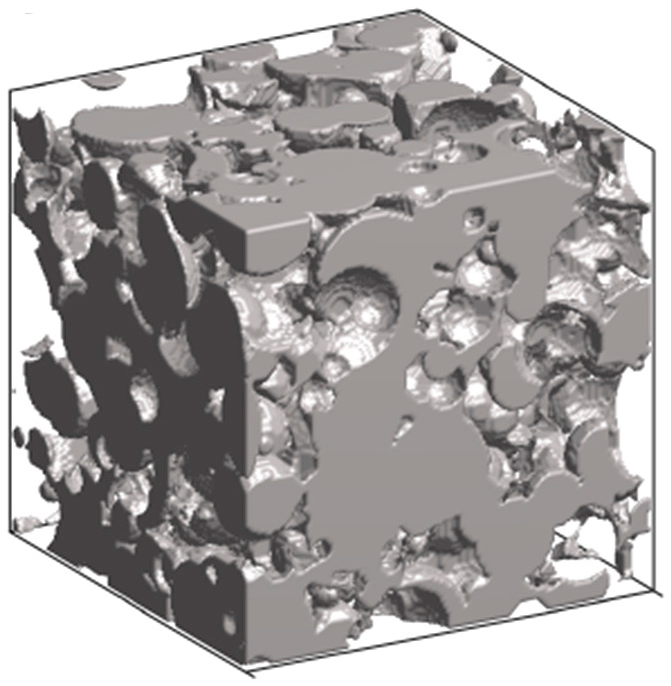
\includegraphics[width=0.45\textwidth]{../images/form_factor/nonparticular/dead_leaves_3D.png}
\end{center}
\caption{A real space realisation of a dead-leaves model \cite{Gommes2018}.} \label{fig:DeadLeaves3D}
\end{figure}

A dead-leaves model of porous material is obtained by randomly covering an
initially empty space by pore-like or solid-like spheres, and letting
them overlap so that only the topmost sphere is visible. The process has to be continued until the
entire space is covered either by pore-like or solid-like spheres.

For the dead leaves model the Debye correlation function is independent of the volume fraction of pores or particles and reads as
\begin{align}\label{eq:DebyeCorrelationDeadLeaves}
  \gamma(r) &= \frac{K_\mathrm{LN}(r)}{2K_\mathrm{LN}(0)-K_\mathrm{LN}(r)}
\end{align}

\begin{figure}[htb]
\begin{center}
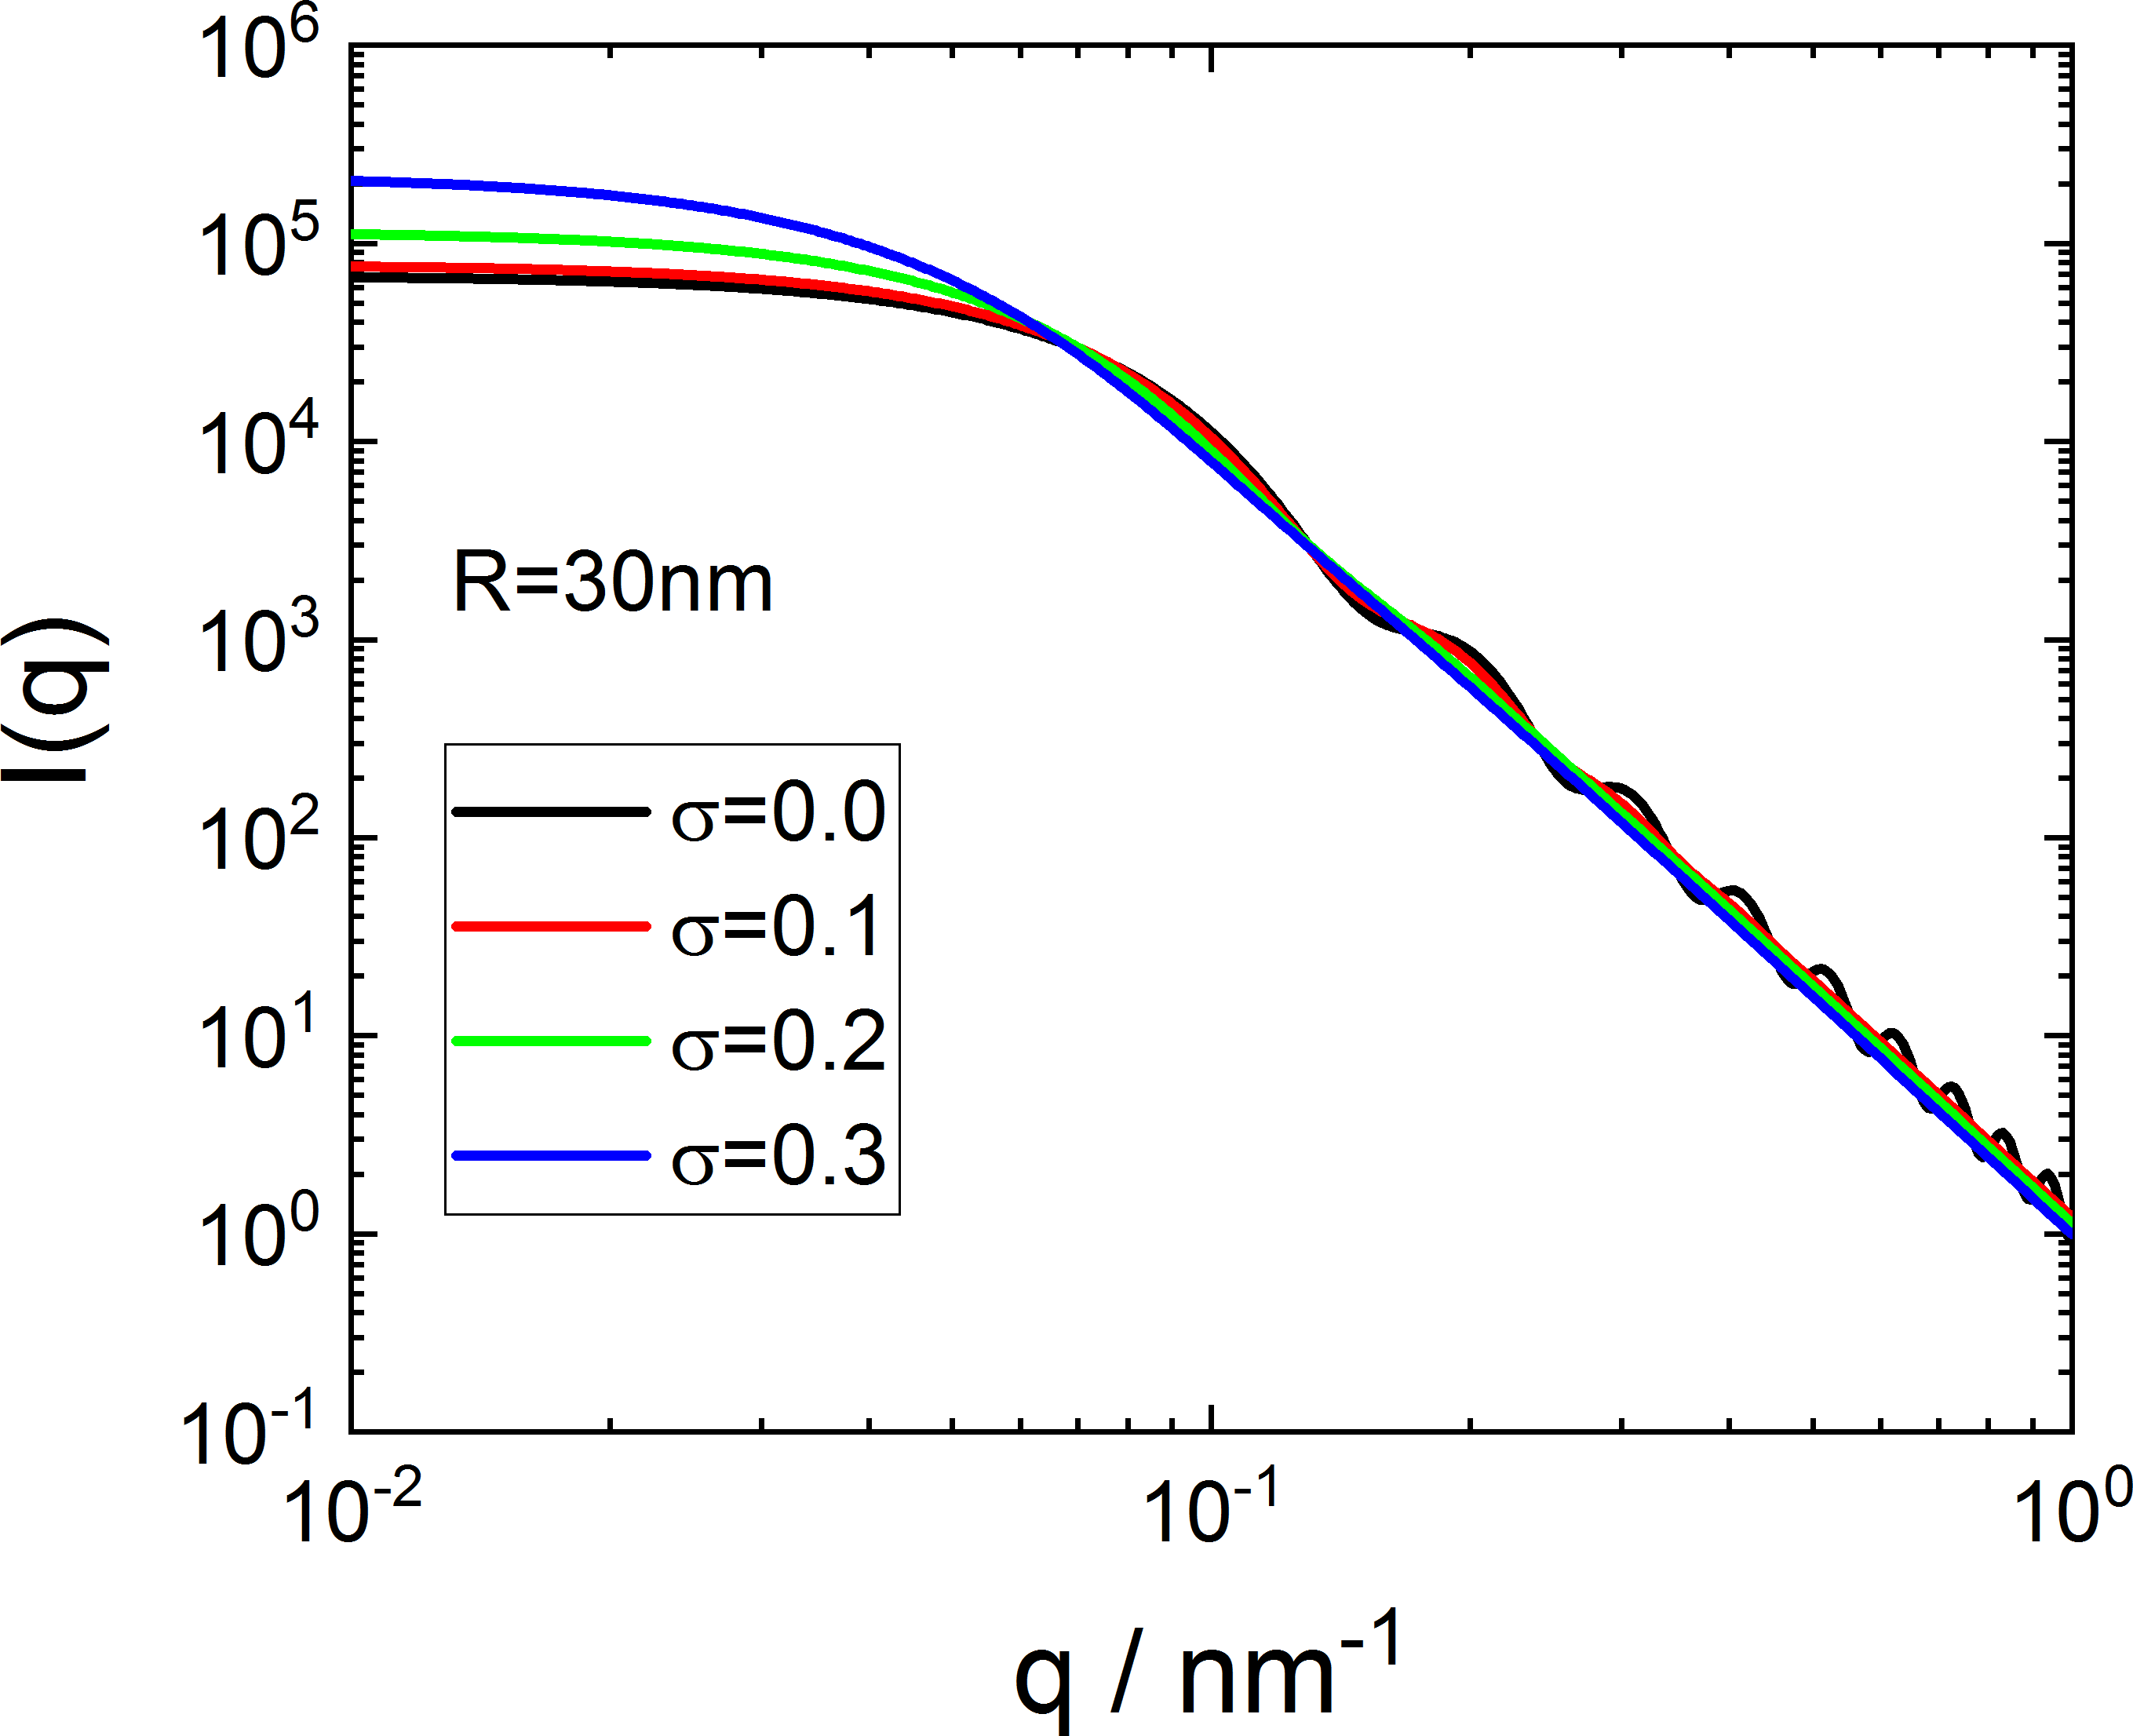
\includegraphics[width=0.45\textwidth]{../images/form_factor/nonparticular/dead_leaves.png}
\end{center}
\caption{Dead-leaves model for different size distributions} \label{fig:DeadLeavesIQ}
\end{figure}

\underline{Input Parameters for model \texttt{dead leaves model}:}\\
\begin{description}
\item[\texttt{scale}] characteristic length for positional correlation $\xi$
\item[\texttt{dummy}] not used
\item[\texttt{mu}] median $\mu$ of LogNorm distribution
\item[\texttt{sigma}] width $\sigma$ of LogNorm distribution
\end{description}

\vspace{5mm}

\underline{Note:}
\begin{itemize}
\item None
\end{itemize}


\newpage
\subsubsection{boolean (union model)}~\\

\begin{figure}[htb]
\begin{center}
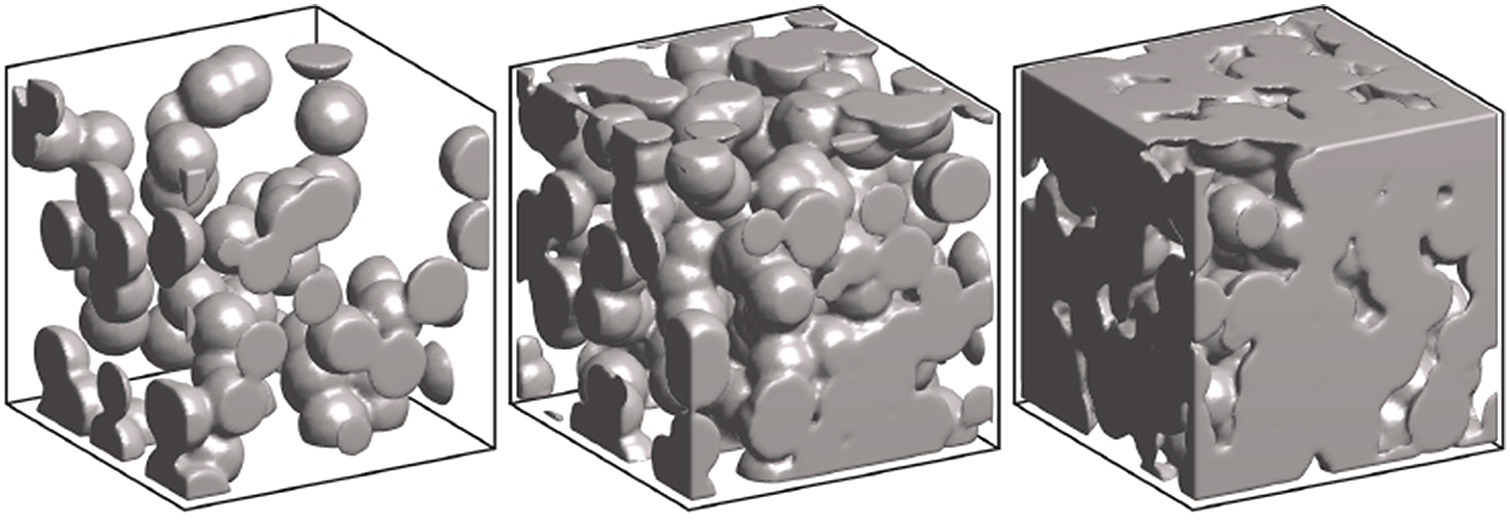
\includegraphics[width=0.85\textwidth]{../images/form_factor/nonparticular/boolean_union_3D.png}
\end{center}
\caption{A real space realisation of a boolean union model of monodisperse spheres for $\phi_1=0.2, 0.5$, and 0.8 (taken from \cite{Gommes2018}).} \label{fig:BooleanUnion3D}
\end{figure}

The Boolean (union model) the structure is described as random positioned overlapping solid-like grains. The pore centers are positioned following a Poisson point process with density $\theta$ (average number density of grains). In the implemented model the grains are assumed being spheres with a size distribution. The geometrical covariogram is given by eq.\ \ref{eq:covariogram_sphere_LogNorm}. The corresponding Debye correlation function is than given by
\begin{align}\label{eq:Debye_correlation_function_boolean_union}
  \gamma(r) &= \frac{\exp\left(\theta K_\mathrm{LN}(r)\right)-1}{\exp\left(\theta K_\mathrm{LN}(0)\right)-1} \\
            &= \frac{\exp\left(\theta K_\mathrm{LN}(r)\right)-1}{\frac{1}{\phi_0}-1}
\end{align}
where $\phi_0=1-\phi_1=\exp(-\theta K_\mathrm{LN}(0))$ is the volume fraction of pores.

\begin{figure}[htb]
\begin{center}
\subfigure[Effect of volume fraction, but monodisperse spheres]{
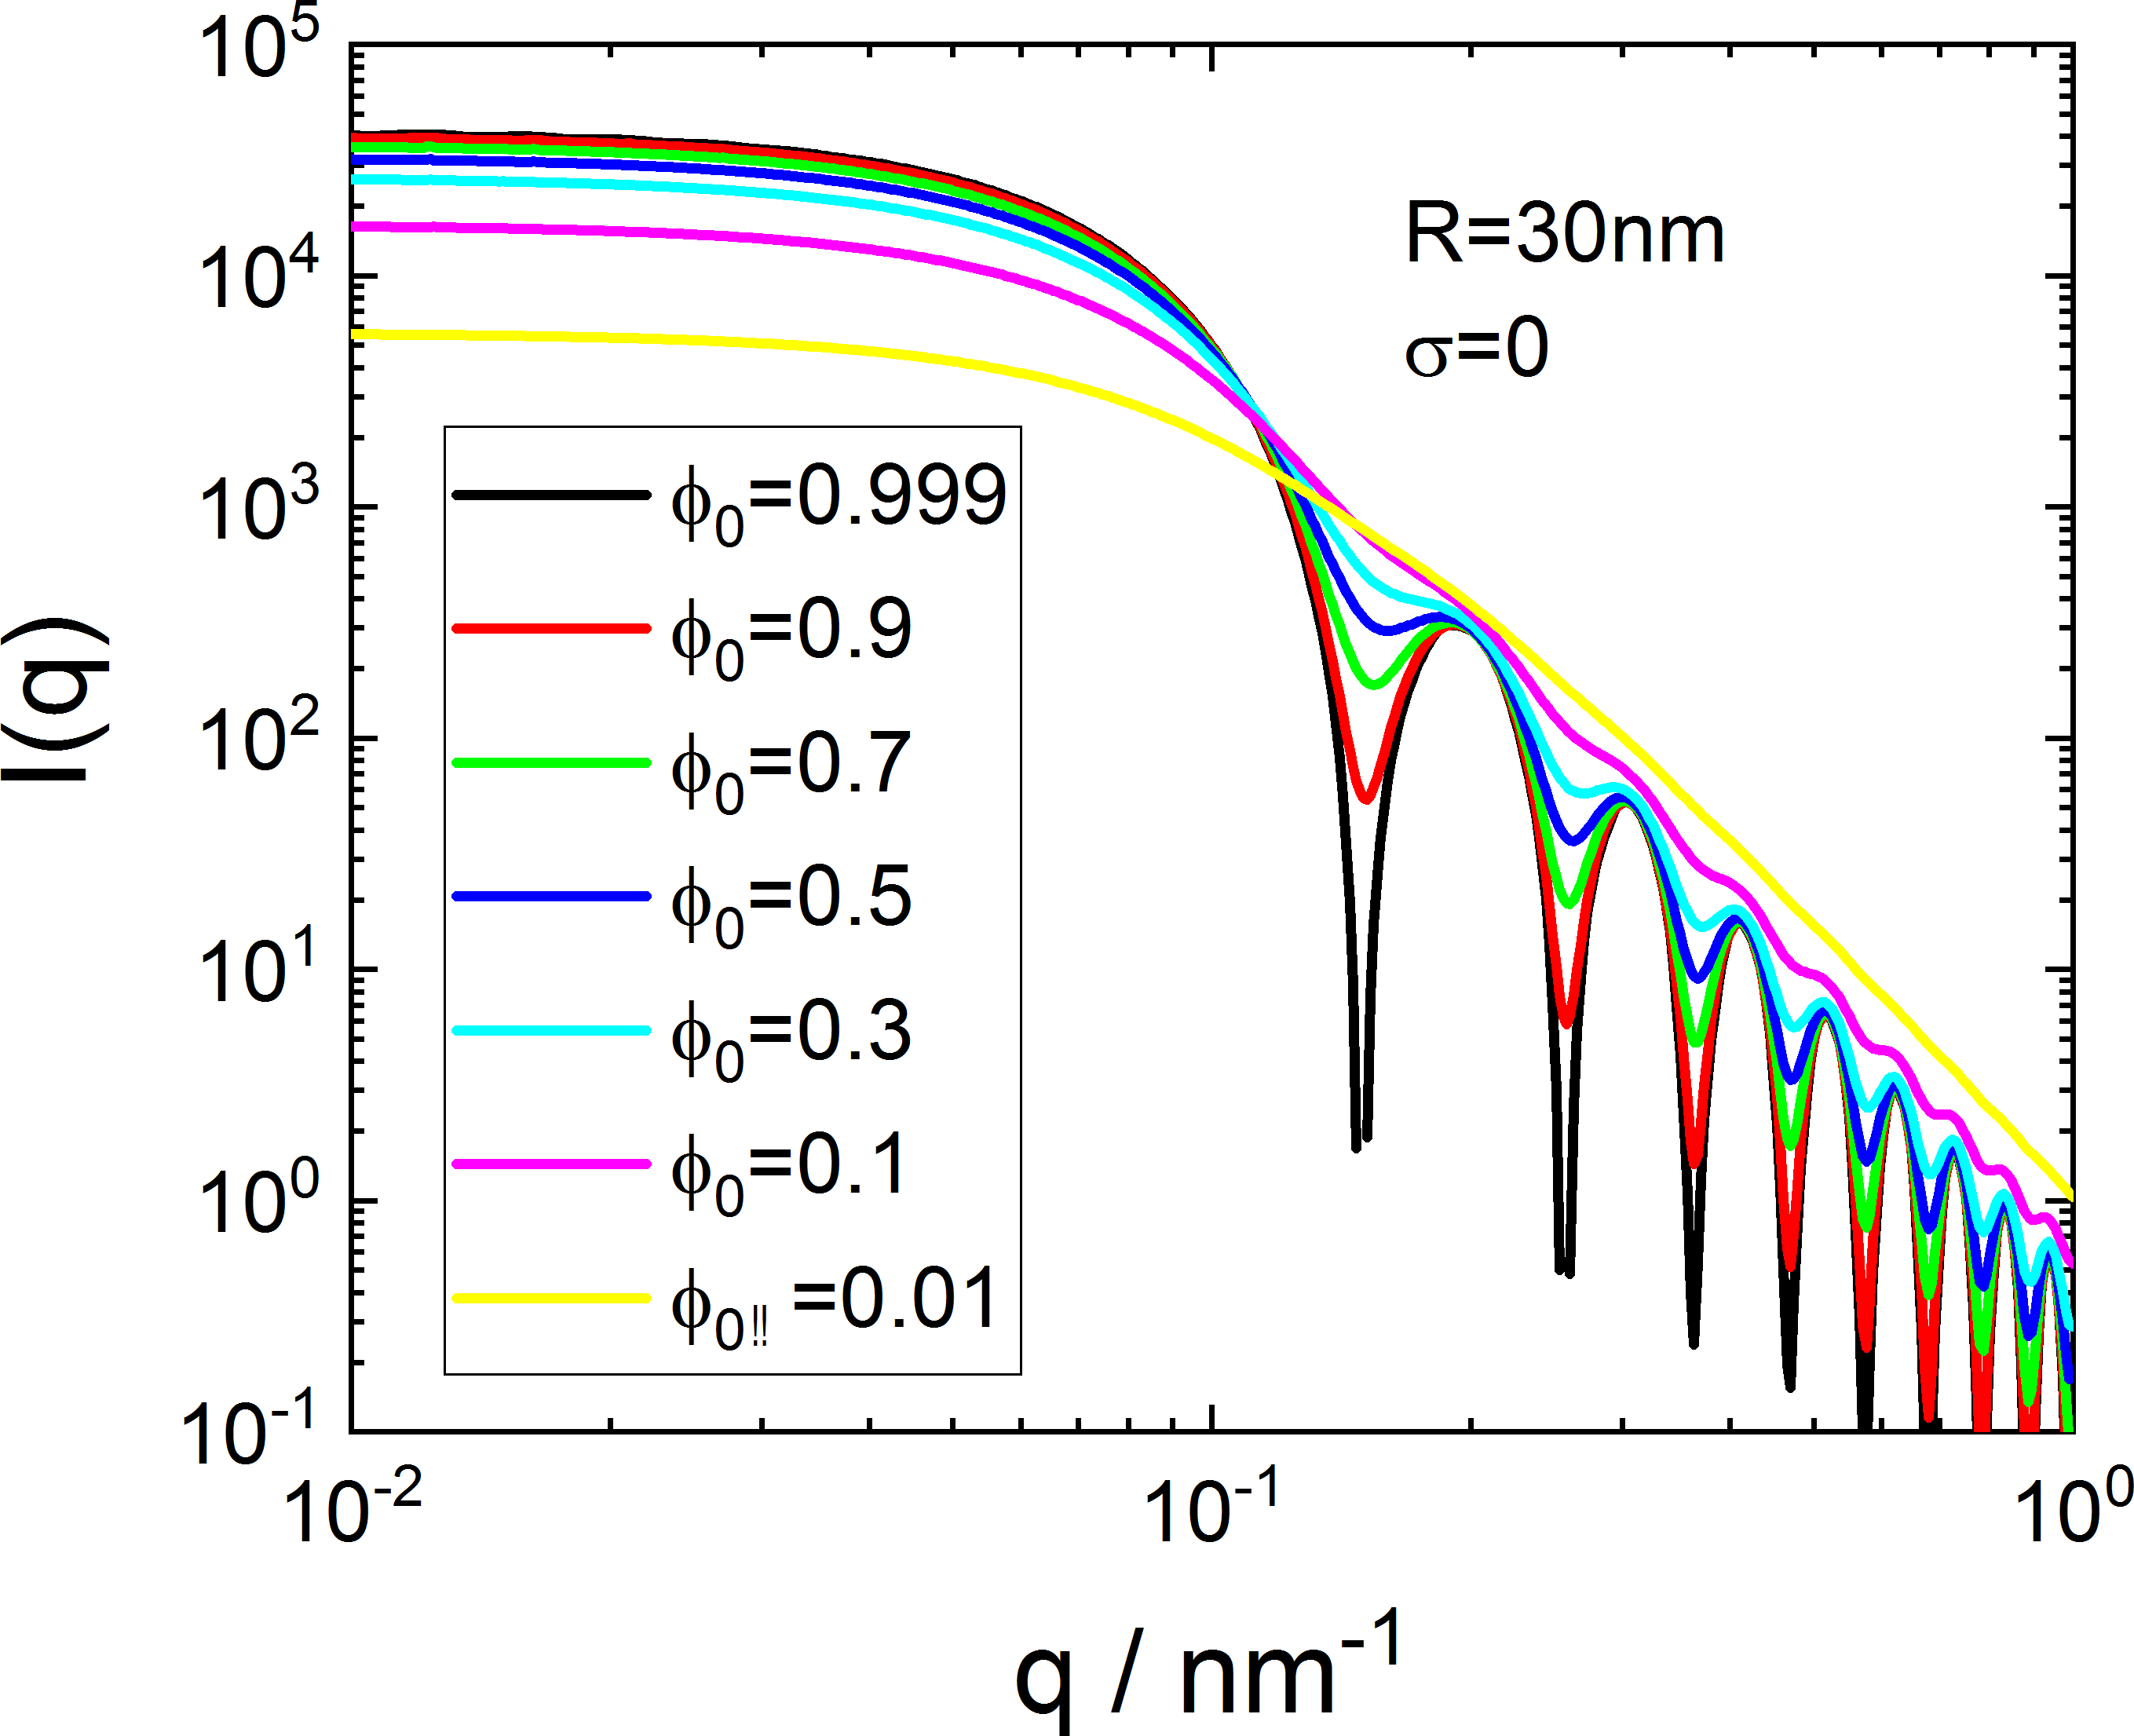
\includegraphics[width=0.48\textwidth]{../images/form_factor/nonparticular/BooleanUnionPhi0.png}}
\hfill
\subfigure[Effect of size distribution at fixed volume fraction $\phi_0=0.8$]{
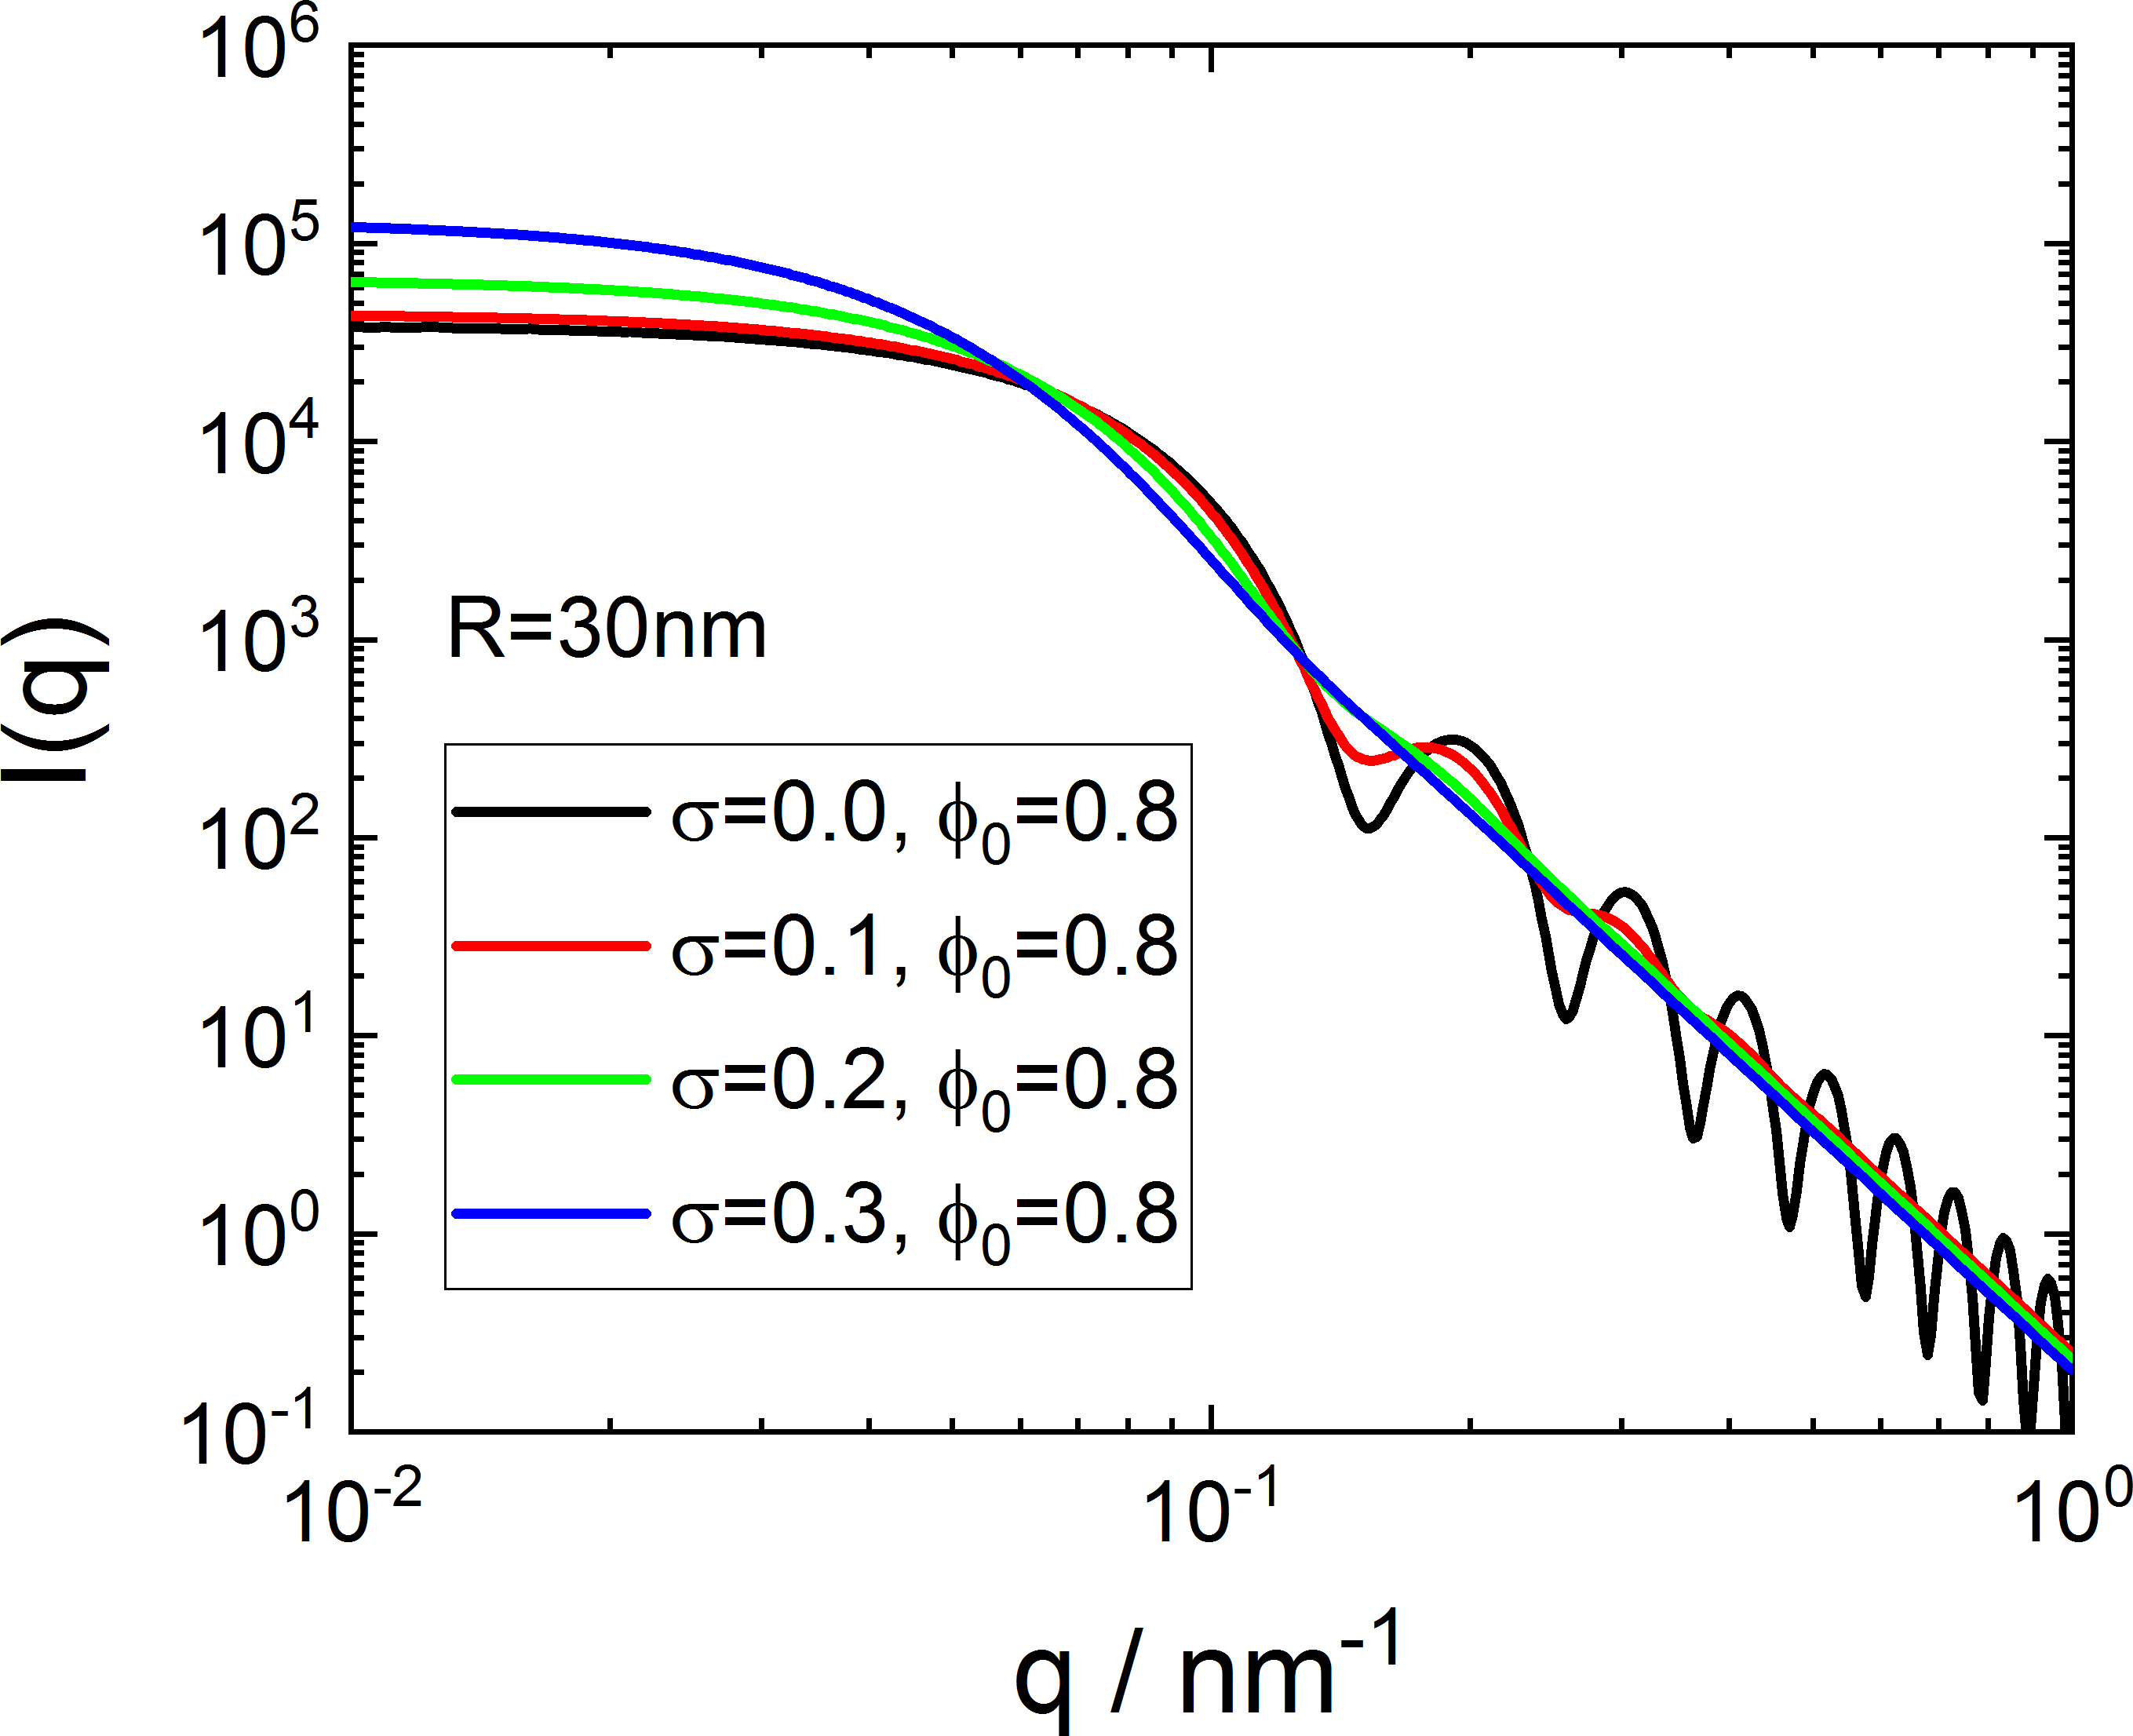
\includegraphics[width=0.48\textwidth]{../images/form_factor/nonparticular/BooleanUnionSigma.png}}
\end{center}
\caption{Boolean union model of spheres}
\label{fig:BooleanUnion}
\end{figure}


\underline{Input Parameters for model \texttt{boolean union model}:}\\
\begin{description}
\item[\texttt{scale}] characteristic length for positional correlation $\xi$
\item[\texttt{phi0}] volume fraction $\phi_0$ of pore-like phase
\item[\texttt{mu}] median $\mu$ of LogNorm distribution
\item[\texttt{sigma}] width $\sigma$ of LogNorm distribution
\end{description}

\vspace{5mm}

\underline{Note:}
\begin{itemize}
\item None
\end{itemize}

\newpage
\subsubsection{boolean (intersection model)}

\newpage
\subsubsection{clipped random fields} ~\\

Clipped random field model are mathematically formalized geometrical models which have been applied to small angle scattering e.g.\ by \cite{Berk1991,Teubner1991,Levitz1998,Roberts1995}. These class of models describe the morphology by stochastic standing wave $S(\mathbf{r})$ defined by
\begin{align}
S(\mathbf{r}) &= \frac{1}{\sqrt{N\langle A^2\rangle}} \sum_{n=1}^N A_n \cos\left(\mathbf{q}_n\cdot\mathbf{r}+\phi_n\right)
\end{align}
$\phi_n$ and $A_n$ are independent random variables, however the squared average amplitude need to be finite. For $N\rightarrow \infty$ the properties of $S(\mathbf{r})$ becomes independent of the distribution $A_n$ and are therefore assumed to be $A_n=1/\sqrt{2}$. The phase $\phi_n$ is assumed to be uniform distributed over $(0,2\pi)$ and the direction of the random wave vector $\mathbf{q}_n$ is uniformly distributed over all solid angle $4\pi$. The distribution of the length of the wave vectors however follow a distribution $f(q)$ (spectral function), which than determines the properties of $S(\mathbf{r})$. The distribution is normalized so that $\int_0^\infty f(q) \mathrm{d}q=1$ The scattering length density $\rho(\mathbf{r})$ than takes values of $\rho_1$ or $\rho_0$ depending if $S(\mathbf{r})$ is larger or smaller than a threshold $\alpha$, which can be written as
\begin{align}
  \rho(\mathbf{r}) & = (\rho_1-\rho_0) \Theta(S(\mathbf{r})-\alpha) + \rho_0
\end{align}
It is also possible to perform the definition via two thresholds $\alpha$ and $\beta$ between which the value of $S(\mathbf{r})$ has to lay to be assigned to $\rho_1$. An extension to a three phase system is also straight forward where then the phases are assigned according to the intervals $(-\infty,\alpha)$, $(\alpha,\beta)$, and $(\beta,\infty)$.
The two-point correlation function $g_S$ of an isotropic gaussian random field is
\begin{align}\label{eq:gr_CGRF}
  g_S(\mathbf{r}) &= g_S(r) = \langle S(\mathbf{r}) S(\mathbf{r}+\mathbf{x}) \rangle \\
                  &= \int_0^\infty f(q) \frac{\sin qr}{qr} 4\pi q^2 \mathrm{d}q
\end{align}

\paragraph*{\textbf{Single threshold:}} \phantom{M}\hspace{1pt} \\

For the single threshold model a two-phase system is described by a single threshold $\alpha$. The volume fraction $\phi_1$ of the solid phase with the scattering length density $\rho_1$ is than given by
\begin{align}\label{eq:volumefraction_alpha}
  \phi_1 & = \frac12 - \frac12\mathrm{erf}\left(\frac{\alpha}{\sqrt{2}}\right)
\end{align}
where $\mathrm{erf}$ is the error function and $\phi_0=1-\phi_1$ the porosity. The covariance $C_{11}(r)$ than is defined as the probability that two gaussian fields $S(\mathbf{r})$ and $S(\mathbf{r}+\mathbf{x})$ takes values larger than $\alpha$. Mathematically this is described equivalently by
\begin{align}
  C_{11}(r) &= \frac{1}{2\pi} \int_0^{\arcsin(g_S(r))} \exp\left[\frac{-\alpha^2}{1+\sin\theta}\right] \mathrm{d}\theta + \phi_1^2
\end{align}
The Debye correlation function is than given by
\begin{align}
  \gamma(r) &= \frac{C_{11}(r) -\phi_1^2}{\phi_1\phi_0}
\end{align}
from which the scattering intensity can be calculates as
\begin{align}
  I_Q(q) &= \frac{1}{(2\pi)^3}\int_0^\infty \gamma(r) \frac{\sin qr}{qr} 4\pi r^2 \mathrm{d}r
\end{align}

\paragraph*{\textbf{Two-cut model:}}\hspace{1pt} \\
In the two-cut model, a solid phase is assumed where the random field has values between $-\alpha$ and $\alpha$
\begin{align}
  \rho(\mathbf{r}) & = (\rho_1-\rho_0) \Theta(S(\mathbf{r})-\alpha) \Theta(\alpha-S(\mathbf{r}))+ \rho_0
\end{align}
 The volume fraction $\phi'_1$ of the solid phase with the scattering length density $\rho_1$ is then given
by
\begin{align}\label{eq:Phi_1_twocut}
  \phi'_1 &= \mathrm{erf} \left( \frac{\alpha}{\sqrt{2}}\right)
\end{align}
The covariance $C'_{11}(r)$ is defined as the probability that two gaussian fields S(r) and S(r+x) takes values
between $\pm \alpha$ which is equivalent to
\begin{align}\label{eq:C11twocut}
  C'_{11}(r) &= \frac{1}{\pi} \int_0^{\arcsin(g_S(r))} \exp\left[\frac{-\alpha^2}{1+\sin\theta}\right] + \exp\left[\frac{-\alpha^2}{1-\sin\theta}\right]\mathrm{d}\theta + (\phi'_1)^2
\end{align}

\hspace{1pt} \\
\paragraph*{Two-cut intersection model:}\hspace{1pt} \\
In case of a two-cut intersection model one assumes that two independent clipped random fields with the same power spectrum must intersect to form the final structure. Therefore the probabilities have to be multiplied and the solid phase volume fraction is given by
\begin{align}\label{eq:Phi_1_twocutintersection}
  \phi_1 &=  \left(\phi'_1\right)^2
\end{align}
and
\begin{align}\label{eq:C11twocut}
  C_{11}(r) &=  \left(C'_{11}(r)\right)^2
\end{align}

To calculate the scattering intensity $I_Q(q)$ the spectral function $f(q)$ is assumed to be known as a parameterised function as well as its Fourier transformation, i.e. the two-point correlation function $g_S(r)$. In \SASfit four parametrisation of the two-point correlation function $g_S(r)$  have been implemented, a simplified two parameter function $ g_{S,1}(r;\xi,d)$ \cite{Gommes2008,Gommes2018} and three 3-parameter functions. For this see e.g. \cite{Quintanilla2003,Roberts1997} $g_{S,2}(r;\xi,d,r_c)$ and \cite{Pieruschka1992} $g_{S,3}(r;\xi,d,r_c)$, \cite{Jinnai2000} $ g_{S,4}(r;\xi,d,r_c)$, or \cite{Chen1998}  $g_{S,5}(r;\xi,d,r_c)$.
\begin{align}
  g_{S,1}(r;\xi,d)    &= \frac{1}{\cosh(r/\xi)}\frac{\sin (2\pi r/d)}{2\pi r/d}\\
  g_{S,2}(r;\xi,d,r_c) &= \frac{\exp(-r/\xi)-r_c/\xi \exp(-r/r_c)}{1-r_c/\xi} \frac{\sin (2\pi r/d)}{2\pi r/d}\\
\begin{split}
 g_{S,3}(r;\xi,d,r_c) &= \frac{\sin (2\pi r/d)}{2\pi r/d} \frac{\frac{\xi}{r_c}\left(\frac{\xi}{r_c}+1\right)}{\left(\frac{\xi}{r_c}-1\right)^2}  \\
     & \left(e^{-r/\xi}+\frac{r_c}{\xi}e^{-r/r_c} - \frac{4\xi\left(e^{-r/\xi}-e^{-r/r_c}\right)}{r\left(\frac{\xi^2}{r_c^2}-1\right)}\right)
\end{split} \\
\begin{split}
  g_{S,4}(r;\xi,d,r_c) &= \frac{4bc\left(a^2+\left(b+c\right)^2\right)^2}{(b+c)r}  \\
                      & \times \Bigg[ e^{-cr}\Bigg(\frac{a^2-b^2+c^2}{\left(4a^2b^2+\left(a^2-b^2+c^2\right)^2\right)^2} \\
                      & + \frac{r}{4c\left(\left(a^2+b^2\right)^2+2\left(a^2-b^2\right)c^2+c^4\right)}\Bigg) \\
                      & +\frac{e^{-br}}{ab} \Bigg( \frac{-8a^2b^2+\left(a^2+b^2\right)^2+2\left(a^2-b^2\right)c^2+c^4}{4\left(4a^2b^2+\left(a^2-b^2+c^2\right)^2\right)^2}\\
                      & \times \sin(ar) - \frac{ab\left(a^2-b^2+c^2\right)}{\left(4a^2b^2+\left(a^2-b^2+c^2\right)^2\right)^2}\cos(ar)\Bigg) \Bigg]
\end{split} \\
\begin{split}
  g_{S,5}(r;\xi,d,r_c) &= \frac{1}{a^2+(c-b)^2} \Biggl\{ (a^2+c^2-b^2)\frac{\sin (ar)}{ar} \exp(-br)  \\
                      & +  2b \frac{\exp(-cr)-\exp(-br)\cos(ar)}{r}\Biggr\}
\end{split}
\end{align}
where $a=2\pi/d$, $b=1/\xi$, and $c=1/r_c$. Here $d$ is the quasi-periodic distance responsible for the peak in the scattering data and $\xi$ the decay length of that periodic structure, responsible for the width and height of the peak. The parameter $r_c$ controls for the 2nd and 3rd model the transition to the large $q$-values a bit, whereas in the 4th and 5th model it also has a big influence at small $q$-value below the peak position given by $d$.

\begin{figure}[htb]
\centering
  \subfigure[$r_c=80$nm]{\label{fig:rm80m}
     \begin{minipage}[b]{.45\linewidth}
             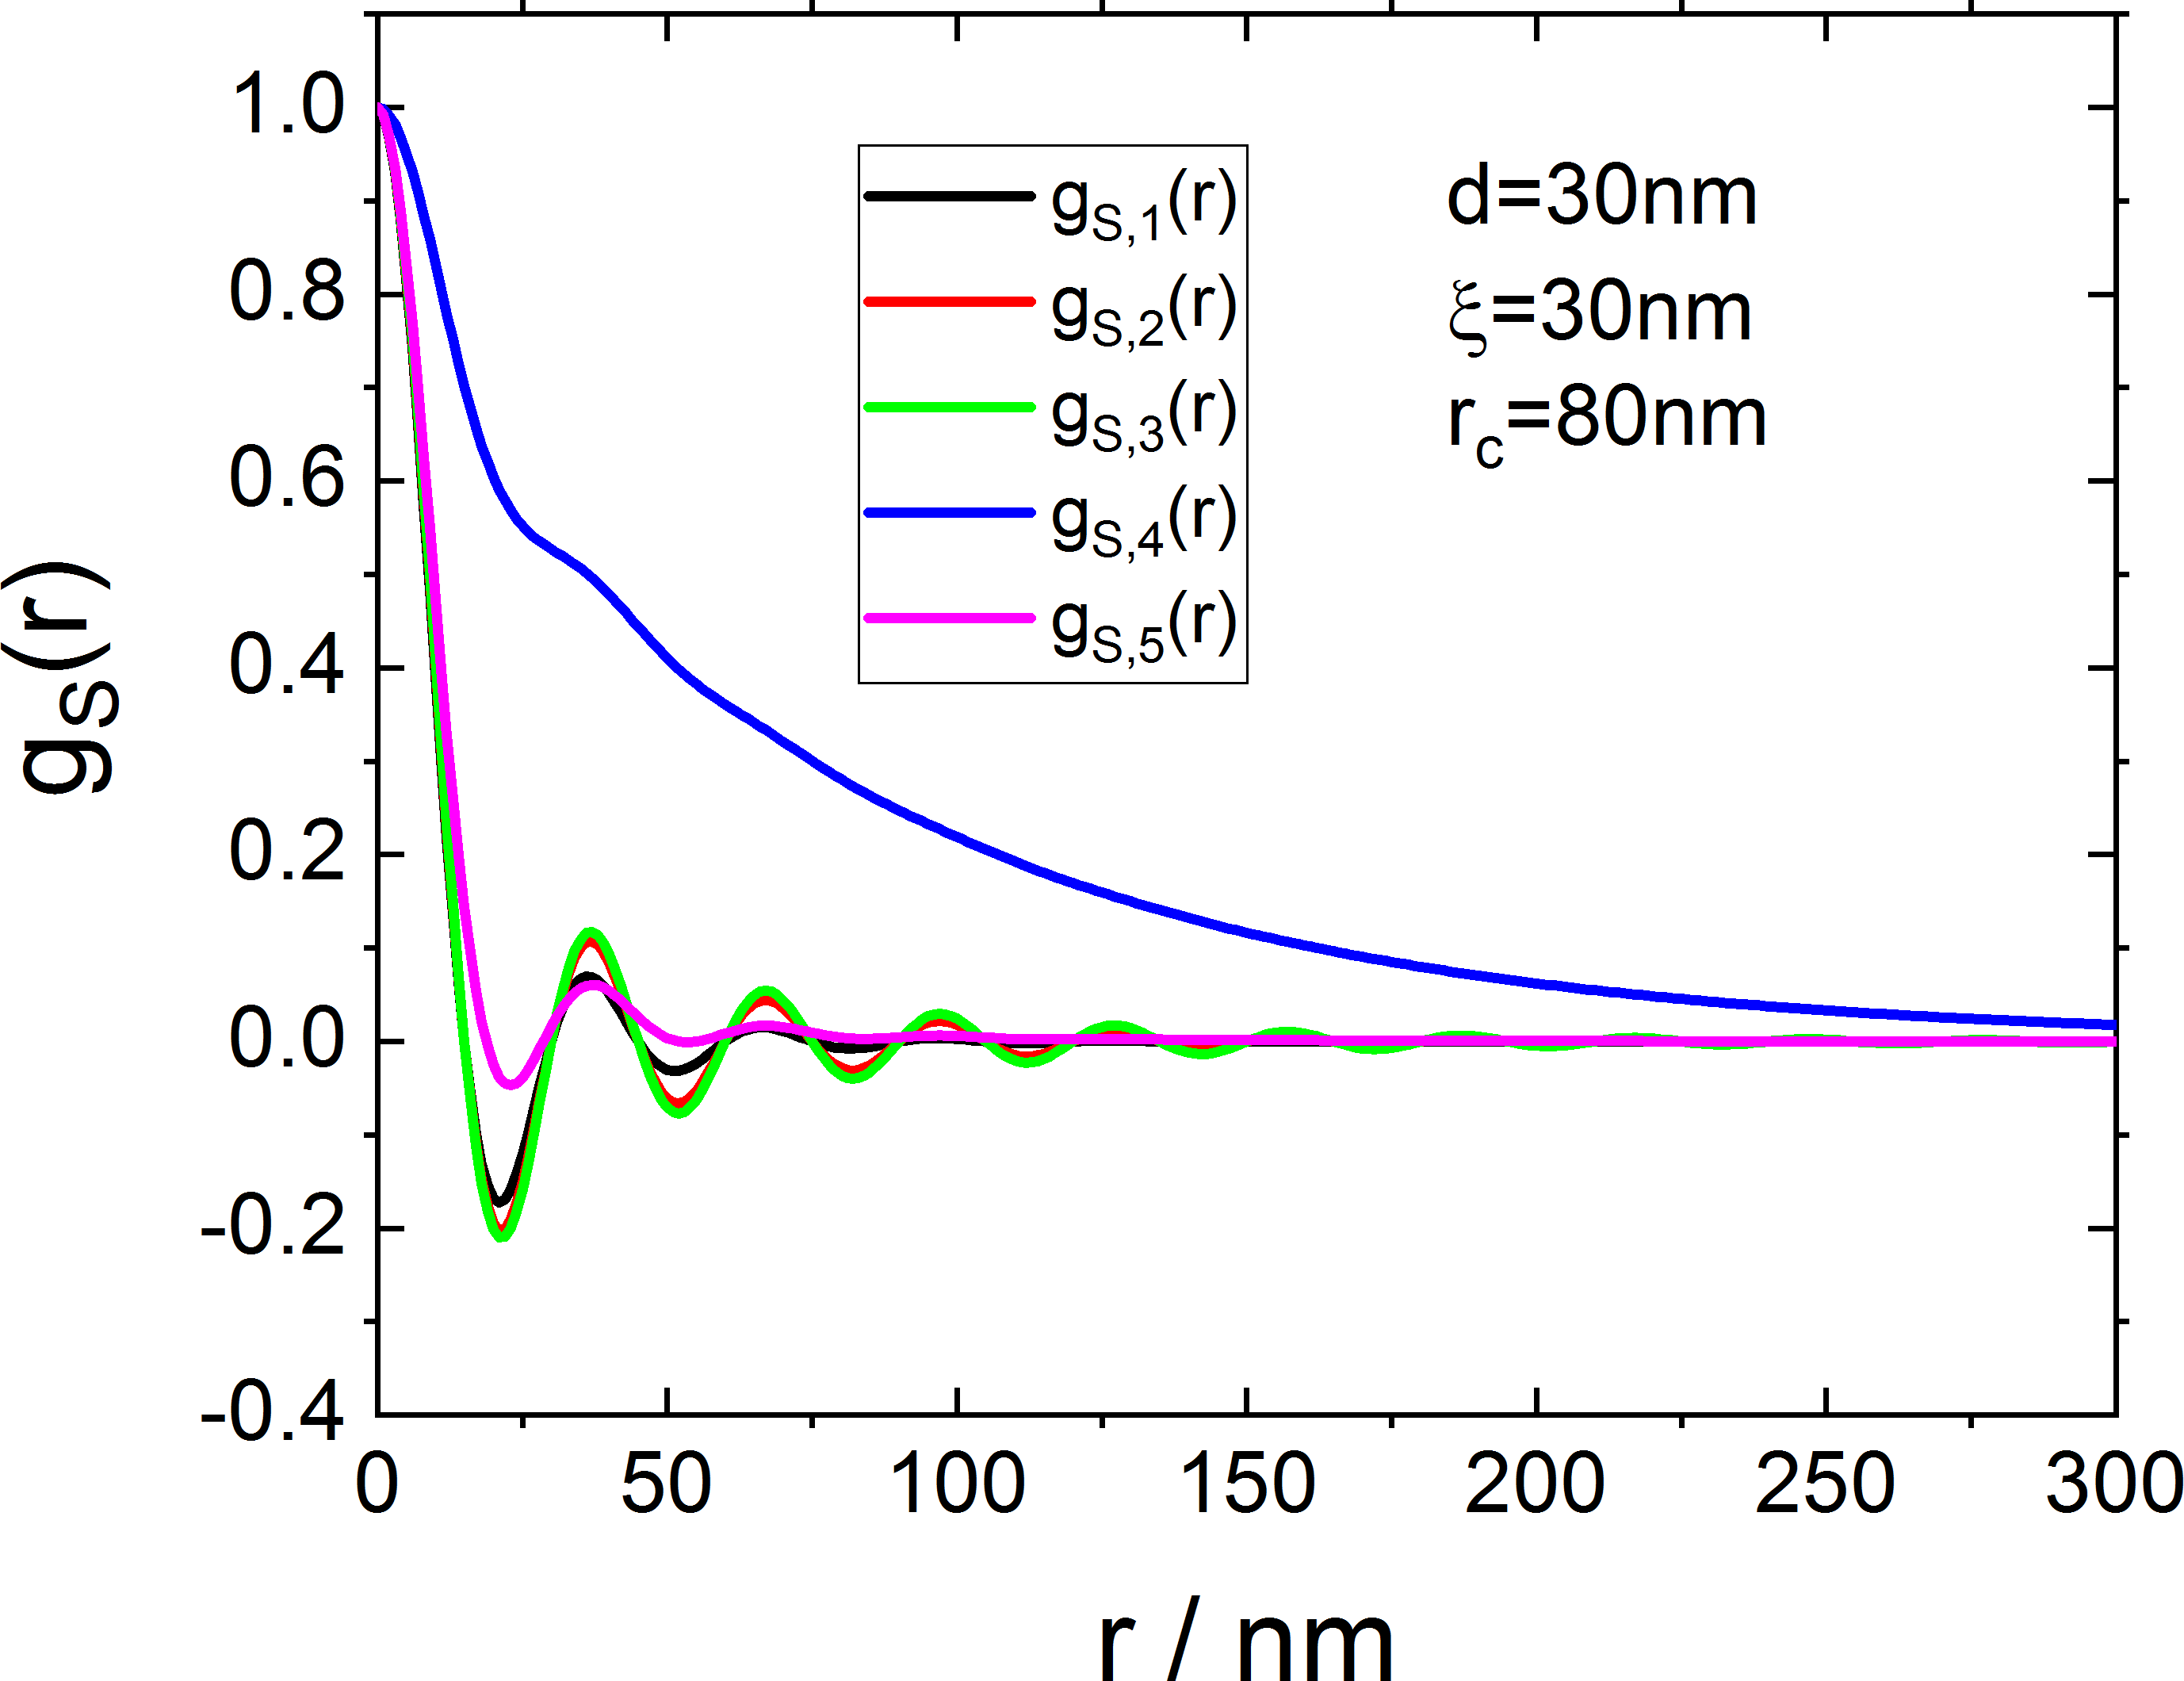
\includegraphics[width=1\linewidth]{../images/form_factor/nonparticular/gyr0_80.png}\\~\\
             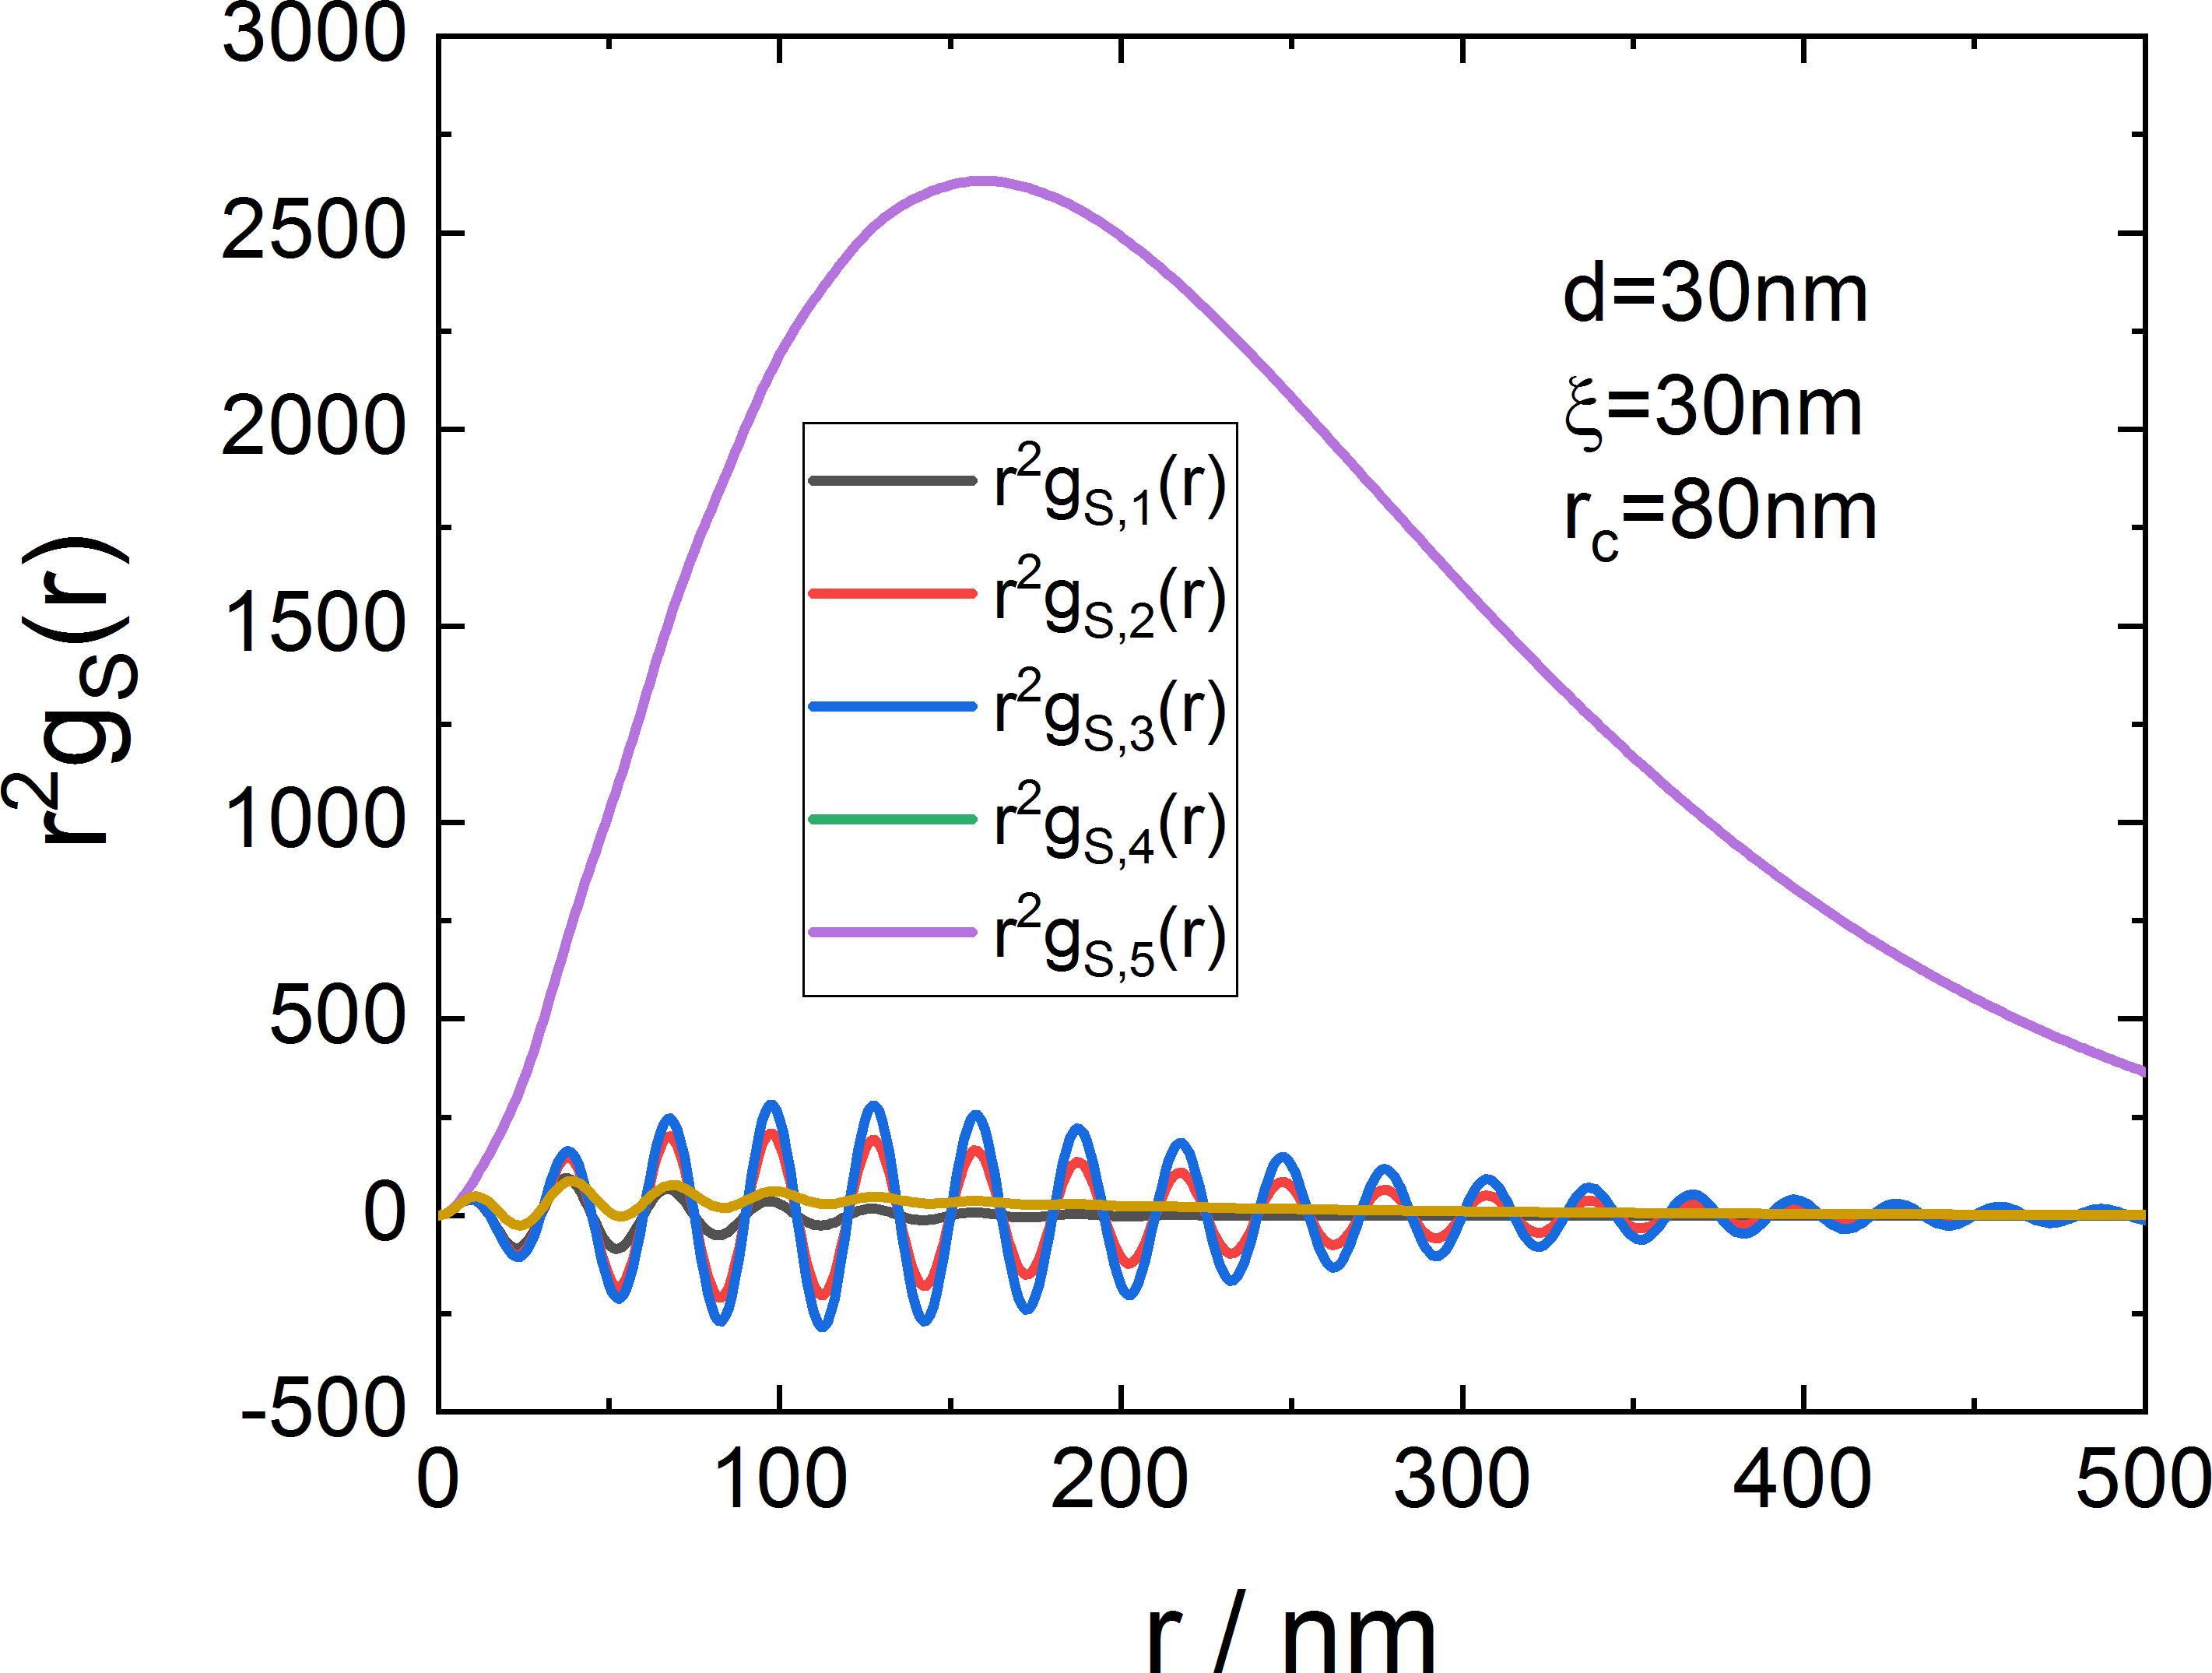
\includegraphics[width=1\linewidth]{../images/form_factor/nonparticular/gyr2_80.png}\\~\\
             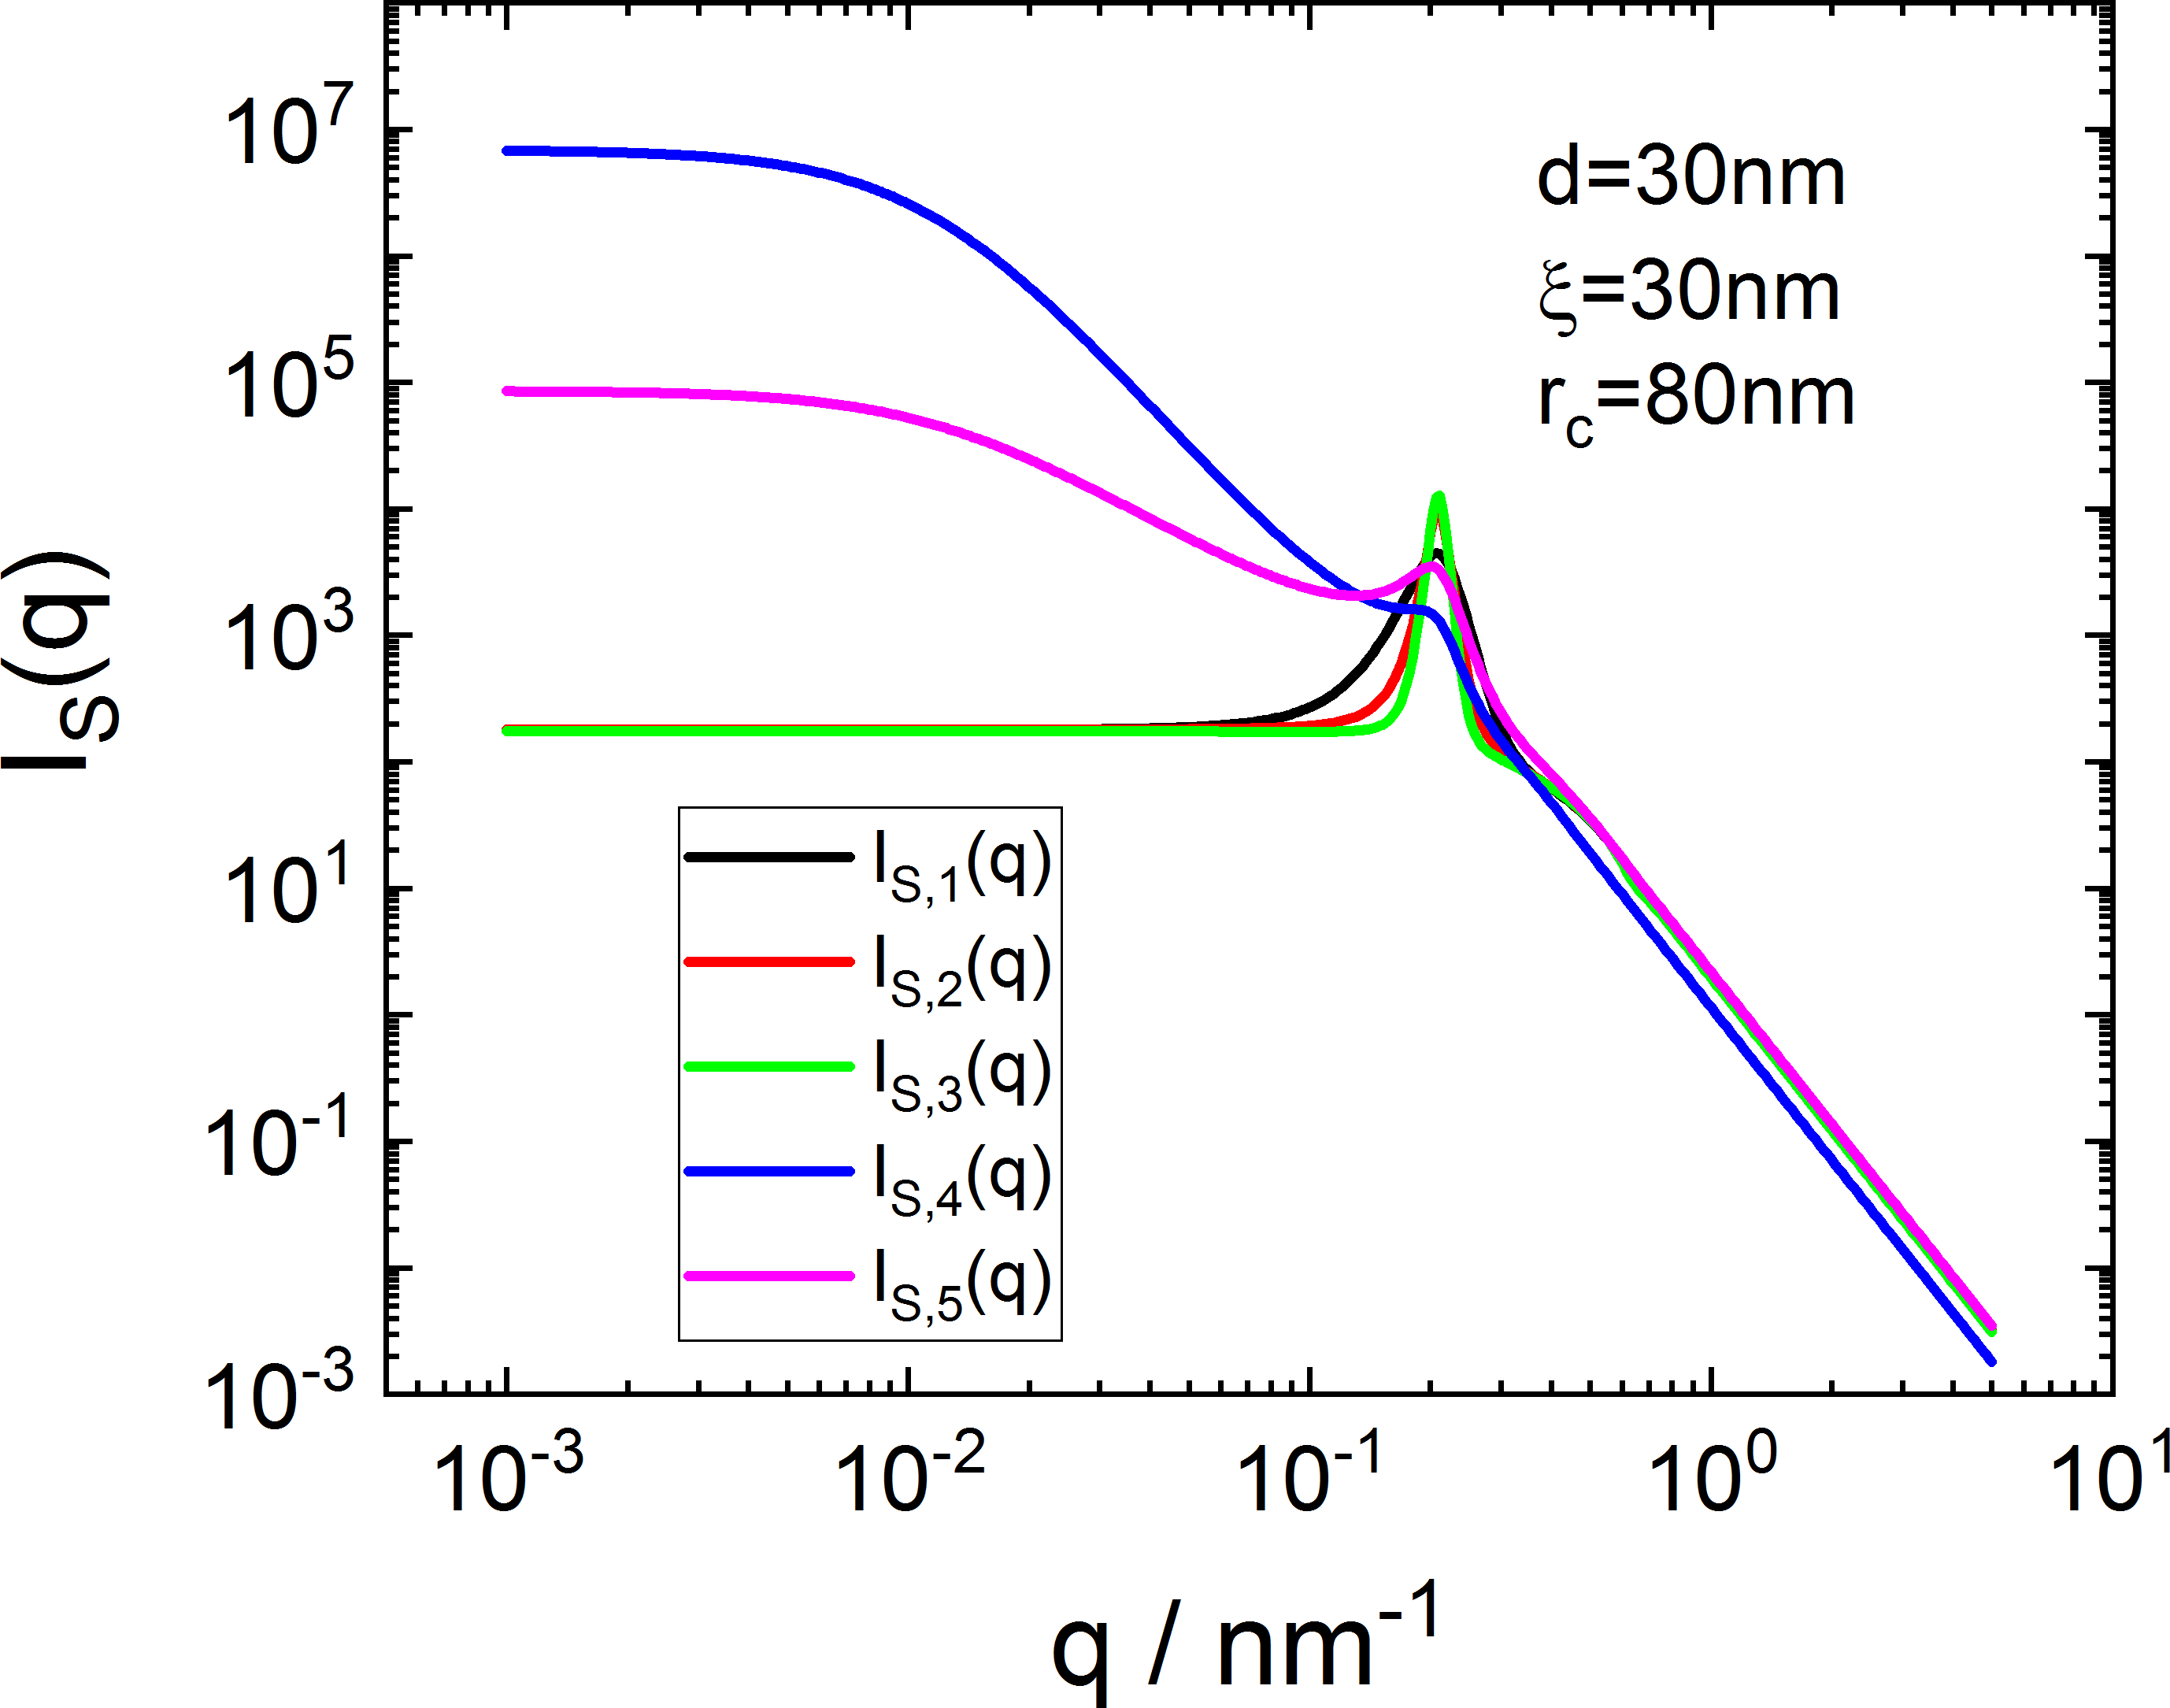
\includegraphics[width=1\linewidth]{../images/form_factor/nonparticular/IQCRW_80.png}
     \end{minipage}
     }
  \subfigure[$r_m=10$nm]{\label{fig:rm10nm}
    \begin{minipage}[b]{.45\linewidth}
             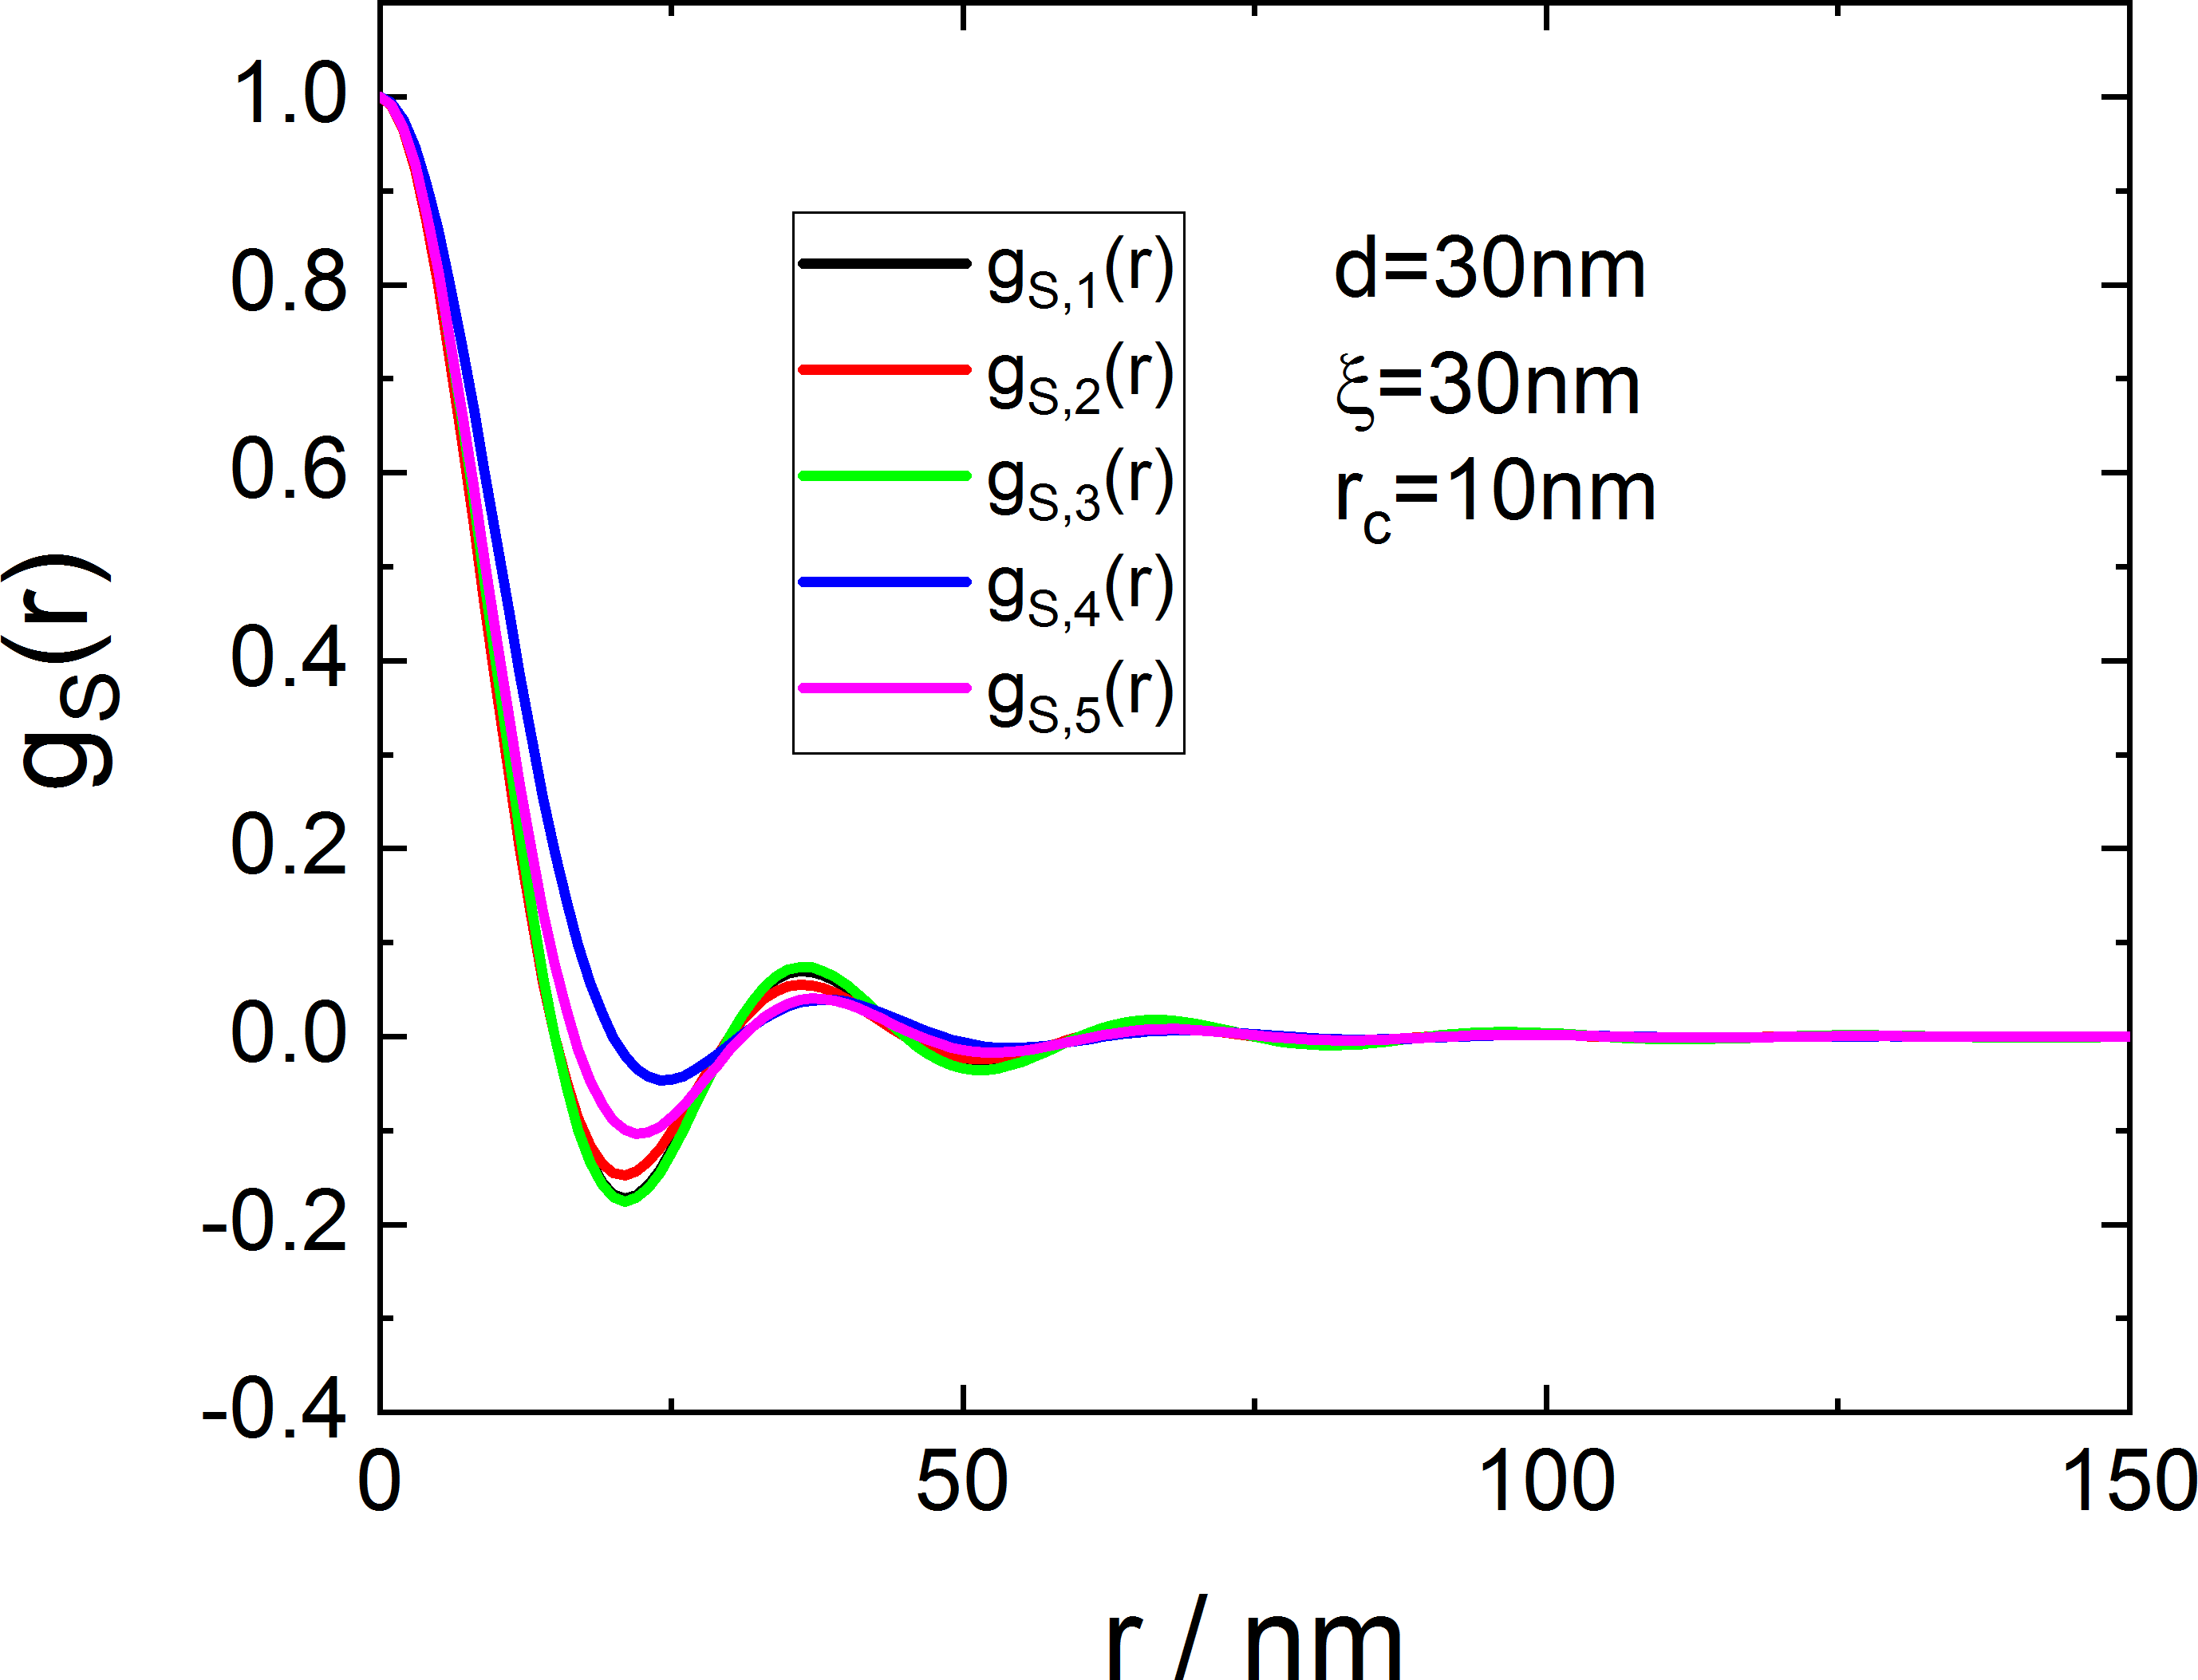
\includegraphics[width=1\linewidth]{../images/form_factor/nonparticular/gyr0_10.png}\\~\\
             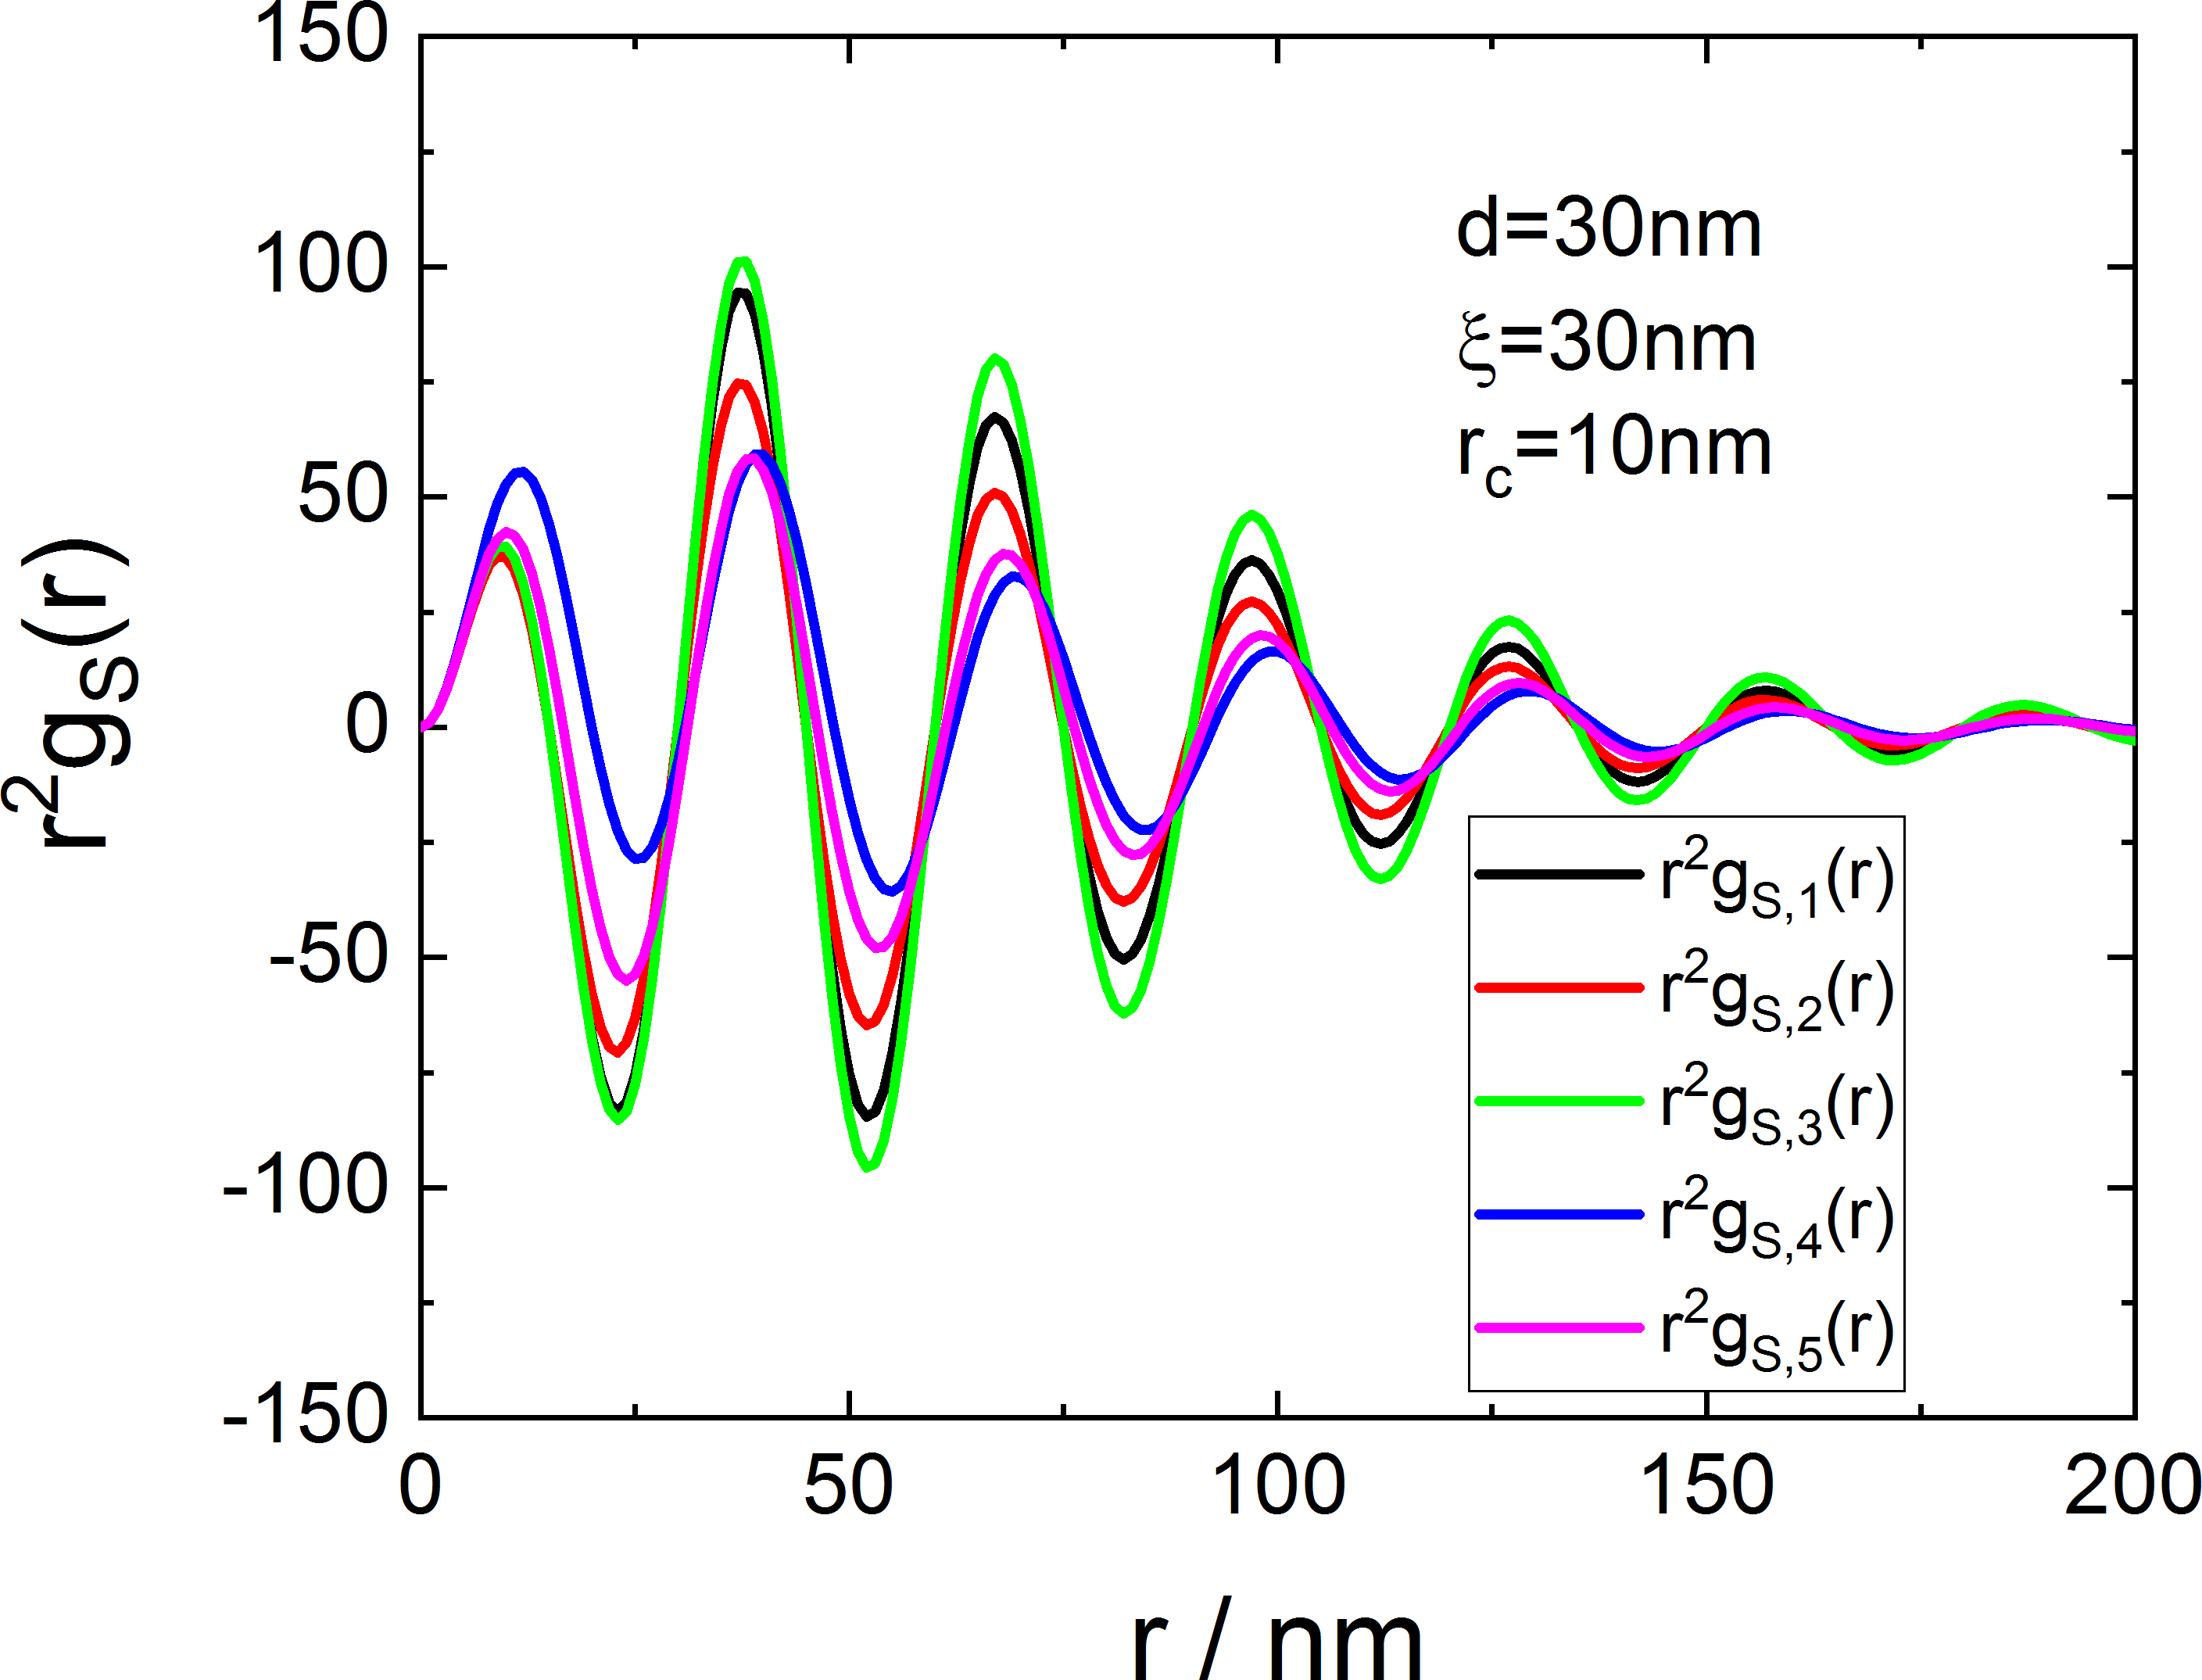
\includegraphics[width=1\linewidth]{../images/form_factor/nonparticular/gyr2_10.png}\\~\\
             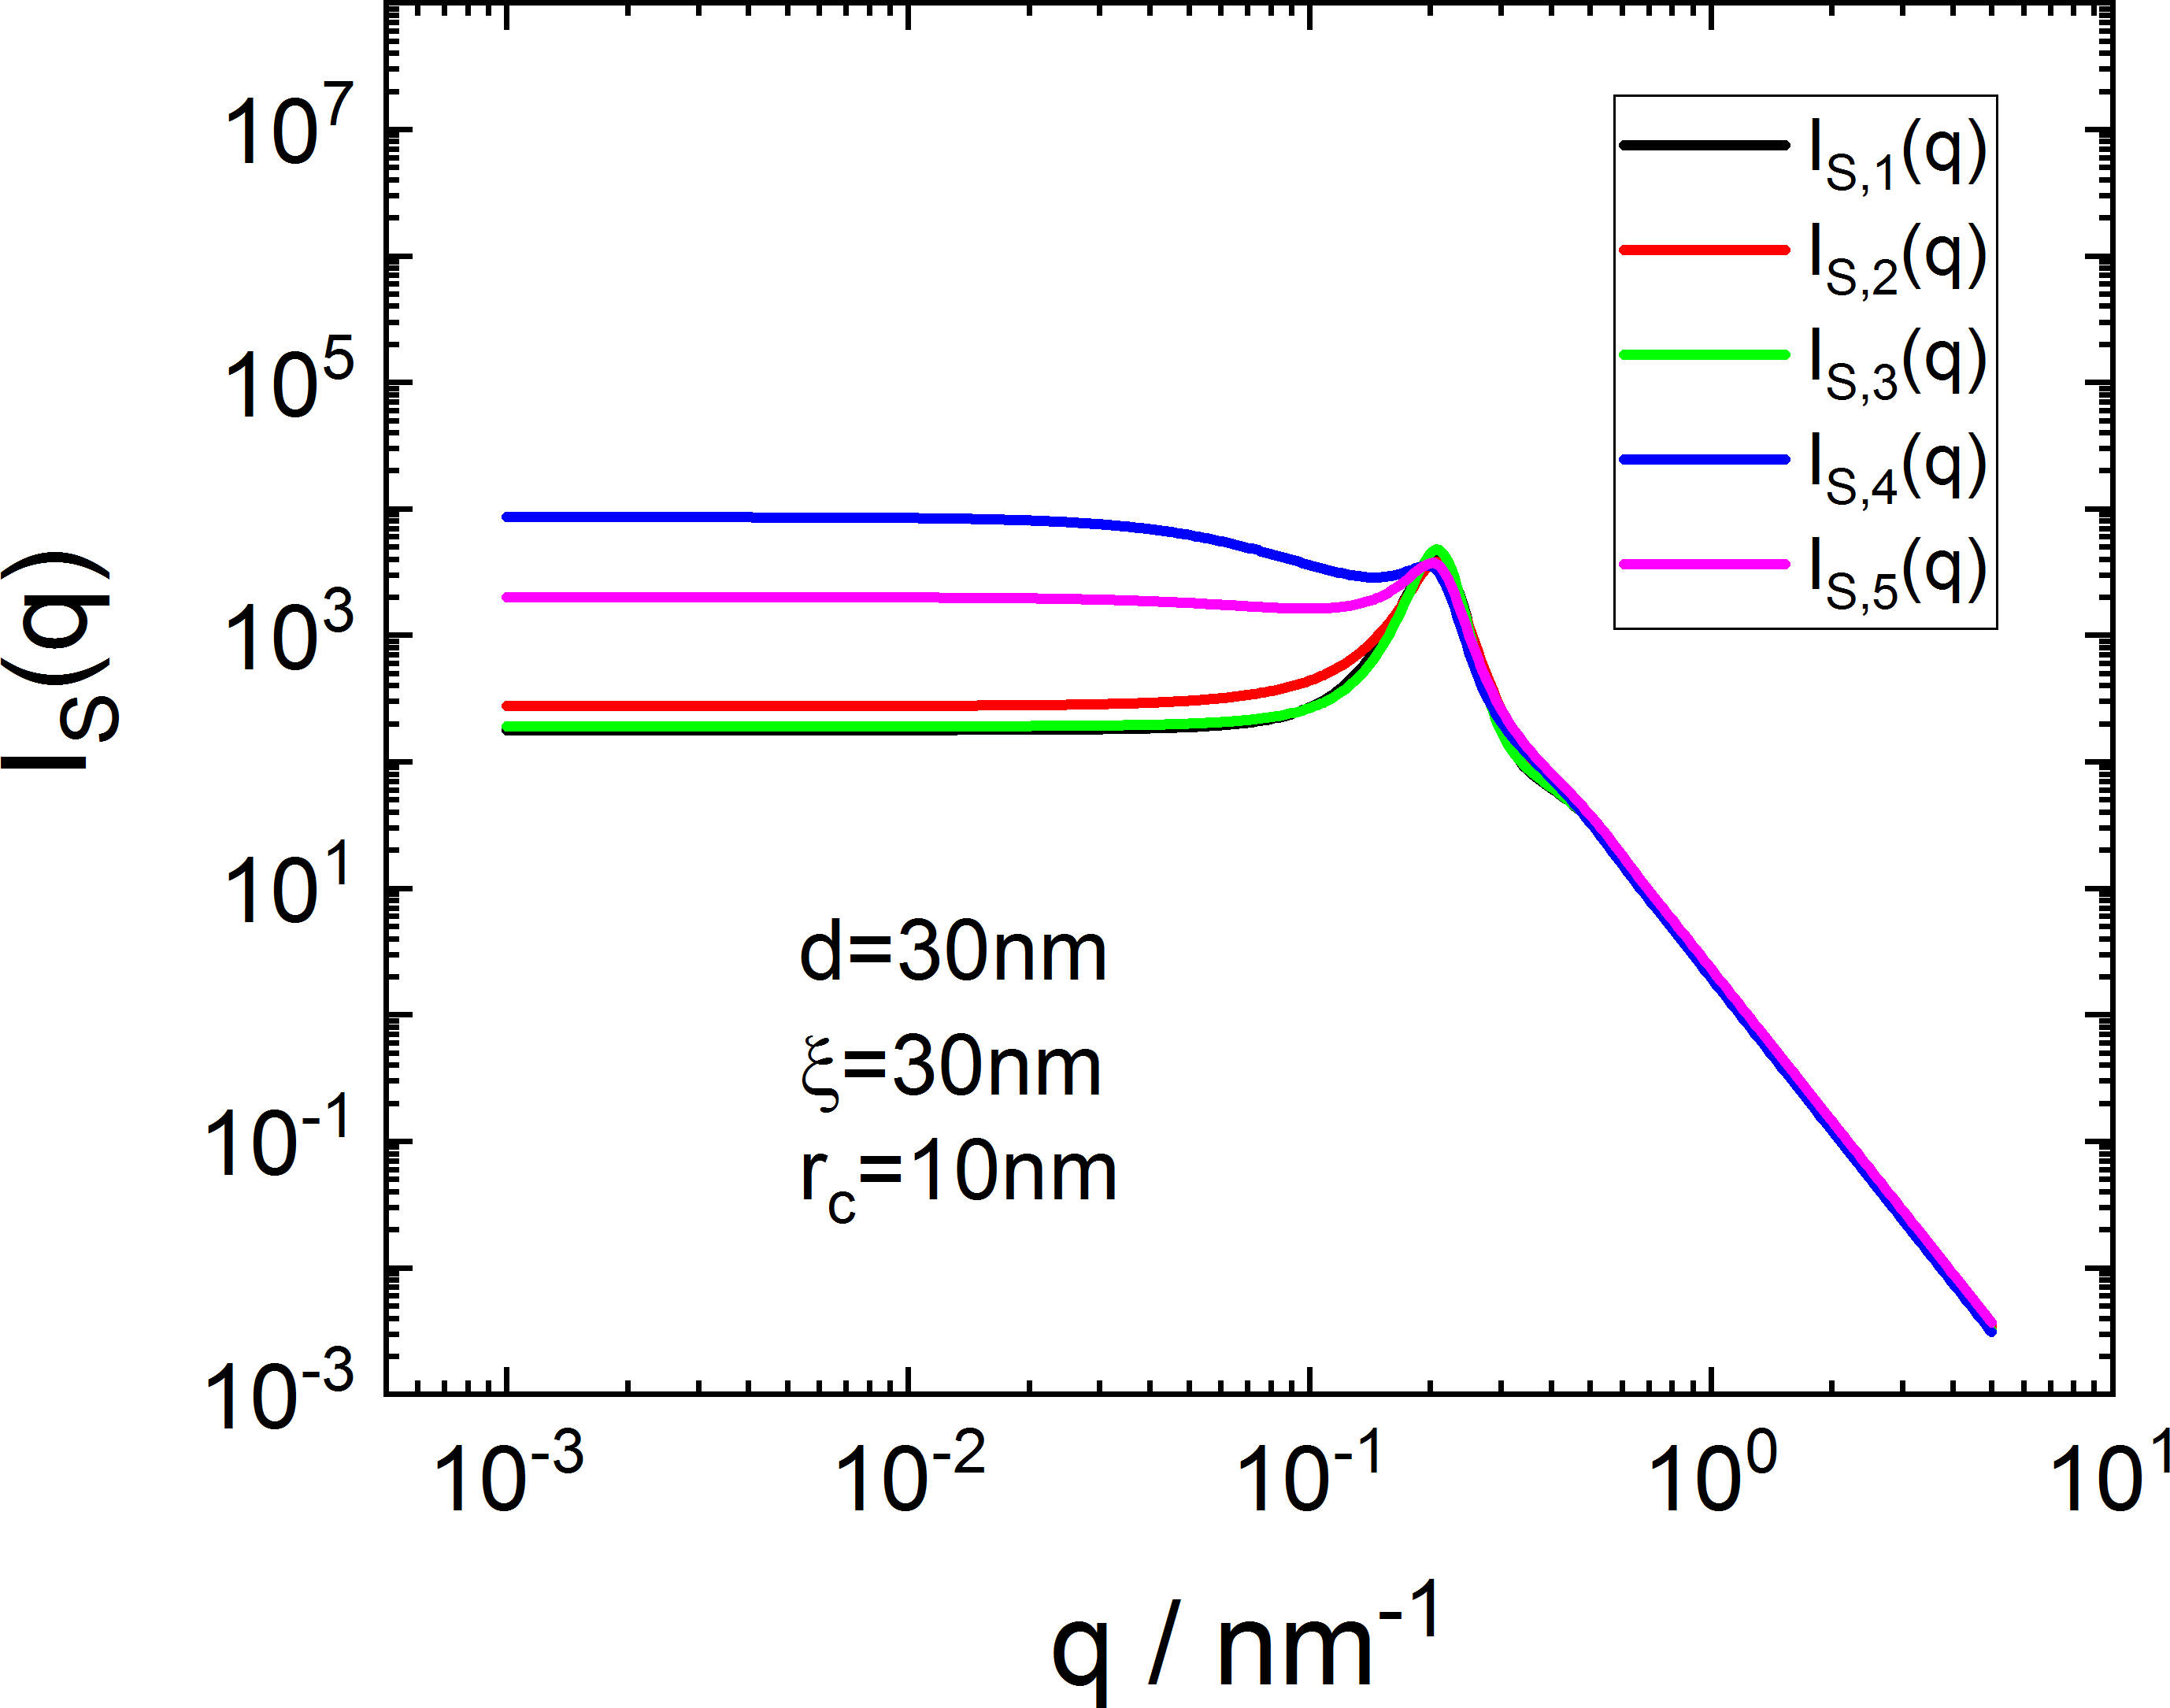
\includegraphics[width=1\linewidth]{../images/form_factor/nonparticular/IQCRW_10.png}
    \end{minipage}
    }
\caption{Two-point correlation functions $g_{S,1}\ldots g_{S,5}$ and corresponding scattering intensities $I_{S,1}(q)\ldots I_{S,5}(q)$} \label{fig:CRWplugin}
\end{figure}

\vspace{5mm}

\underline{Input Parameters for model \texttt{CRW 1}:}
\begin{description}
\item[\texttt{scale}] scaling factor for the intensity
\item[\texttt{d}] quasi-periodic distance $d$
\item[\texttt{xi}] decay length $\xi$ of that periodic structure
\end{description}

\vspace{5mm}

\underline{Input Parameters for models \texttt{CRW 2}, \texttt{CRW 3}, \texttt{CRW 4}, \texttt{CRW 5}:}\\
\begin{description}
\item[\texttt{scale}] scaling factor for the intensity
\item[\texttt{d}] quasi-periodic distance $d$
\item[\texttt{xi}] decay length $\xi$ of that periodic structure
\item[\texttt{r\_c}] cut-off length $r_c$
\end{description}

\vspace{5mm}

\underline{Note:}
\begin{itemize}
\item for the models 2 and 3 $r_c\neq\xi$, otherwise \SASfit returns an error message.
\item Instead of assuming a two-point correlation function, one also can try to inverse the scattering data back into the spectral function $f(q)$ which  e.g.\ has been realised in the software \texttt{SAXSMorph} \cite{Ingham2010}.
\end{itemize}


\newpage
\subsection{Teubner-Strey}
\label{sect:TeubnerStrey}~\\

The Teubner and Strey \cite{TeubnerStrey87,StreyKlineKaler1994,Sottmann1997}
phenomenological model often accurately describes scattering from
bi-continuous micro-emulsions. The scattered intensity for this
model is
\begin{align}
I(q) = \frac{8\pi\langle\eta^2\rangle/\xi}{a^2-2bq^2+q^4}
\label{eq:TeubnerStrey}
\end{align}
where $a^2=(k^2+1/\xi^2)^2$ is a positive quantity, and
$b=k^2-1/\xi^2$ can be a positive or negative depending on the
relative magnitude of $d=2\pi/k$ and $\xi$. A positive $b$, i.e.
$\xi>d/2\pi$, leads to a peak at $q_\text{max}=\sqrt{b}$ whereby for
$\xi<d/2\pi$, hence negative $b$, no distinct peak appears. The
length scale $d$ represents a quasi-periodic repeat distance between
water and oil regions within the solution, while the correlation
length, $\xi$ , corresponds to a characteristic length for
positional correlation. $k$ is defined as $2\pi/d$. The
corresponding isotropic real space correlation function,
$\gamma(r)$, that incorporates alternating regions of the two phases
in the bi-continuous system\footnote{
In case of a correlation function $\gamma(r)=\exp\left(-\frac{r}{\xi} \right)$
the correlation length is $\l_c=2\xi$ and the expression of the scattering intensity is given by the form factor of
Debye-Anderson-Brumberger in section \ref{sect:DAB} by $I(q)=I_0/(1+(q\xi)^2)^2$}
(e.g. water and oil), is given by
\begin{align}
\gamma(r) = \frac{\sin(kr)}{kr} \exp\left(-\frac{r}{\xi} \right)
\end{align}
The Fourier transformation of this function
$\langle\eta^2\rangle \int_0^\infty 4\pi r^2 \frac{\sin qr}{qr}\gamma(r)\mathrm{d}r$
leads to the scattering intensity in eq.\ \ref{eq:TeubnerStrey}.
The correlation length defined by eq.\ \ref{eq:lc1}
\begin{align}
l_c &= \frac{2}{\gamma(0)}\, \int \gamma(r) \, dr
\end{align}
leads to
\begin{align}
l_c &= \frac{d}{\pi} \arctan\left(\frac{2 \pi  \xi }{d}\right)
\label{eq:lcTS}
\end{align}
For large $q$-values the intensity decays as
\begin{align}
I(q)\xrightarrow[]{q\rightarrow\infty} \frac{8\pi\langle\eta^2\rangle}{\xi} q^{-4}
\label{eq:TSc4}
\end{align}
The scattering invariant is given by (see also eq.\ \ref{Invariante})
\begin{align}
\widetilde{Q} &= \int_0^\infty I(q)\; q^2 \;\mathrm{d}q = 2\pi^2 \langle\eta^2\rangle
\end{align}
In case of a two phase model with sharp interphases, which have a contrast of $\Delta\rho$
one can write $\langle\eta^2\rangle=\Delta\rho^2 f_p(1-f_p)$ (see also eq.\ \ref{eq:eta2bar}).
Next to the invariant also the first moment of the scattering curve is given analytically.
\begin{align}
      \int_0^\infty I(q)\; q \;\mathrm{d}q &=
       d \langle\eta^2\rangle \left(\frac{\pi}{2} -\arctan\left(\frac{d}{4 \pi  \xi }-\frac{\pi  \xi }{d}\right)\right)
\end{align}
Therefore also a correlation length $l_c$ (eq.\ \ref{eq:lc1} and \ref{eq:lc2}) can be determined via
\begin{align}
l_c &= \pi\frac{\int_0^\infty I(q)\; q \;\mathrm{d}q}{\int_0^\infty I(q)\; q^2 \;\mathrm{d}q}
     = d \left(\frac{1}{4} -\frac{1}{2\pi}\arctan\left(\frac{d}{4 \pi  \xi }-\frac{\pi  \xi }{d}\right)\right)
\end{align}
By using the identity $\frac{\pi}{4}-\frac{1}{2}\arctan\left(\frac{1}{4x}-x\right) = \arctan(2x)$ we get
$l_c = \frac{d}{\pi} \arctan\left(\frac{2 \pi  \xi }{d}\right)$ which is consistent with eq.\ \ref{eq:lcTS}.

At $q_\text{max}=\sqrt{b}$ the intensity is given by
$I(q_\text{max})=\frac{d^2\langle\eta^2\rangle \xi}{2\pi}$
and for $q=0$ one gets $I(0)=\frac{8\pi d^4\langle\eta^2\rangle\xi^3}{(d^2+4\pi^2\xi^2)^2}$
In the limit of large values of $d$ the form factor converges to the one from
Debye-Anderson-Brumberger in section \ref{sect:DAB} which is $I(q)=I_0/(1+(q\xi)^2)^2$

Sometimes one finds the following parametrization
\begin{align}
I(q) &= \frac{I_0}{1+c_1 q^2 + c_2 q^4}
\end{align}
As the intensity needs to be a positive number the conditions $c_2>0$ and $c_1>-2\sqrt{c_2}$ have to hold.
In this case the parameters are related to the above one via
\begin{align}
I_0 &= \frac{8 \pi  d^4 \langle\eta^2\rangle \xi^3}{\left(d^2+4 \pi^2 \xi^2\right)^2} \\
c_1 &=  \frac{2 d^2 \xi^2 \left(d^2-4 \pi^2 \xi^2\right)}{\left(d^2+4 \pi^2 \xi^2\right)^2} \\
c_2 &= \frac{d^4 \xi^4}{\left(d^2+4 \pi^2 \xi^2\right)^2}
\end{align}
or
\begin{align}
\xi^2 &= 4\frac{c_2}{c_1+2 \sqrt{c_2}} \\
\langle\eta^2\rangle &= \frac{I_0 \xi/2}{4 \pi  c_2} \\
d^2 &= \frac{16 \pi ^2 c_2}{2 \sqrt{c_2}-c_1}
\end{align}


\underline{Input Parameters for model \texttt{Teubner-Strey}:}\\
\begin{description}
\item[\texttt{xi}] characteristic length for positional correlation $\xi$
\item[\texttt{d}] characteristic domain size $d$
\item[\texttt{eta}] $\langle\eta^2\rangle$ is the mean square scattering length
                    density fluctuation. In case of a two phase system with sharp
                    interphases $\langle\eta^2\rangle=\phi(1-\phi)\Delta\rho^2$ where
                    $\Delta\rho$ is the scattering contrast. In \cite{Strey1991} a
                    discussion about a smooth interface can be found.
\end{description}

\vspace{5mm}

\underline{Note:}
\begin{itemize}
\item None
\end{itemize}


\begin{figure}[htb]
\begin{center}
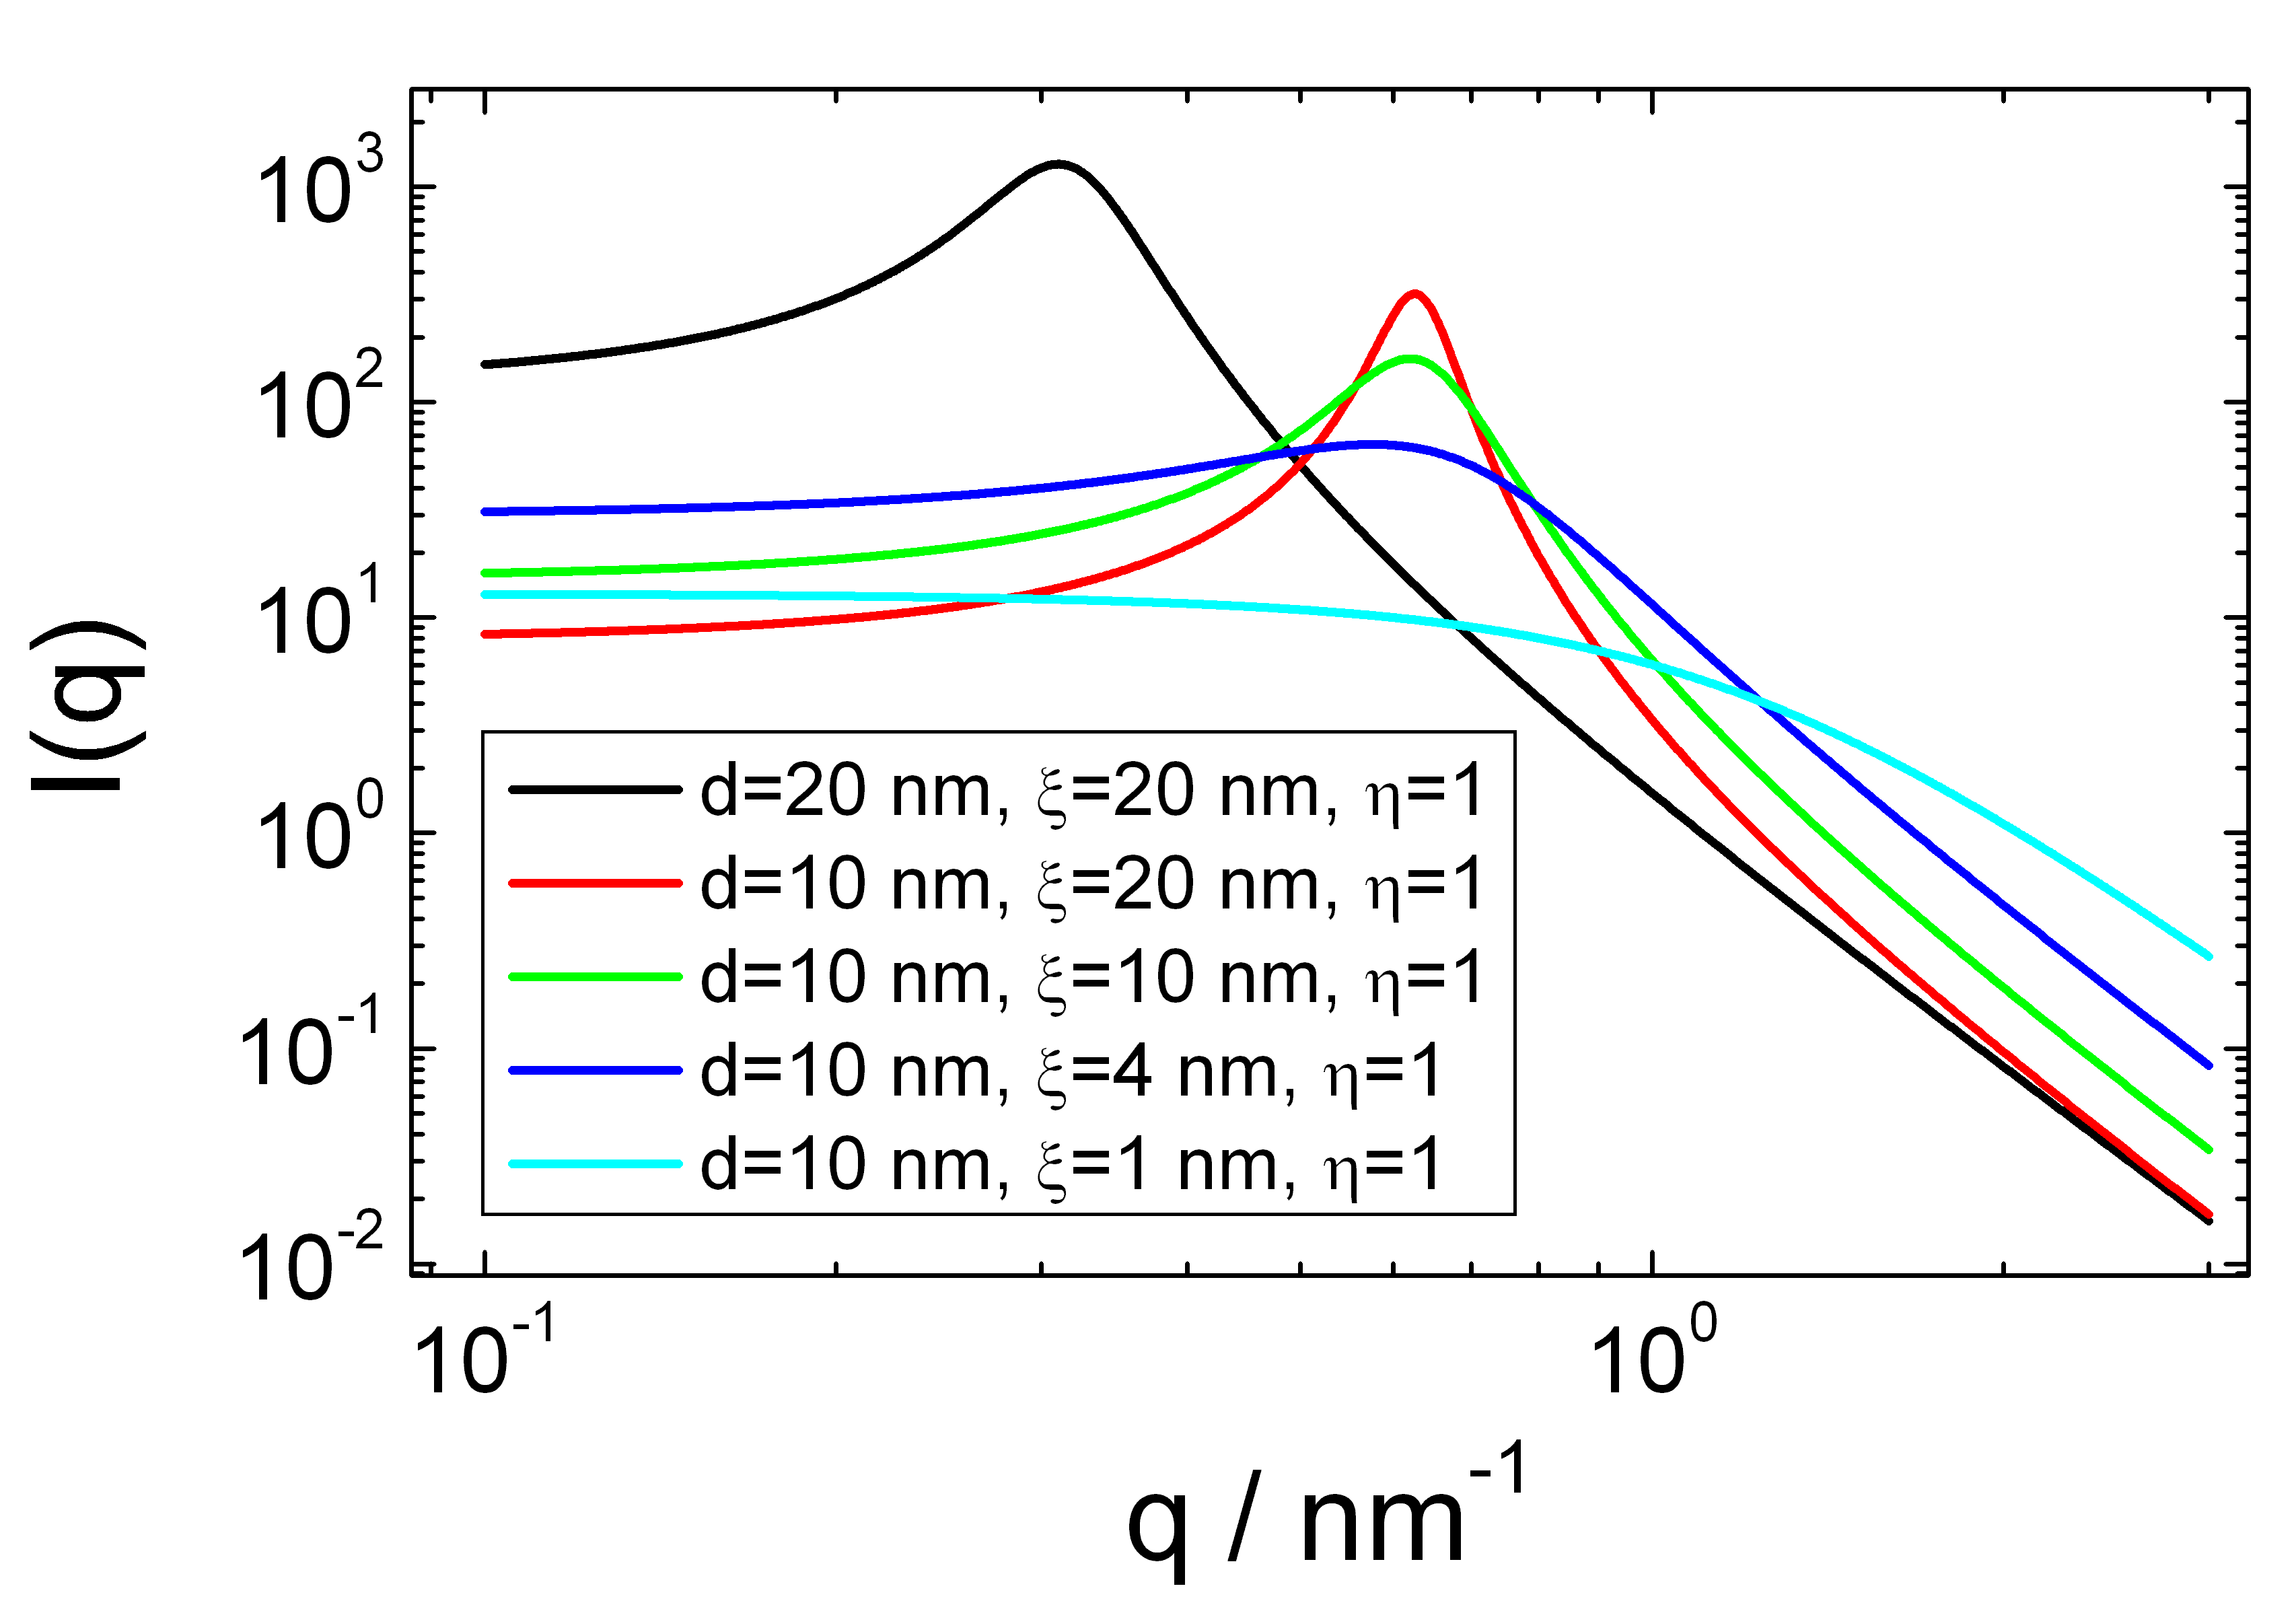
\includegraphics[width=0.85\textwidth]{TeubnerStrey.png}
\end{center}
\caption{Some typical curves for the Teubner-Strey model function} \label{fig:TeubnerStreyIq}
\end{figure}
%\vspace{5mm}
%\noindent REFERENCE:\\
%Teubner, M; Strey, R. J. Chem. Phys., 1987, 87, 3195.\\
%Schubert, K-V.; Strey, R.; Kline, S. R.; and E. W. Kaler J. Chem. Phys., 1994, 101, 5343.

%%%%%%%%%%%%%%%%%%%%%%%%%%%%%%%%%%%%%%%%%%%%%%%%%%%%%%%%%%%%%%%%%%%%%%%%%

\clearpage
\subsection{Debye-Anderson-Brumberger(DAB)}
\label{sect:DAB}~\\

This form factor calculates the scattering from a randomly
distributed (i.e. non-particulate), two-phase system based on the
Debye-Anderson-Brumberger (DAB) \cite{DAB1957,DebyeBueche1949} model
for such systems. The two-phase system is characterized by a single
length scale, the correlation length $\xi$, which is a measure of
the average spacing between regions of phase 1 and phase 2. The
model also assumes smooth interfaces between the phases and hence
exhibits Porod behavior ($I \propto q^{-4}$) at large $q$ ($q \xi
\gg 1$). The pair correlation function is give by
\cite{DebyeBueche1949}
\begin{align}
\gamma(r) = \exp(-r/\xi)
\end{align}
The macroscopic scattering cross-section in the DBA model is given
by
\begin{align}
I(q) = I_0 \frac{1}{\left[1+(q\xi)^2\right]^2}
\end{align}


\underline{Input Parameters for model \texttt{Debye-Anderson-Brumberger}:}\\
\begin{description}
\item[\texttt{xi}] correlation length $\xi$
\item[\texttt{eta}] scattering length density contrast $\Delta\eta$
\end{description}

\underline{Note:}
\begin{itemize}
\item None
\end{itemize}


\begin{figure}[htb]
\begin{center}
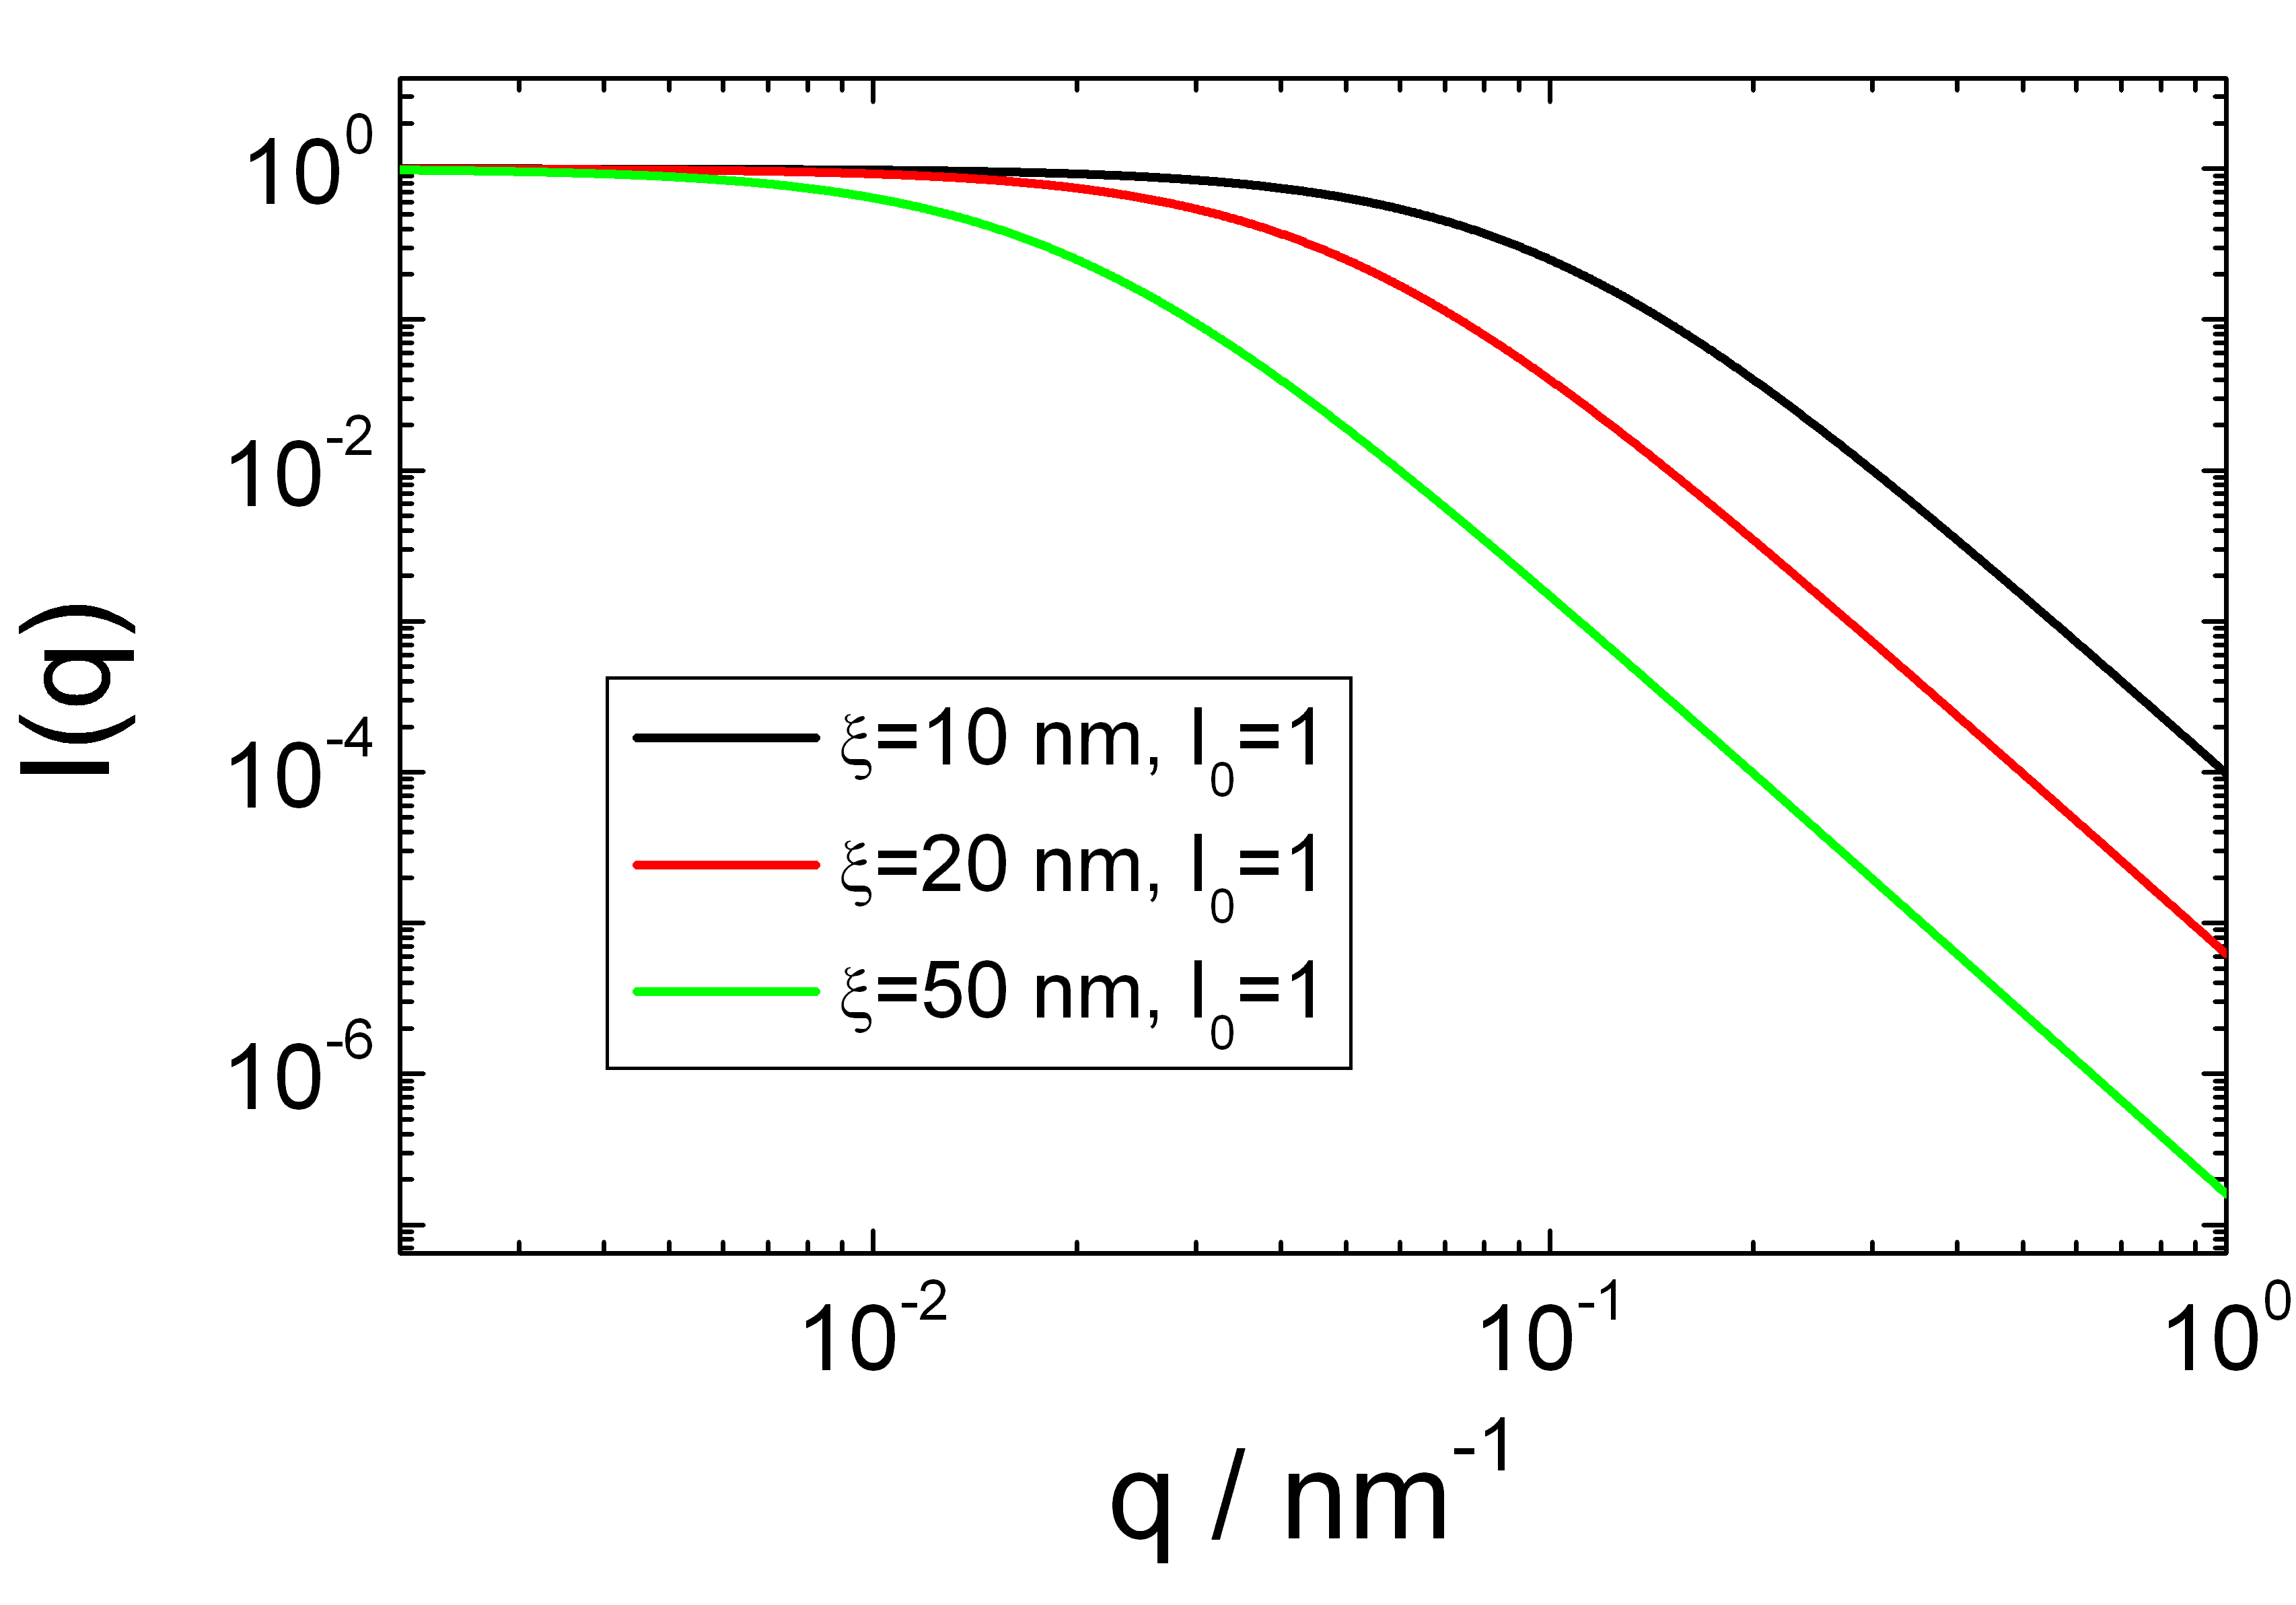
\includegraphics[width=0.85\textwidth]{DAB.png}
\end{center}
\caption{Some typical curves for the Debye-Anderson-Brumberger model function} \label{fig:DABIq}
\end{figure}


%%%%%%%%%%%%%%%%%%%%%%%%%%%%%%%%%%%%%%%%%%%%%%%%%%%%%%%%%%%%%%%%%%%%%%%%%

\clearpage
\subsection{Generalization of the Debye-Anderson-Brumberger model (gDAB)}
\label{sect:gDAB}~\\
The Debye-Anderson-Brumberger(DAB) model from the previous section \ref{sect:DAB} can be considered as a special case from a more general correlation function describing self-affine random density distributions \cite{Klimes2002,Hunter2006,Andersson2008}
\begin{align}
\gamma_0(r) &=
\frac{2}{\Gamma(H)}\left(\frac{r}{2\xi}\right)^H K_H\left(\frac{r}{\xi}\right) \\
\tilde{\gamma}(r) &= \gamma_0(r) \Delta\eta^2 \int_0^\infty \gamma_0(r) 4\pi r^2 \mathrm{d}r = \frac{8\xi^3\pi^{3/2}\Gamma(3/2+H)\Delta\eta^2}{\Gamma(H)}\gamma_0(r)
\end{align}
where $K_n(x)$ is the modified Bessel function of the second kind
and $\Gamma$ is the Gamma function. $H$ is the so-called Hurst
exponent with typical value around $\frac12$. For $H=\frac12$ the gDAB-model results into the DAB model describes in section \ref{sect:DAB}. The scattering intensity is implemented as
\begin{align}
I(q) =  \frac{\pi^3\left(\left(2\xi\right)^3\Gamma(3/2+H)\Delta\eta\right)^2}{\Gamma^2(H)\left[1+(q\xi)^2\right]^{\frac32+H}}
\end{align}


\underline{Input Parameters for model \texttt{gDAB}:}\\
\begin{description}
\item[\texttt{xi}] correlation length $\xi$
\item[\texttt{H}] Hurst exponent $H$
\item[\texttt{eta}] scattering length density contrast $\Delta\eta$
\end{description}

\underline{Note:}
\begin{itemize}
\item None
\end{itemize}


\begin{figure}[htb]
\begin{center}
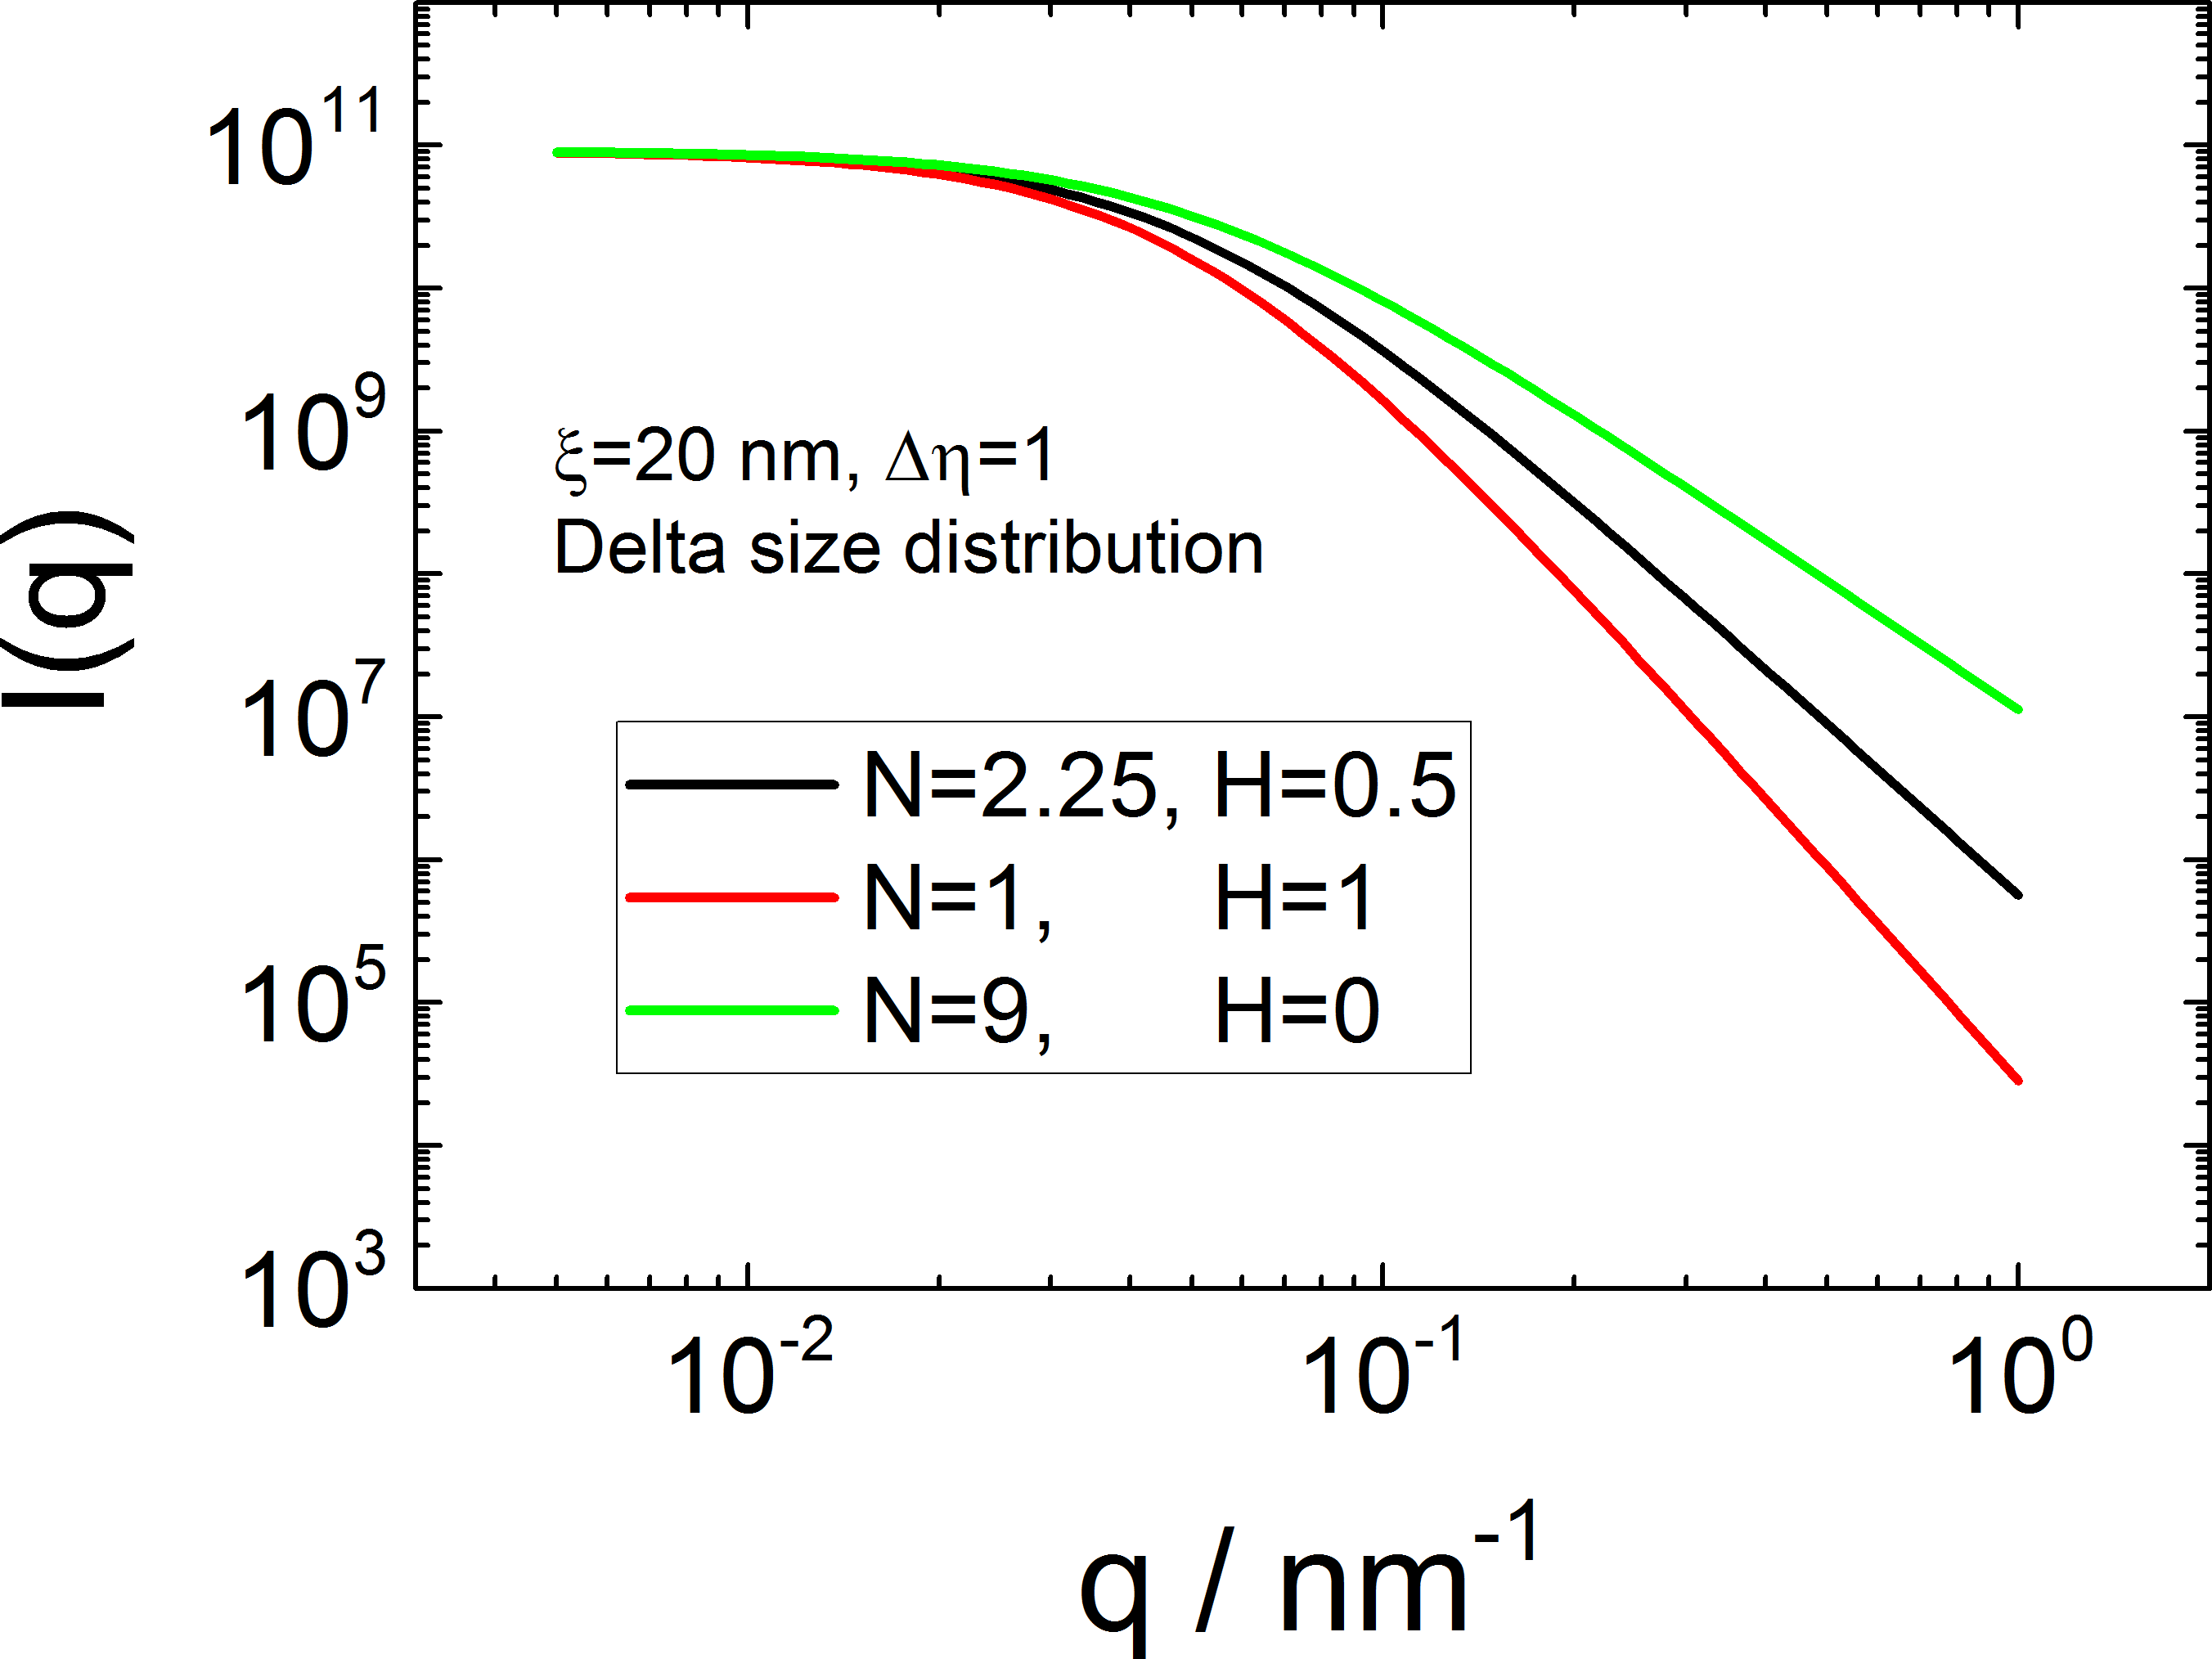
\includegraphics[width=0.85\textwidth]{../images/form_factor/nonparticular/gDAB.png}
\end{center}
\caption{Some typical curves for the generalized Debye-Anderson-Brumberger model function} \label{fig:gDABIq}
\end{figure}

%%%%%%%%%%%%%%%%%%%%%%%%%%%%%%%%%%%%%%%%%%%%%%%%%%%%%%%%%%%%%%%%%%%%%%%%%

\clearpage
\subsection{Spinodal}
\label{sect:Spinodal}
~\\

\begin{figure}[htb]
\begin{center}
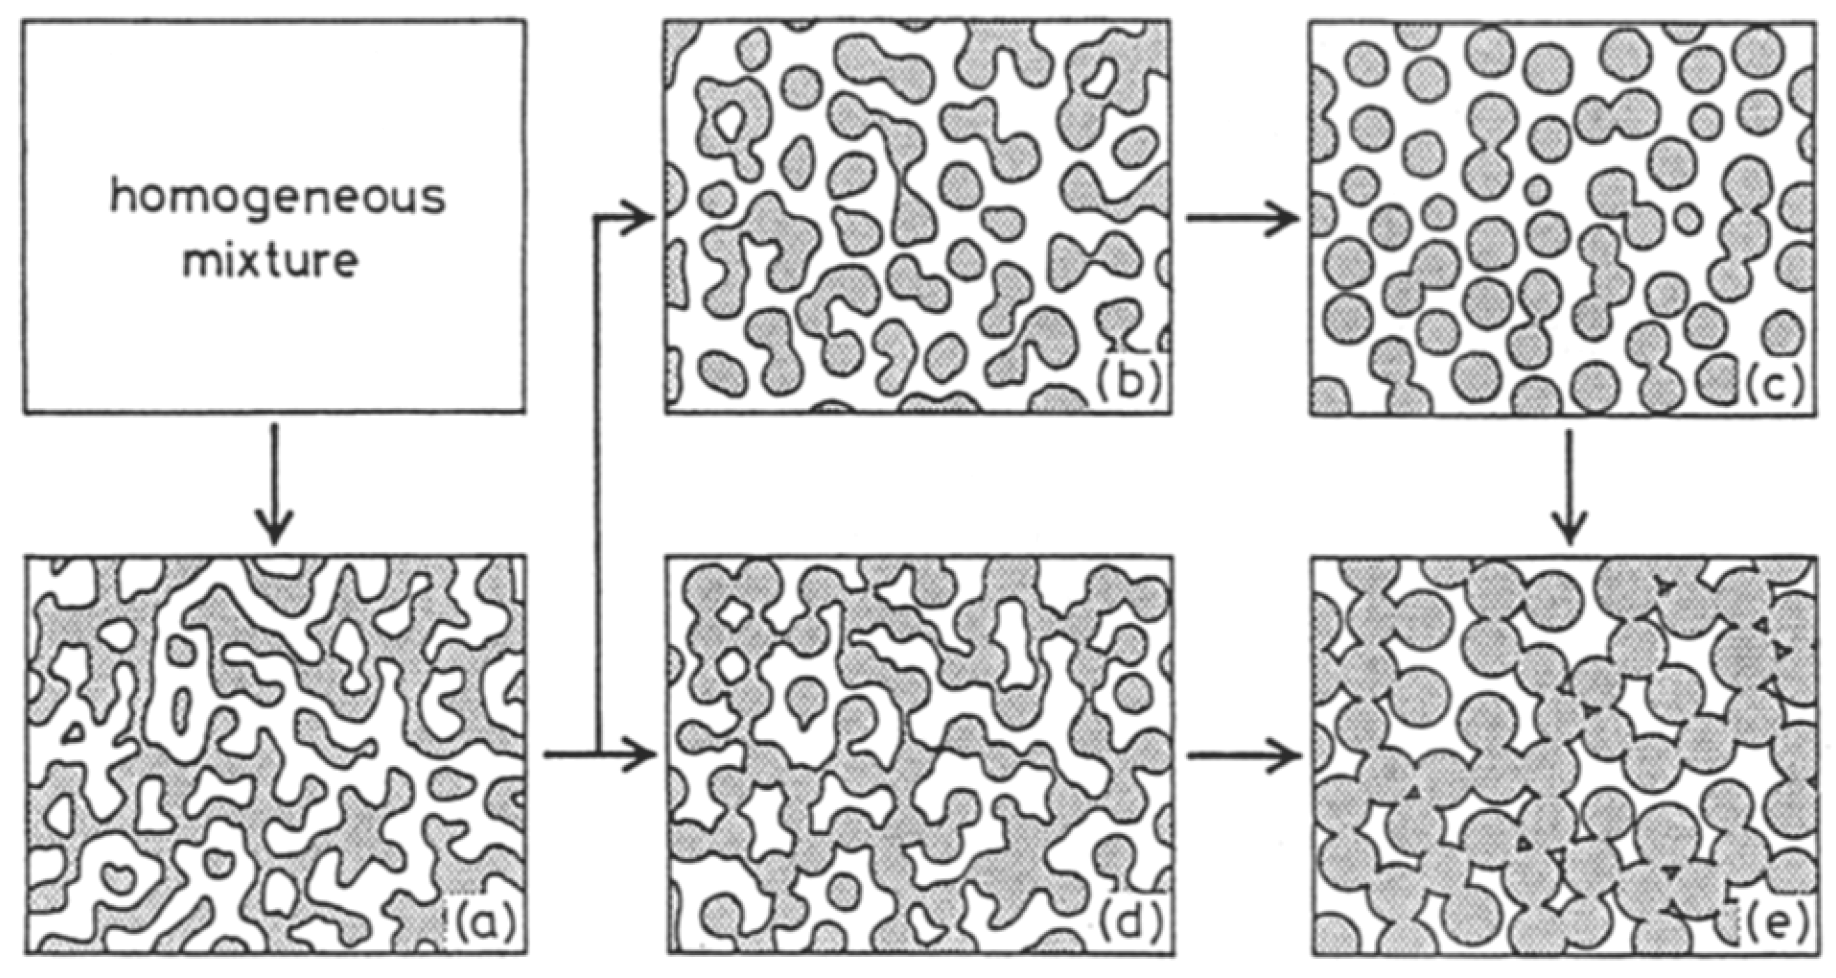
\includegraphics[width=0.648\textwidth]{spinodal2.png}
\end{center}
\caption{Schematic representation of a phase separation scheme
resulting in a connected globule structure.} \label{Spinodal}
\end{figure}

Spinodal decomposing systems show a characteristic small angle
scattering signal with a correlation peak at some scattering value
$q_\text{max}$. The scattering curve $I(q)$ can be approximated by
\begin{align}
I(q) = I_\text{max} \frac{(1+\gamma/2)x^2}{\gamma/2+x^{2+\gamma}}
\end{align}
according to Furukawa \cite{Furukawa1984}, where $x=q/q_\text{max}$.
The position of the correlation peak at $q_\text{max}$ contain
information about the size of the structures, which scatter. The
exponent $\gamma$ is equal to $\gamma=D+1$ for off-critical mixtures
and $\gamma=2D$ for critical concentration mixtures, whereby $D$ is
the dimensionality of the system.

\vspace{5mm}

\underline{Input Parameters for model \texttt{Spinodal}:}\\
\begin{description}
\item[\texttt{Imax}] scattering intensity at peak position $I_\text{max}$
\item[\texttt{Qmax}] peak maximum $q_\text{max}$
\item[\texttt{gamma}] exponent $\gamma$
\end{description}

\underline{Note:}
\begin{itemize}
\item None
\end{itemize}



\begin{figure}[htb]
\begin{center}
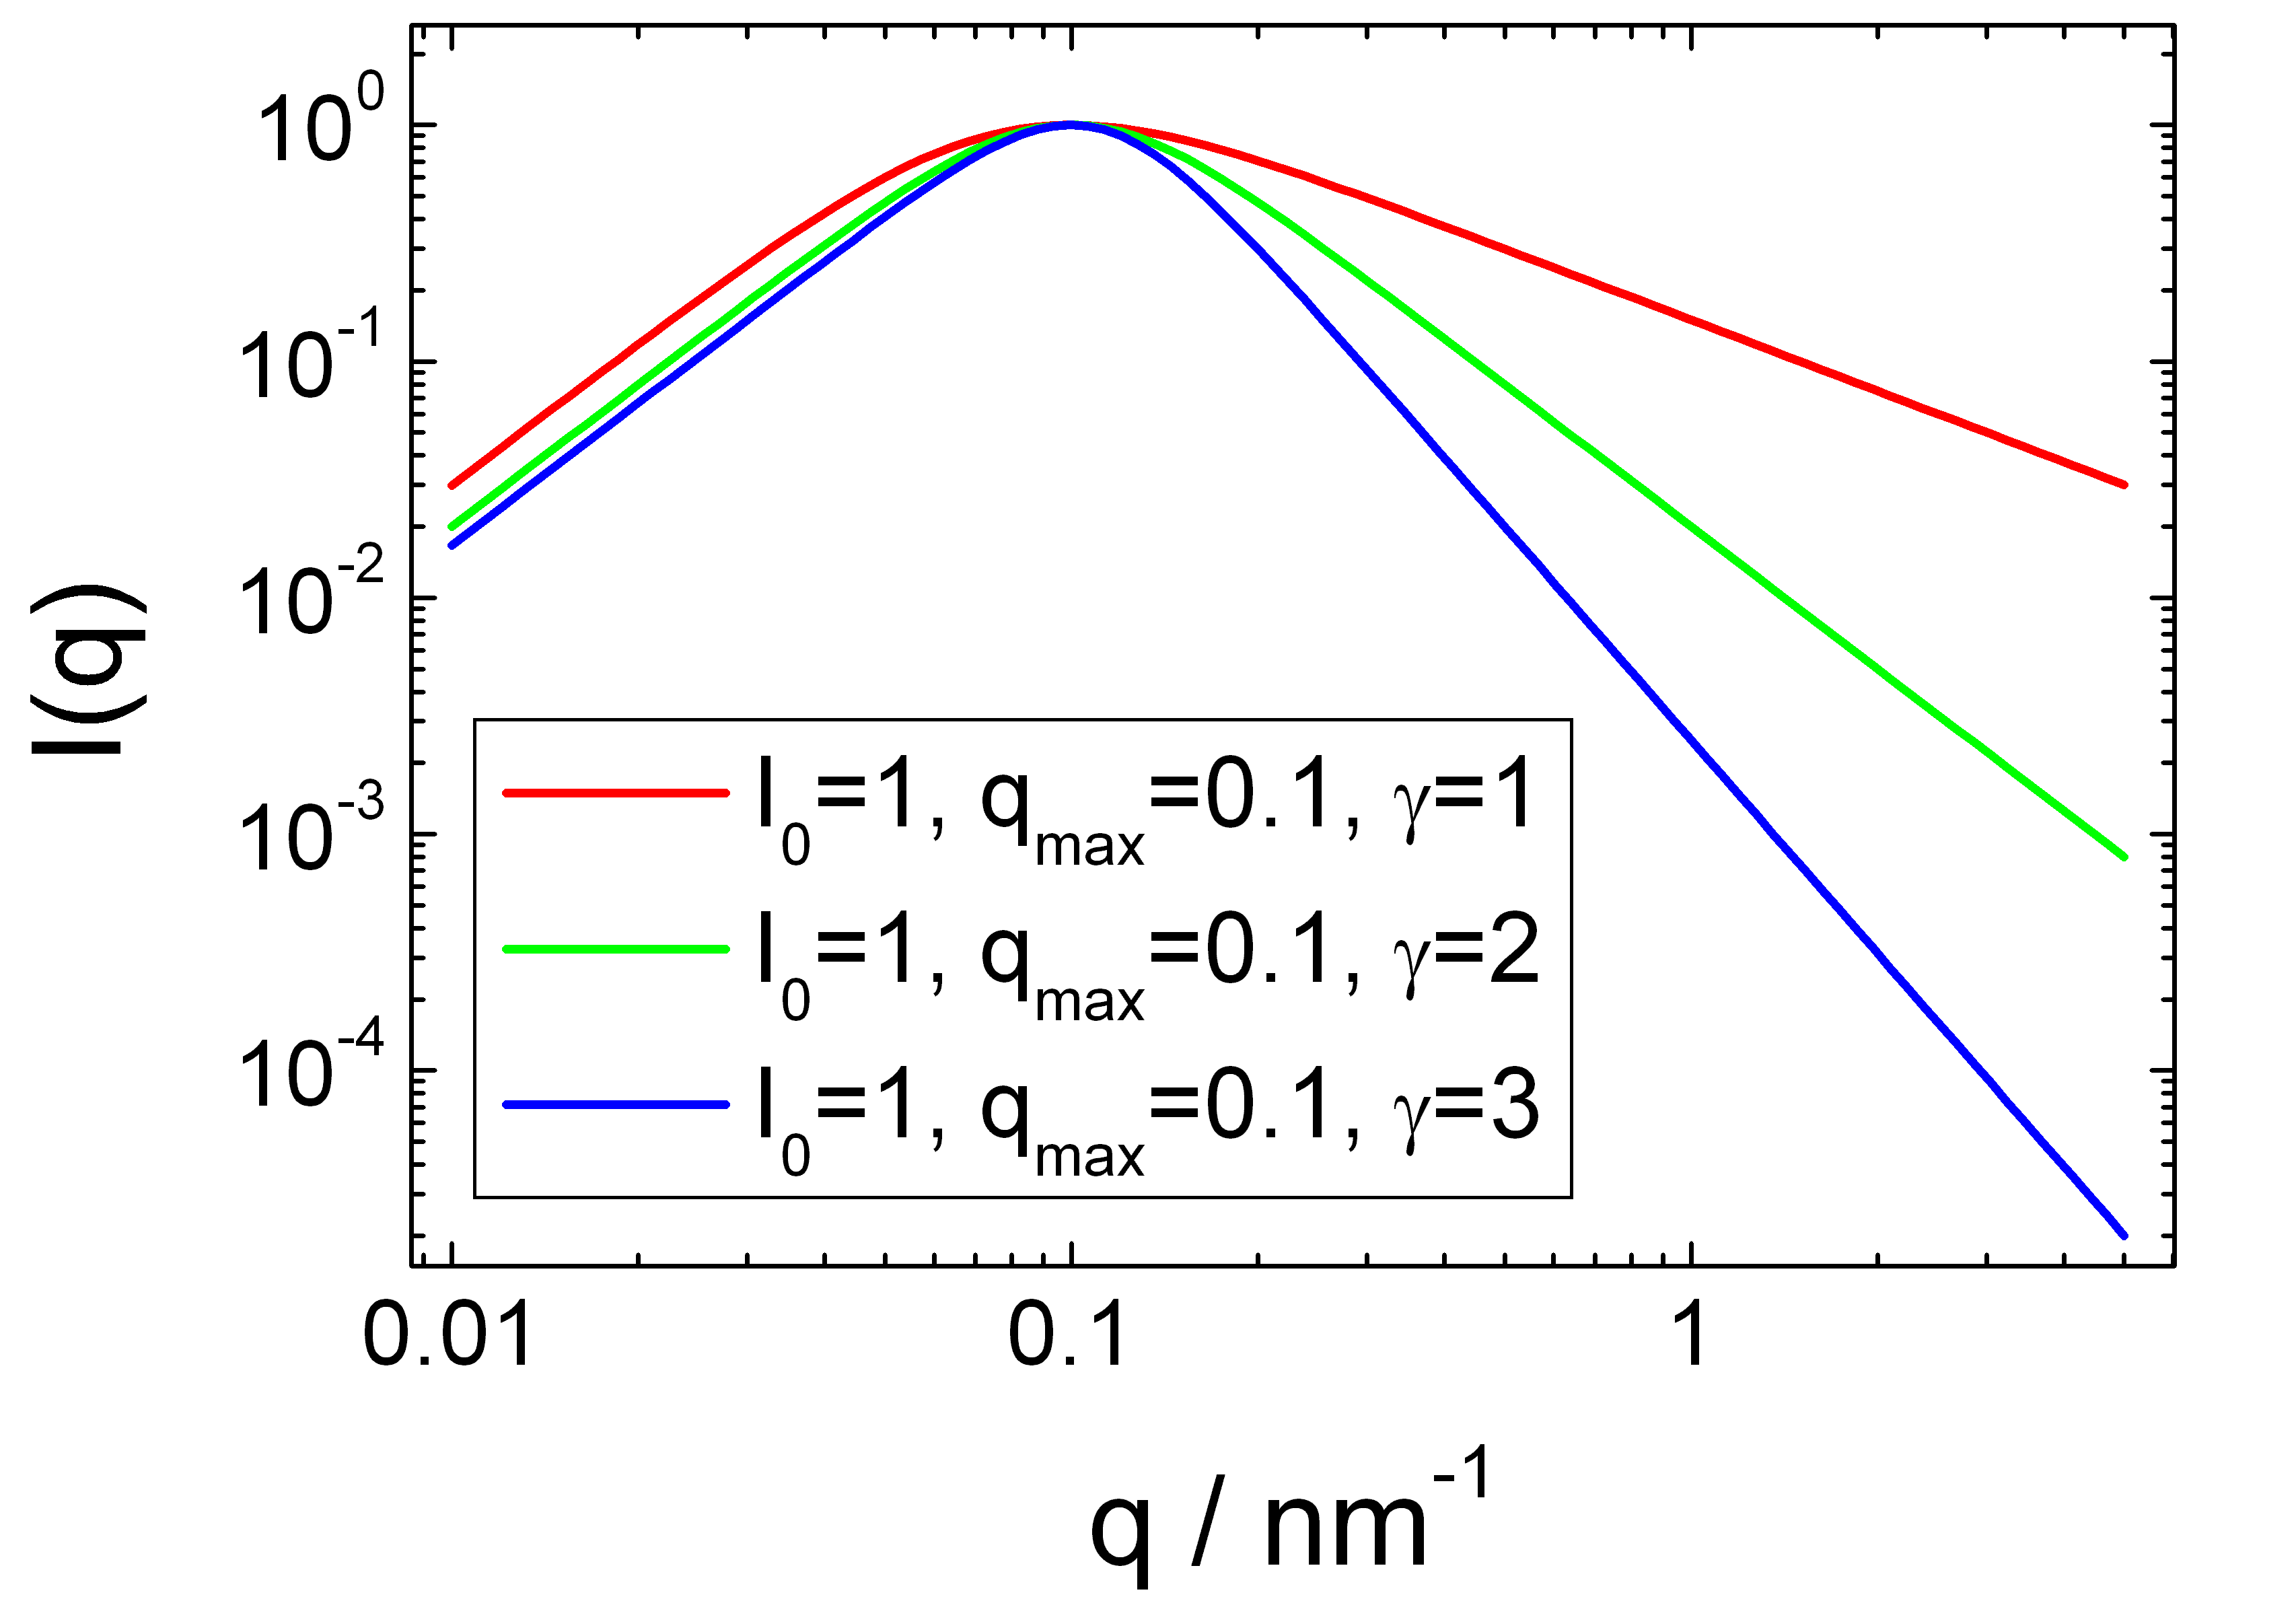
\includegraphics[width=0.85\textwidth]{spinodalIQ.png}
\end{center}
\caption{} \label{fig:spinodalIQ}
\end{figure}

\clearpage
\subsection{OrnsteinZernike}
\label{sect:Zernike}
 ~\\
The low-angle scattering of thermal composition fluctuations can be
described according to the Ornstein-Zernike formulation by a
Lorentzian profile
\begin{align}
I(q) = \frac{I_0}{1+q^2\xi^2}
\end{align}
characterizing the exponential decay of the composition fluctuations
correlation function, with correlation length $\xi$. The Fourier
transform of a Lorentzian function corresponds to correlations dying
out as $\gamma(r) \simeq \frac{1}{r}exp(-r/\xi)$. Note that the
low-$Q$ limit of this emical form reproduces the Guinier law.

\hspace{1pt}\\
\underline{Input Parameters for model \texttt{OrnsteinZernike}:}\\
\begin{description}
\item[\texttt{I0}] forward scattering $I_0$ at $q=0$.
\item[\texttt{xi}] correlation length $\xi$
\end{description}

\begin{figure}[htb]
\begin{center}
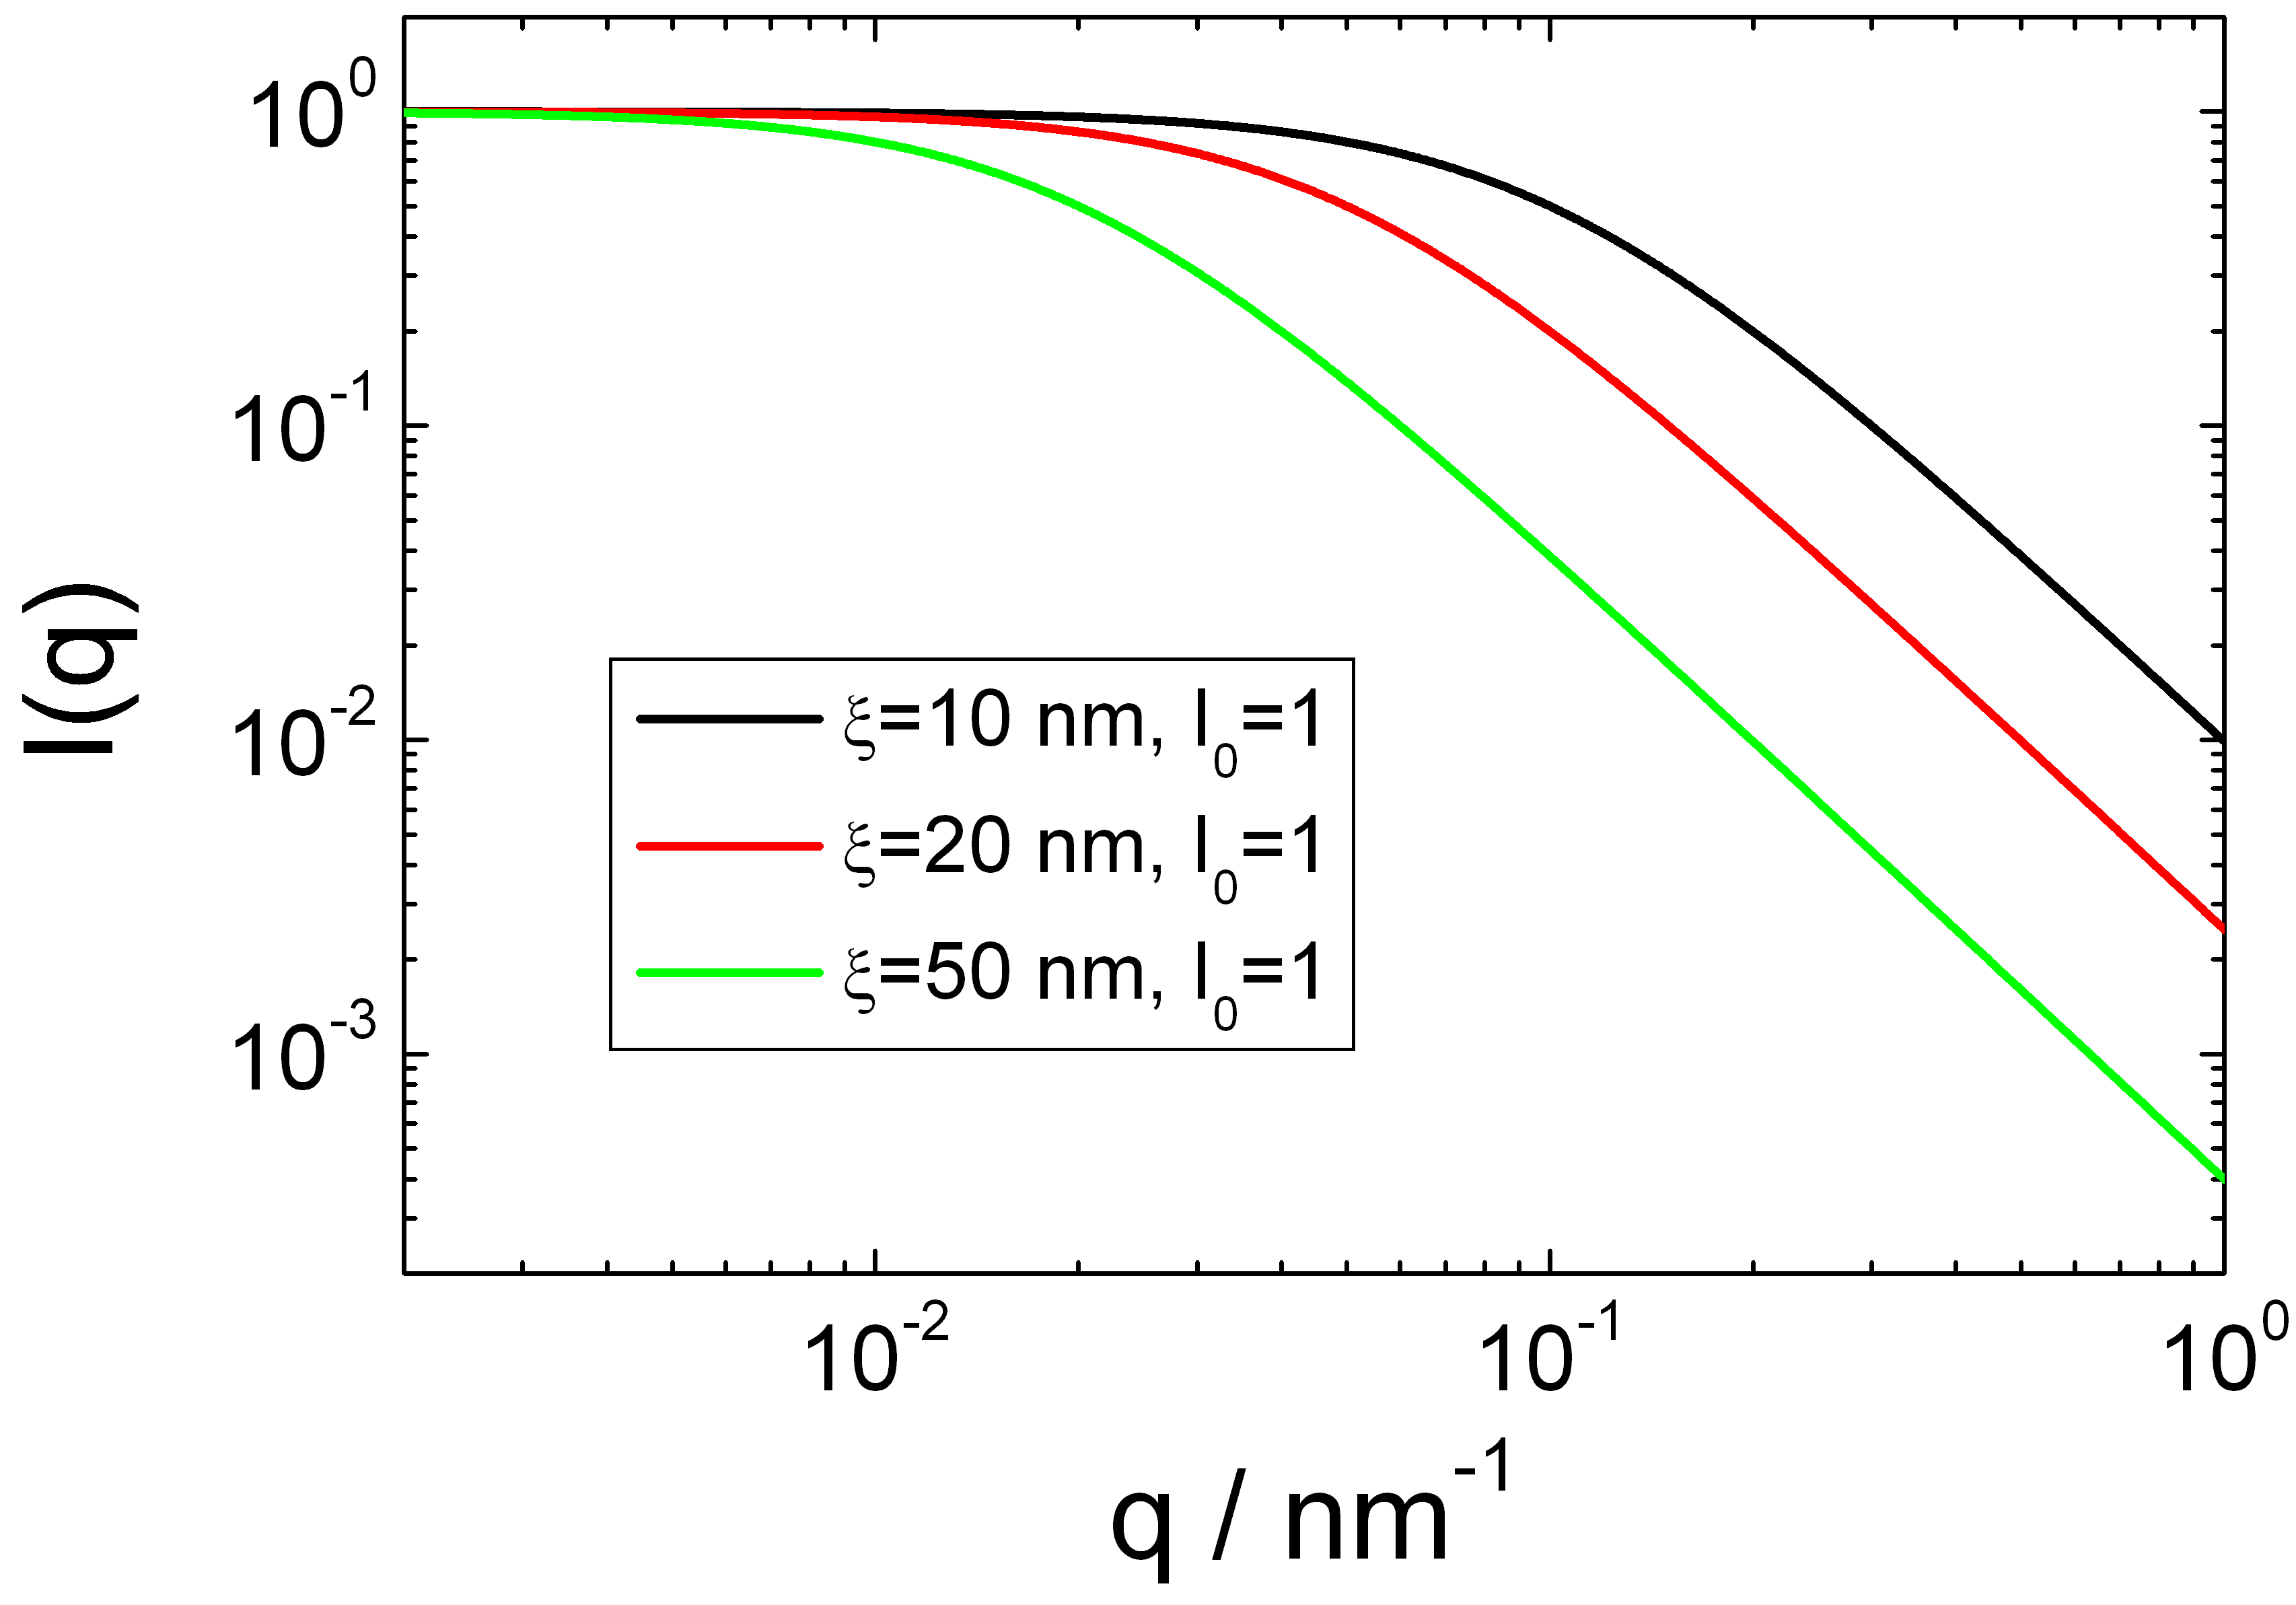
\includegraphics[width=0.85\textwidth]{OrnsteinZernicke.png}
\end{center}
\caption{Ornstein-Zernike Scattering intensity $I(q)$ for different
correlation lengths $\xi$} \label{fig:OrnsteinZernicke}
\end{figure}
\clearpage

\subsection{Broad-Peak}
\label{sect:BroadPeak}
 ~\\
Many SANS spectra are characterized by a broad peak even though they
are from amorphous soft materials. The $d$-spacing corresponding to
the broad peak is a characteristic distance between the scattering
inhomogeneities (such as in lamellar, cylindrical, or spherical
morphologies or for bicontinuous structures). The following simple
functional form reproduces the broad peak feature:
\begin{align}
I(q) = \frac{I_0}{\left(1+\left(\abs{q-q_0}\xi\right)^m\right)^p}
\end{align}
Here the peak position is related to the $d$-spacing as $q_0 =
2\pi/d$. Soft systems that show a SANS peak include copolymers,
polyelectrolytes, multiphase systems, layered structures, etc.

\hspace{1pt}\\
\underline{Input Parameters for model \texttt{Broad-Peak}:}\\
\begin{description}
\item[\texttt{I0}] scattering intensity $I(q)$ at $q=q_0$.
\item[\texttt{xi}] correlation length $\xi$
\item[\texttt{m}] exponent $m$
\item[\texttt{p}] exponent $p$
\end{description}

\hspace{1pt}\\
\underline{Note:}
\begin{itemize}
\item For $q_0=0$, $m=2$ and $p=1$ one gets the Ornstein-Zernike model.
\item For $q_0=0$, $m=2$ and $p=2$ The Broad-Peak model is identical to the Debye-Anderson-Brumberger model.
\end{itemize}

\begin{figure}[htb]
\begin{center}
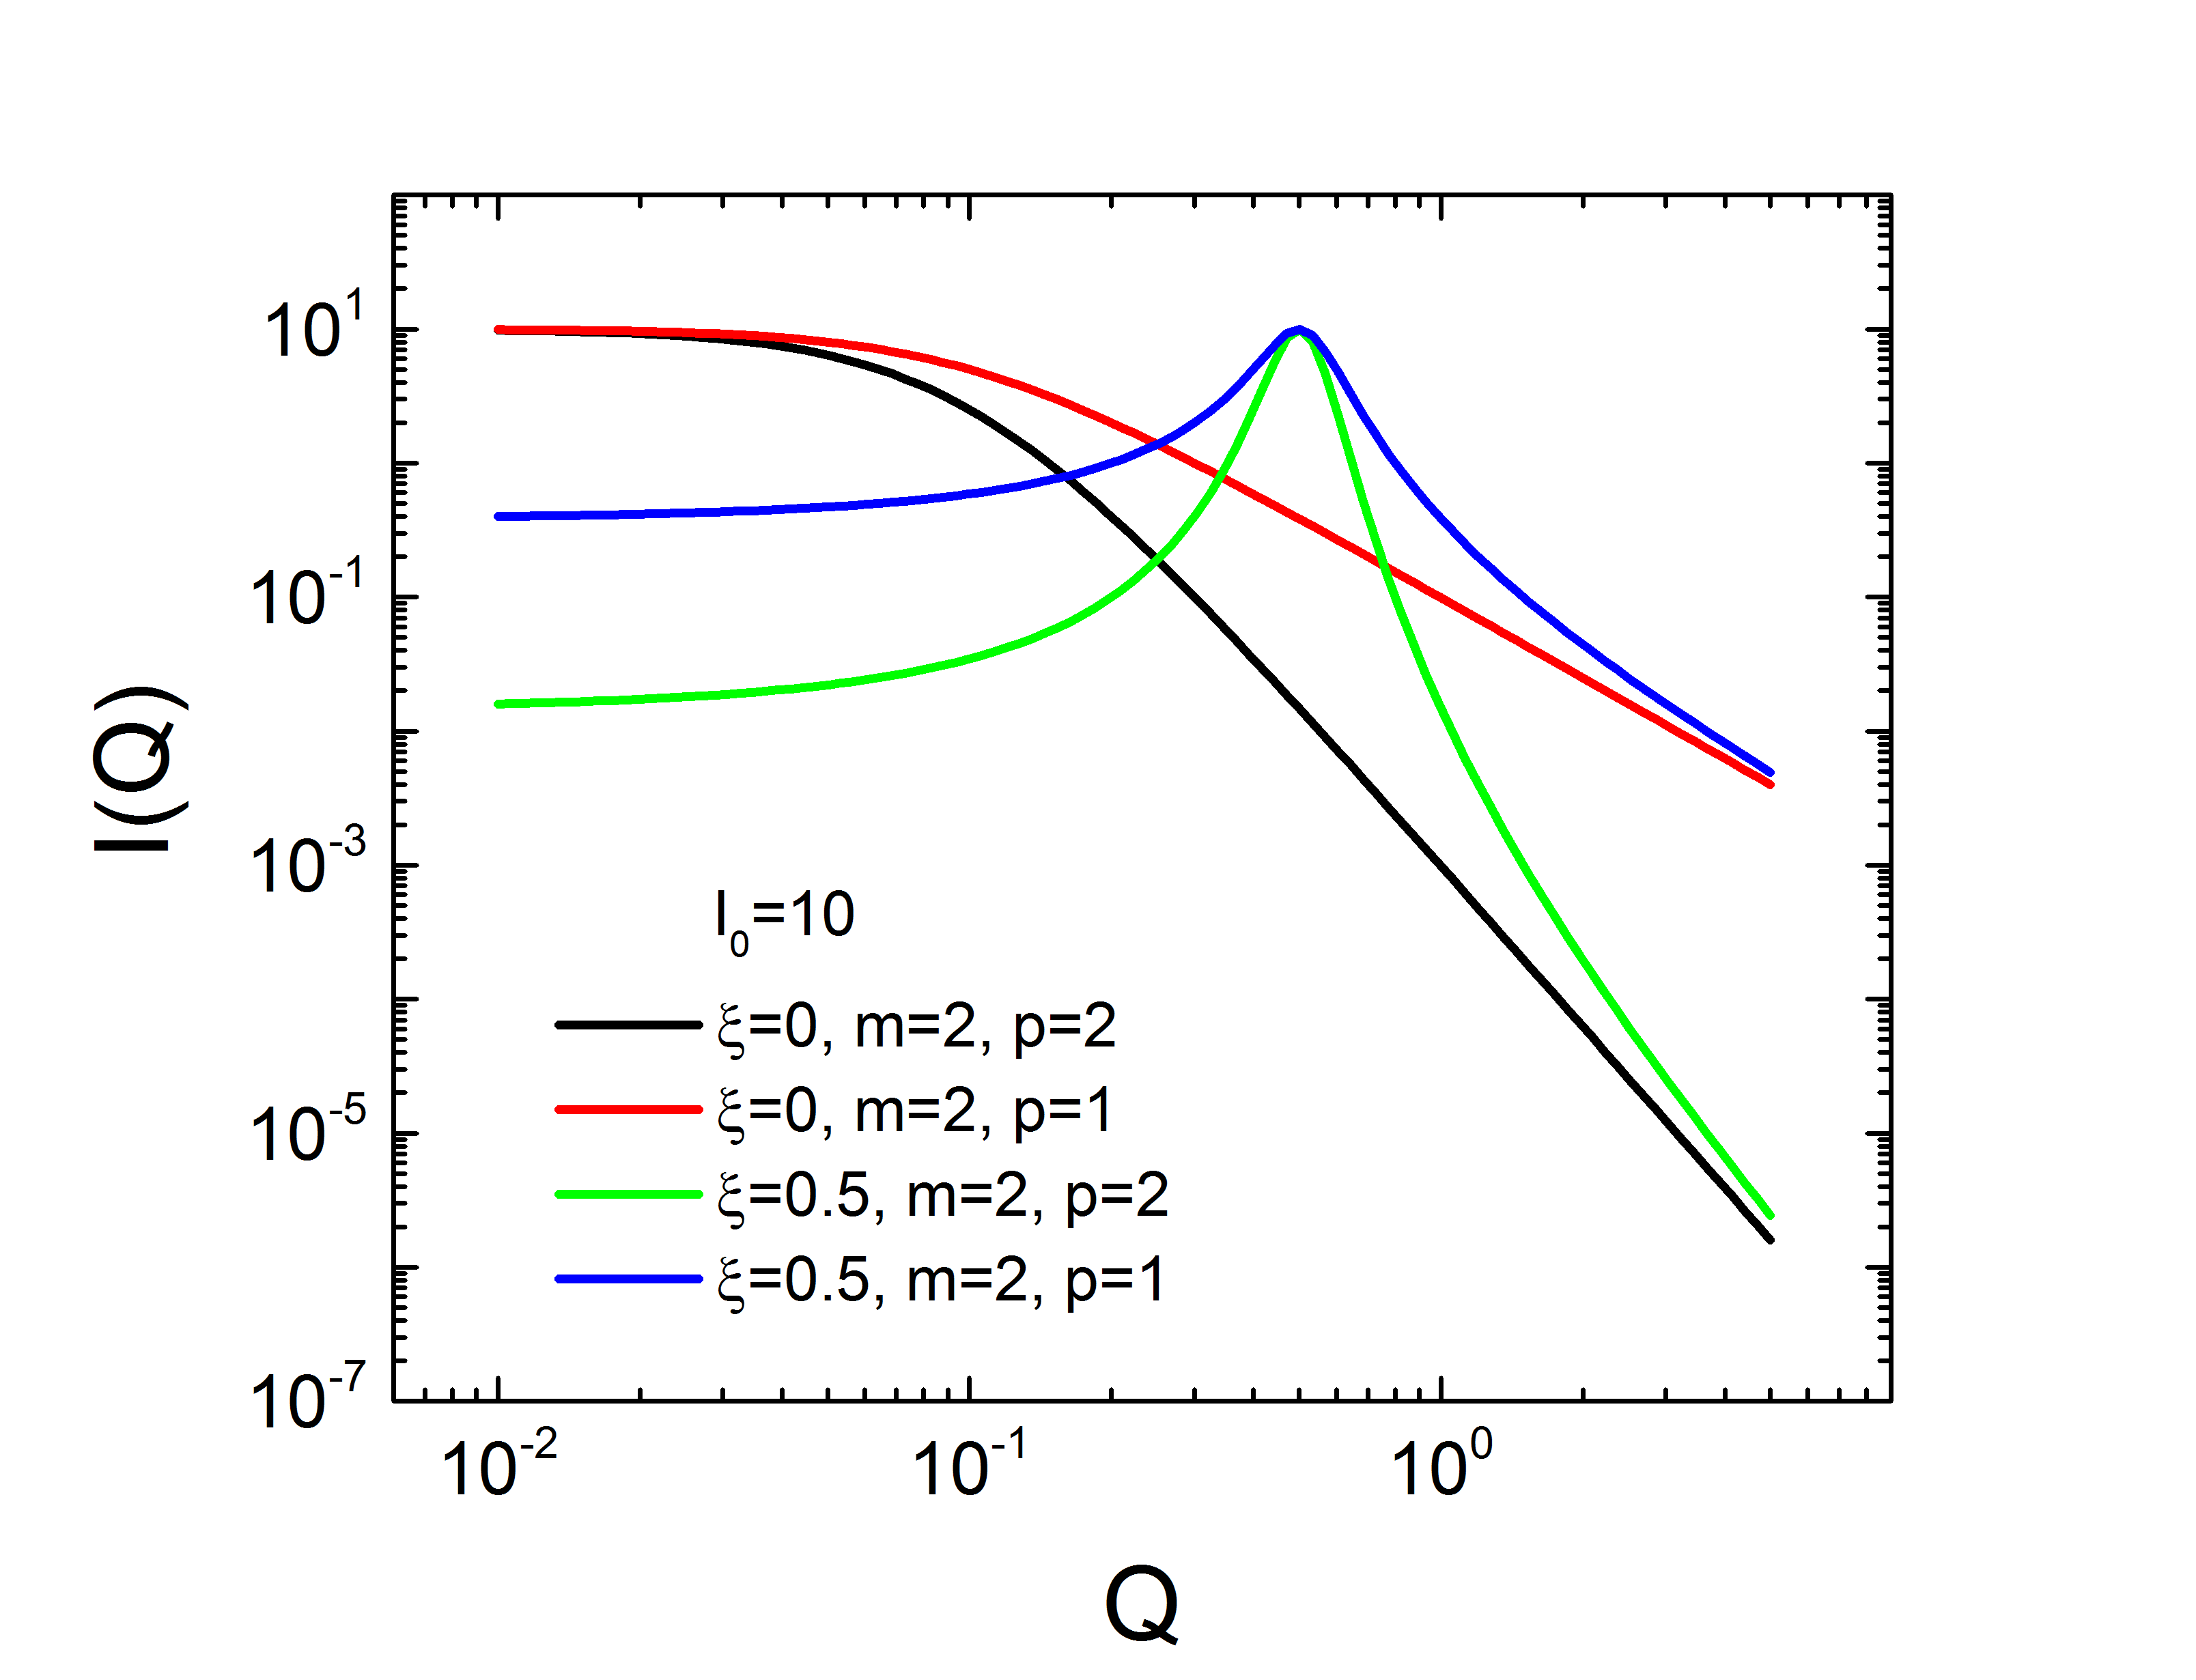
\includegraphics[width=0.85\textwidth]{BroadPeak.png}
\end{center}
\caption{Empirical form factor of Broad-Peak} \label{fig:BroadPeakIq}
\end{figure}

\clearpage
\subsection{generalized Guinier approximation \cite{Fratzl1994,Hjelm1992,Hjelm1995,Hjelm2000}}
\label{sec:generalizedGuinier}  ~\\

\begin{figure}[htb]
\begin{center}
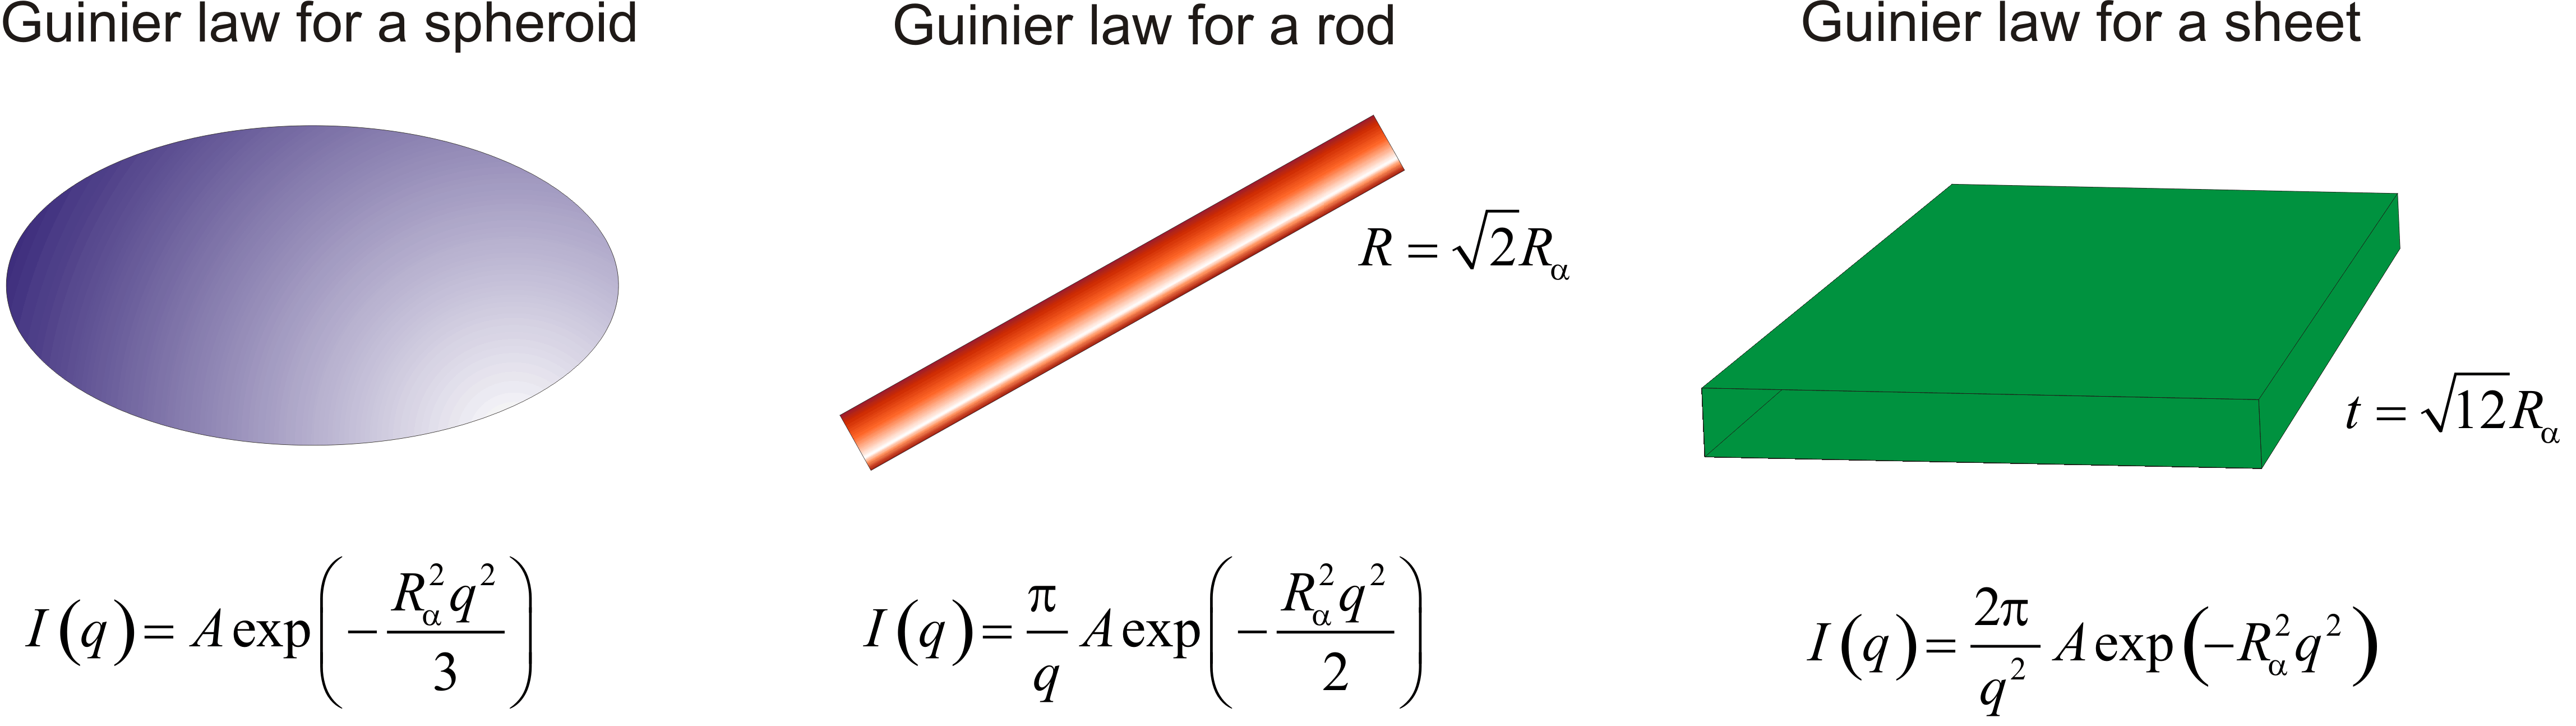
\includegraphics[width=0.75\textwidth]{generalizedGuinier_q.png}
\end{center}
\caption{generalized Guinier approximation}
\end{figure}
Quantitative analysis of particle size and shape starts with the
Guinier approximations. For three-dimensional objects the Guinier
approximation is given by $I(q) = \exp(-Rg^2q^2/3)$ This
approximation can be extended also to rod-like and plane objects by
\begin{align}
I(q) &= \left\{
\begin{array}{lll}
  1 & \mbox{for} & \alpha=0 \\
  \alpha \pi q^{-\alpha} & \mbox{for} & \alpha=1,2 \\
\end{array}
\right\} A \,\, \exp\left(-\frac{R_\alpha^2 q^2}{3-\alpha}\right)
\label{eq:generalizedGuinier}
\end{align}
\begin{description}
\item[$\alpha=0$] spheroid
\item[$\alpha=1$] rod-like
\item[$\alpha=2$] plane
\end{description}
The apparent particle shape (also called the dimensionality) is
represented in eq.\ \ref{eq:generalizedGuinier} by $\alpha$, which
has integer values of 0, 1, and 2 for a point, a line, and a plane,
respectively. Equation \ref{eq:generalizedGuinier} states that there
are $q$ ranges, corresponding to length scales as $q^{-1}$, from
which the particle dimension or shape, $\alpha$, the radius of
gyration, $R_\alpha$, and the pre-factor, $A$, characteristic of
$\alpha$ can be inferred. $\alpha$ has a value of 0 for a $q$ range
such that $qR_g < 1-1.3$ (the larger applies when the particle is
known to be a spheroid), where $R_g$ is the particle radius of
gyration (computed about the particle centroid). In this case, the
pre-factor $A$ describes the excess differential cross-section per
unit mass (cm$^2$ g$^{-1}$) of a particle. If the particle has one
dimension of length $L$, that is, much larger than the others (i.e.,
elongated, rod-like, or worm-like), then there is a $q$ range such
that $qR_c < 1 \ll qL$, where $\alpha = 1$. Here, $R_c$ is the
radius of gyration (computed about a line centered along $L$) of the
cross-section perpendicular to $L$. If these conditions apply, the
pre-factor $A$ describes the excess differential cross section per
unit length per unit mass (cm$^2$ \AA$^{-1}$ g$^{-1}$). Finally, for
planar shapes, including single bilayer vesicles, with two locally
large dimensions, $D$, and planar cross-sectional radius of gyration
(computed about a central plain),$R_d$, there may be a region of $q$
such that $qR_d < 1 \ll qD$, where $\alpha = 2$. For such planar
structures, the pre-factor is the excess differential cross-section
per unit area per unit mass (cm$^2$ \AA$^{-2}$ g$^{-1}$) of a sheet.

\newpage
\hspace{1pt}\\
\underline{Input Parameters for model \texttt{generalized Guinier law}:}\\
\begin{description}
\item[\texttt{I0}] scaling factor $I0$.
\item[\texttt{a}]  dimensionality parameter $\alpha$ for potential law at small
     $Q$-values; $\alpha=0$: sphere, $\alpha=1$: rod, $\alpha=2$: lamellar
\item[\texttt{Ra}] radius of gyration $R_{a}$
\end{description}

\hspace{1pt}\\
\underline{Note:}
\begin{itemize}
\item parameter constrain: $3>\alpha\geq 0$
\end{itemize}

\begin{figure}[htb]
\begin{center}
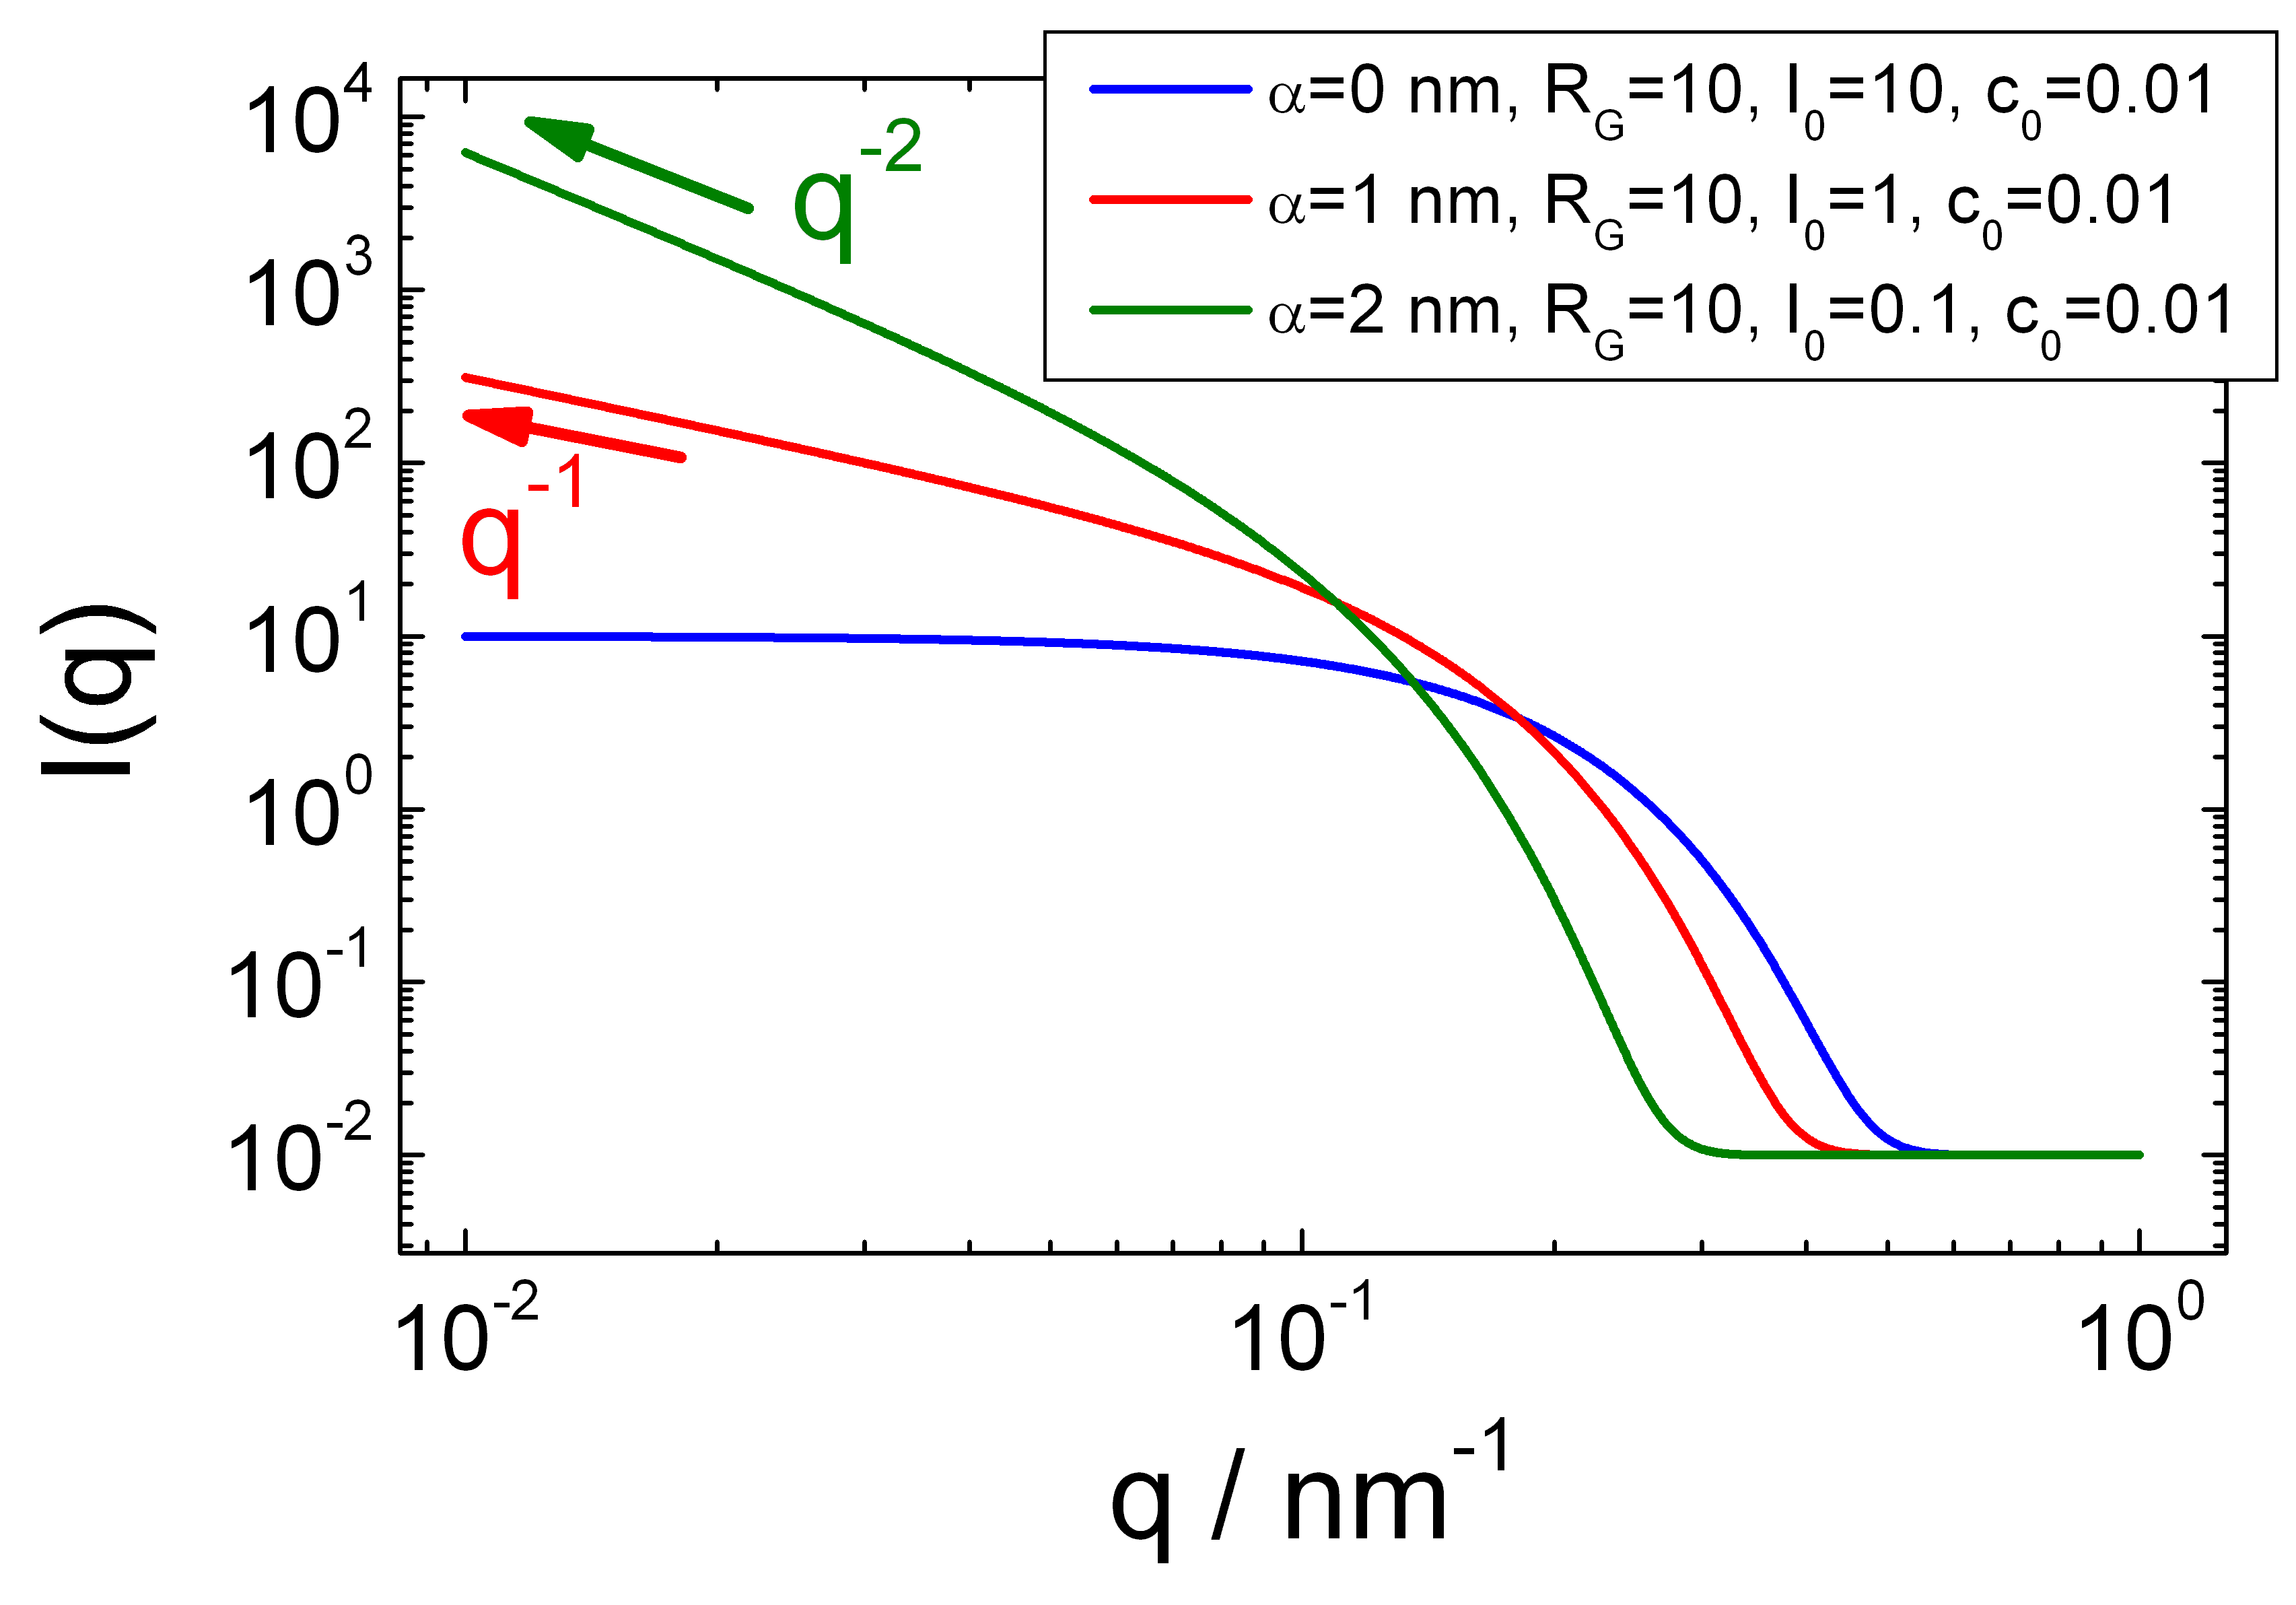
\includegraphics[width=0.85\textwidth]{generalizedGuinierIq.png}
\end{center}
\caption{generalized Guinier law} \label{fig:generalizedGuinierIq}
\end{figure}

\clearpage
\subsection{generalized Guinier-Porod law}
\label{sec:generalizedGuinierPorodLaw}  ~\\

The generalised Guinier-Porod approach from \cite{Hammouda2010} combined the  generalized Guinier approximation \ref{sec:generalizedGuinier} with a potential law.

\begin{align}
I(q) &=
\begin{cases}
  \frac{G_2}{Q^{s_2}} \exp\left(-\frac{Q^2R^2_{g2}}{3-s_2}\right)& \mbox{for } Q \leq Q_2\\
  \frac{G_1}{Q^{s_1}} \exp\left(-\frac{Q^2R^2_{g1}}{3-s_1}\right)& \mbox{for } Q_2 < Q\leq Q_1\\
  \frac{D}{Q^m} & \mbox{for } Q > Q_1 \\
\end{cases}
\label{eq:generalizedGuinierPorod}
\end{align}
To get a continuous function in $I(Q)$ and its derivative yield constrains for two parameters, which have been chosen to be $Q_2$ and $G_2$, for which one get
\begin{align}
Q_2 &= \sqrt{\frac{s_1-s_2}{\frac{2}{3-s_2}R^2_{g2}-\frac{2}{3-s_1}R^2_{g1}}}\\
G_1 &= G_2 \exp\left[-Q_2^2\left(\frac{R^2_{g1}}{3-s_1}-\frac{R_{g2}^2}{3-s_2}\right)\right] Q_2^{(s_2-s_1)} \\
Q_1 &= \frac{1}{R_{g1}}\sqrt{\left(m-s_1\right)\frac{3-s_1}{2}} \\
D   &= G_1 \exp\left(-\frac{Q_1^2 R_{g1}^2}{3-s_1}\right) Q_1^{m-s_1}
\label{eq:generalizedGuinierPorodConstrains}
\end{align}
The constrains for the parameters are $R_{g2}>R_{g1}$, $3>s_1>s_2$, and $m>s_1$. The reason for that is, that the functions and their derivatives used in \ref{eq:generalizedGuinierPorod} are strongly monotonic decaying and the constrains are required to get a continuous function and derivative at $Q_1$ and $Q_2$.

\hspace{1pt}\\
\underline{Input Parameters for model \texttt{generalized Guinier-Porod law}:}\\
\begin{description}
\item[\texttt{G2}] scaling factor $G_2$.
\item[\texttt{s2}] potential law for the small $Q$-region, $s_2$ is a dimensionality parameter
\item[\texttt{RG2}] radius of gyration $R_{g2}$ (larger dimension)
\item[\texttt{s1}] potential law in intermediate $Q$-range, $s_1$ is a dimensionality parameter
\item[\texttt{RG1}] radius of gyration $R_{g1}$ (smaller dimension)
\item[\texttt{m}] potential law at large $Q$-value: $Q^{-m}$
\end{description}

\hspace{1pt}\\
\underline{Note:}
\begin{itemize}
\item parameter constrain: $R_{g2}>R_{g1}$
\item parameter constrain: $3>s_1>s_2$
\item parameter constrain: $m>s_1$
\end{itemize}

\begin{figure}[htb]
\begin{center}
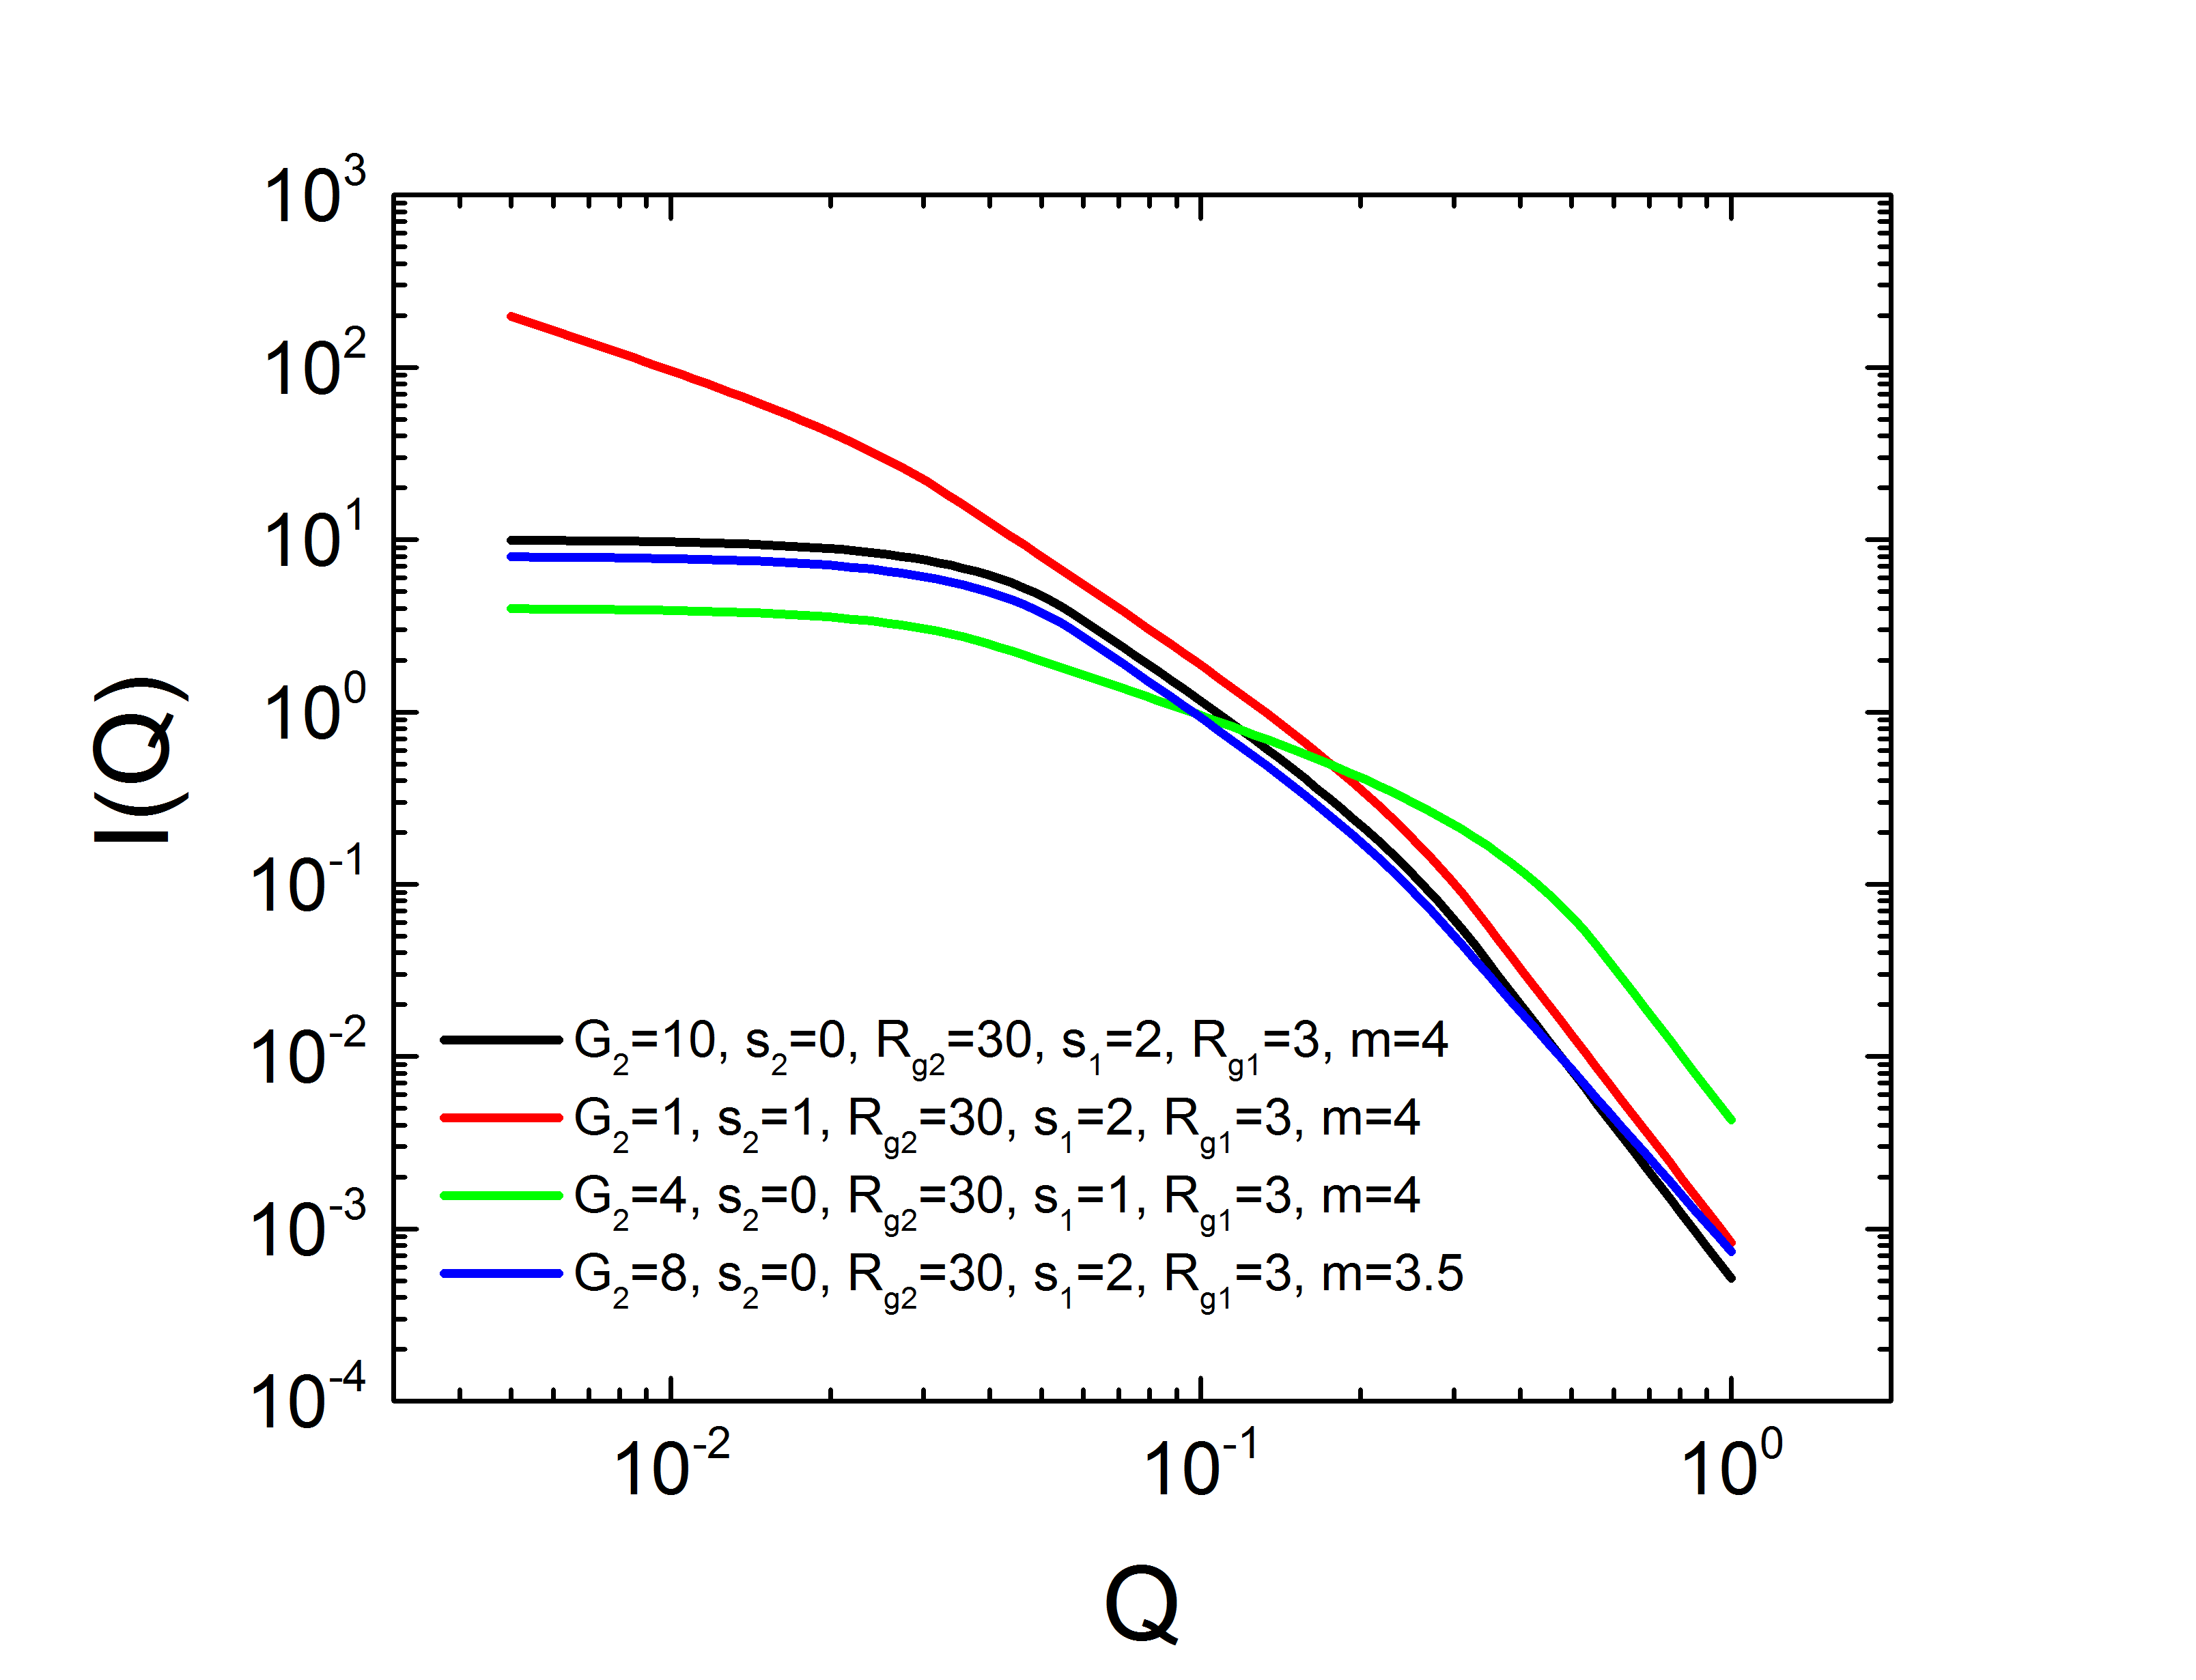
\includegraphics[width=0.85\textwidth]{GuinierPorodIQ.png}
\end{center}
\caption{some examples showing the behaviour of the generalized Guinier-Porod law} \label{fig:GuinierPorodIQ}
\end{figure} 